% \newcommand*{\NoMarkdown}{}

%TODO: once the text is "finished": [see sublime note]
% see also: https://www.wiwi.uni-osnabrueck.de/fileadmin/documents/public/3_fachgebiete/3.11_mikro/Guidelines/Guidelines_Thesis.pdf

% NoMarkdown and Twoside are compile-commands, see https://tex.stackexchange.com/a/220101/108199, https://tex.stackexchange.com/a/22525/108199, https://tex.stackexchange.com/a/33577/108199

\ifdefined\ForPrinting
	\PassOptionsToClass{twoside}{scrreprt}
	\PassOptionsToPackage{colorlinks=false}{hyperref}
\else
	\PassOptionsToPackage{colorlinks=true}{hyperref}
\fi

\documentclass[11pt,
  paper=a4, 
%   twoside,
%   openright,
  hidelinks,
  bibliography=totocnumbered,
	captions=tableheading,
	BCOR=10mm
]{scrreprt}

% ====================== /parts from MastersDoctoralThesis.cls ======================
%	HEADERS AND FOOTERS

\usepackage[automark,headsepline]{scrlayer-scrpage} %https://esc-now.de/_/latex-individuelle-kopf--und-fusszeilen-update/?lang=de
\pagestyle{scrheadings}
\clearpairofpagestyles
% \automark*[section]{chapter} %[] = right side, {} = left side
\ifdefined\ForPrinting
	\automark*[section]{chapter}
\else
	\automark*[chapter]{section}
\fi
% TODO: maybe have a SEPARATE automark for ONE-sided, wo's section ist?!
\ihead{\headmark}% Inner header
\ohead[\pagemark]{\pagemark}% Outer header
\ifoot{}% Inner footer
\ofoot{}% Outer footer
%TODO: check vor dem Drucken, ich bin gerade etwas verwirrt was wo wann. 
% Ich dachte bei Okular: View Mode -> "Facing Pages, first centered" ist wie ich es gedruckt auch hab, aber scheinbar krieg ich genau die non-facing pages da als facing angezeigt? Und for some reason geht nur \automark[section]{chapter} und nicht \automark[chapter]{section}, was falsch rum aussieht? wie dumm?! Wenn ich das mit Okular wie gesagt anzeige sind halt auch inner und outer head vertauscht... Maybe I need the doc-class-option "openright"?? 
%TODO: create final PDF at least twice, once with twoside and once without
%TODO: on the two-sided version, addtitionally have \automark*[section]{chapter}

% ====================== /parts from MastersDoctoralThesis.cls ======================

\newcommand{\saveref}[2]{\texorpdfstring{\hyperref[#1]{#2}}{#2}}


% ====
% https://tex.stackexchange.com/a/135731/108199
\newcounter{saveenumerate}
\makeatletter
\newcommand{\enumeratext}[1]{%
	\setcounter{saveenumerate}{\value{enum\romannumeral\the\@enumdepth}}
	\end{enumerate}
	#1
	\begin{enumerate}
	\setcounter{enum\romannumeral\the\@enumdepth}{\value{saveenumerate}}%
}
\makeatother

\usepackage{changepage} %https://tex.stackexchange.com/a/594/108199
\newcommand{\itemtextCore}[1]{%
	\begin{adjustwidth}{0.2\textwidth}{0cm}
	\begin{flushright}
	{   
		\parskip=0pt
		\small
		\vspace{-0.55em}
		\textit{#1}
		\vspace{-0.55em}
	}
	\end{flushright}
	\end{adjustwidth}
}

\newcommand{\itemtext}[1]{%
	\end{itemize} 
	\itemtextCore{#1}
	\begin{itemize}
}
% for the last one I have to use this, because otherwise I'll get a "missing \item" error
\newcommand{\lastitemtext}[1]{%
	\end{itemize} 
	\itemtextCore{#1}
}

% ===



\usepackage[utf8]{inputenc}
 
\usepackage{afterpage} % https://tex.stackexchange.com/a/78285/108199

\usepackage{makecell} % linebreaks in tables, see https://tex.stackexchange.com/a/176780/108199
\renewcommand{\cellalign}{vh}
\usepackage{lscape} % landscape tables
\usepackage{footnote}
\makesavenoteenv{tabular} % this line and line above see https://tex.stackexchange.com/a/109471/108199
\newcommand{\specialcell}[2][l]{%
  \begin{tabular}[#1]{@{}l@{}}#2\end{tabular}} %https://tex.stackexchange.com/a/19678/108199
\newcommand{\tabitem}{\textbullet~~}


\usepackage{geometry}
\geometry{a4paper, bottom=20mm}

%\usepackage[text={7in,10in},centering]{geometry}  %such that appendices etc can define new margins etc
\usepackage{caption}  % https://tex.stackexchange.com/a/176175/108199
\captionsetup[table]{position=below} 

\usepackage[anythingbreaks]{breakurl}
\usepackage[onehalfspacing]{setspace}
\usepackage{amsmath} % Standard math.
\usepackage{amsthm} % Math theorems.
\usepackage{amssymb} % More math symbols.
\usepackage{dsfont} % Render |R and the like
\usepackage[british]{babel} %was [english] (see note of underscore), is now [british] 

% https://tex.stackexchange.com/a/142973/108199
\usepackage[useregional]{datetime2}

\usepackage{underscore} % I need underscore to not have to write "\_" for underscores, but that would break labels with unterscores in it unless I also include babel, see https://tex.stackexchange.com/a/121438/108199
\theoremstyle{definition}
\newtheorem{definition}{Definition}[chapter]
 
% for https://pandas.pydata.org/docs/reference/api/pandas.DataFrame.to_latex.html, https://pandas.pydata.org/docs/reference/api/pandas.io.formats.style.Styler.to_latex.html:
\usepackage{booktabs} 
\usepackage{multirow} 
\usepackage{tablefootnote}
\usepackage[table,dvipsnames]{xcolor} %dvipsnames for yaml-code-listings
\usepackage{siunitx}
\colorlet{lightgreen}{green!40!white}
\usepackage{etoolbox}
\robustify\bfseries
\robustify\itshape
% end 


\usepackage{lipsum}
\usepackage{pdflscape} % if this is used, those pages within {landscape} are turned when viewed digitally (https://tex.stackexchange.com/a/141444/108199)
\usepackage{footmisc}

\usepackage[section]{placeins} %for FloatBarrier, https://tex.stackexchange.com/a/282/108199
% Keep floats in the section they were defined in.

\makeatletter
\AtBeginDocument{%
  \expandafter\renewcommand\expandafter\subsection\expandafter{%
    \expandafter\@fb@secFB\subsection
  }%
}
\makeatother
% let subsections also be float-barriers, https://tex.stackexchange.com/a/118667/108199


\usepackage{url}
\usepackage{tabularx}
\usepackage{booktabs} % Scientific table styling.
\usepackage{floatrow} % Option for keeping floats in the place they were defined in the code.
\floatsetup[table]{style=plaintop, capposition=bottom}
% \usepackage[breaklinks=true]{hyperref} % Hyperlinks.
\usepackage[pdftex,
	   breaklinks=true,%
       bookmarks=true,%
       bookmarksopen=true,
       bookmarksopenlevel=0,
       bookmarksnumbered=false,
       plainpages=false,
       hyperindex=true,
       pdfstartview=%
 ]{hyperref} % why so many options? https://golatex.de/viewtopic.php?p=22119&sid=ebe25f27fce1765ab7d8b1d2e91ee979#p22119
\usepackage{bookmark} %also https://golatex.de/viewtopic.php?p=22119&sid=ebe25f27fce1765ab7d8b1d2e91ee979#p22119
\addto\extrasenglish{\def\sectionautorefname{Section}}
\addto\extrasbritish{\def\sectionautorefname{Section}}
\addto\extrasenglish{\def\subsectionautorefname{Section}}
\addto\extrasbritish{\def\subsectionautorefname{Section}}
\addto\extrasenglish{\def\subsubsectionautorefname{Section}}
\addto\extrasbritish{\def\subsubsectionautorefname{Section}}
\addto\extrasenglish{\def\paragraphautorefname{Subsection}}
\addto\extrasbritish{\def\paragraphautorefname{Subsection}}
%https://github.com/Cryptosaurus/iacrtrans/issues/9#issuecomment-562347502



\usepackage[all]{nowidow} % Prevent widows and orphans.
\usepackage{xstring} % logic string operations
\usepackage{bbm} % \mathbb on numerals.
\usepackage{mathtools}
\usepackage[ruled,vlined]{algorithm2e} % Pseudocode
\usepackage{scrhack} % Make warning go away.
\usepackage{graphicx}
\usepackage{subcaption} % Subfigures with subcaptions.
\usepackage{authoraftertitle} % Make author, etc., available after \maketitle
\usepackage{listofitems}
\usepackage{blindtext} % Placeholder text.

% see https://tex.stackexchange.com/q/180660/108199, https://tex.stackexchange.com/questions/1226/how-to-make-latexmk-use-makeglossaries, https://de.overleaf.com/learn/latex/Glossaries, https://tex.stackexchange.com/a/182765/108199, https://tex.stackexchange.com/q/270098/108199, https://tex.stackexchange.com/q/316777/108199, https://tex.stackexchange.com/a/509325/108199, https://texblog.org/2014/04/01/multiple-glossaries-in-latex/, https://de.overleaf.com/learn/latex/Glossaries, https://texwelt.de/fragen/24504/glossaries-extra-liste-der-seiten-kleiner-setzen-und-vertikalen-leerraum-entfernen, rc-file: https://tex.stackexchange.com/a/39782/108199 & https://tex.stackexchange.com/a/541990/108199

% especially https://tex.stackexchange.com/a/364059/108199, https://tex.stackexchange.com/a/360368/108199, https://www.dickimaw-books.com/gallery/glossaries-styles/

%TODO: If I don't want to have a COMPLETE pagelist, see https://tex.stackexchange.com/q/246818/108199

\usepackage[
  acronym,
  style=long3colheader,
  hyperfirst=true,
  toc,
  section=section,
  acronym,
  shortcuts,
  numberedsection=nameref, %https://tex.stackexchange.com/a/253961/108199
%   nopostdot,
%   nonumberlist, 
  ]{glossaries}
\usepackage{glossary-longbooktabs}
\usepackage{tabu}

\setlength{\glsdescwidth}{11cm}
\newlength{\glsnamewidth}
\setlength{\glsnamewidth}{2cm}

\renewcommand*{\glsautoprefix}{glo:}
\renewcommand{\glsnamefont}[1]{\textbf{#1}}
\renewcommand{\glspagelistwidth}{1.8cm} %such that the "Page List" is one line
% \renewcommand{\glossarypreamble}{\vspace*{-0.2cm}} % space after caption
% \renewcommand{\glsgroupskip}{\vspace*{0.2cm}} 
\let\oldglossaryheader\glossaryheader
\renewcommand{\glossaryheader}{\vspace{0.25cm}\oldglossaryheader}

% =========================================================

\newglossary[tlg]{customs}{syi}{syg}{Custom Terms}
\newglossary[dlg]{symbols}{dld}{ddn}{Symbols} 
\newglossary[tlg]{defs}{tld}{tdn}{Definitions} 
% \glsaddkey{unit}{\glsentrytext{\glslabel}}{\glsentryunit}{\GLsentryunit}{\glsunit}{\Glsunit}{\GLSunit}
% \newglossary[slg]{units}{syi}{syg}{Units} %TODO: I'd like to be able to use this one, but latex...

% =========================================================

\setglossarypreamble[\acronymtype]{
    The abbreviations used throughout the work are compiled in the following list below. Note that the abbreviations denote the singular form of the abbreviated words. Whenever the plural forms is needed, an \textit{s} is added. Thus, for example, whereas ANN abbreviates \textit{artificial neural network}, the abbreviation of \textit{artificial neural networks} is written as ANNs.
}

\setglossarypreamble[defs]{
    \todoparagraph{Definitions - terms that actually exist with the same meaning also outside of this thesis}
}

\setglossarypreamble[customs]{
    \todoparagraph{Terms that I'll use in this thesis that will have the same meaning throughout the thesis, but are no official definitions}
}

% =========================================================


\newglossarystyle{long3colheaderMINE}{%
    \setglossarystyle{long3colheader}% base this style on the list style
    \renewenvironment{theglossary}{
        \begin{longtable}{@{}p{\glsnamewidth} p{\glsdescwidth} p{\glspagelistwidth}@{}}}%
        {\end{longtable}}%
    \renewcommand*{\glossaryheader}{%  Change the table header
        \bfseries Notation & \bfseries Description & \bfseries Page List \\[0.5em]
        %       \hline
        \endhead}
}

\newglossarystyle{3colger}{%
    \setglossarystyle{longragged3col}% base this style on the list style
    \renewenvironment{theglossary}{% Change the table type --> 3 columns
        \settowidth{\dimen0}{\bfseries Notation}%
        \settowidth{\dimen1}{\bfseries Unit}%
        \glsdescwidth=\dimexpr\linewidth-\dimen0-\dimen1-4\tabcolsep\relax
        \begin{longtable}{@{}l l p{\glsdescwidth}@{}}}%
        {\end{longtable}}%
    %
    \renewcommand*{\glossaryheader}{%  Change the table header
        \hspace{0.08cm} \bfseries Notation & \bfseries Unit & \bfseries Description \\
        %       \hline
        \vspace{0.05cm}
        \endhead}
    \renewcommand*{\glossentry}[2]{%  Change the displayed items
        \hspace{0.08cm} \glstarget{##1}{\glossentryname{##1}} %
        & \glsunit{##1}
        &  \glossentrydesc{##1}  \tabularnewline
    }
}


\newglossarystyle{2colacro}{%
    \setglossarystyle{longragged}% base this style on the list style
    \renewenvironment{theglossary}{% Change the table type --> 3 columns
        \settowidth{\dimen0}{\bfseries Acronym}%
%       \settowidth{\dimen1}{\bfseries Description}%
        \glsdescwidth=\dimexpr\linewidth-\dimen0-\dimen1-4\tabcolsep\relax
        \begin{longtable}{@{}l p{\glsdescwidth}@{}}}%
        {\end{longtable}}%
    %
    \renewcommand*{\glossaryheader}{%  Change the table header
        \bfseries Acronym & \bfseries Description \\
        %       \hline
        \vspace{0.05cm}
        \endhead}
    \renewcommand*{\glossentry}[2]{%  Change the displayed items
        \glstarget{##1}{\glossentryname{##1}} %
        &  \glossentrydesc{##1}  \tabularnewline
    }
}


% -----------------
% Acronym-styles
% -----------------

\newglossarystyle{myacronymstyle}{%
  \renewenvironment{theglossary}%
    {\begin{longtabu} to \linewidth {lX}}%
    {\end{longtabu}}%
  % Header line
  \renewcommand*{\glossaryheader}{}%
  % indicate what to do at the start of each logical group
  \renewcommand*{\glsgroupskip}{\tabularnewline}% What to do between groups
  \renewcommand*{\glossaryentryfield}[5]{%
    \glsentryitem{##1}\glstarget{##1}{##2}
    & ##3\glspostdescription ##5% Description
    \\% end of row
  }
}

% -----------------
% Symbols-styles
% -----------------

\newglossarystyle{mysymbolstyle}{%
  %\renewcommand{\glossarysection}[2][]{}% no title
  \renewcommand*{\glsclearpage}{}% avoid page break before glossary
  \renewenvironment{theglossary}%
    {\begin{longtabu} to \linewidth {clXc}}%
    {\end{longtabu}}%
  % Header line
  \renewcommand*{\glossaryheader}{%
    % Requires booktabs
    %\toprule%
    \textbf{Symbol} & \textbf{Name} & \textbf{Description} & \textbf{Unit}%
    \tabularnewline%
    \tabularnewline%
    %\midrule%
    \endhead%
    %\bottomrule%
    \endfoot%
  }%
  % indicate what to do at the start of each logical group
  \renewcommand*{\glsgroupskip}{\tabularnewline}% What to do between groups
  \renewcommand*{\glossentry}[1]{%
    \glsentryitem{##1}% Entry number if required
    \glstarget{##1}{\glossentrysymbol{##1}} &
    %\glossentrysymbol{##1} & % Symbol
    \glossentryname{##1}    & % Name
    \glossentrydesc{##1}    & % Description
    \glsentryuseri{##1}%      % Unit in User1-Variable
    \tabularnewline%
  }%
}
\usepackage{amsfonts}
\usepackage{siunitx}
\newcommand*{\Z}{\mathbb{Z}}
\newcommand*{\Q}{\mathbb{Q}}

%TODO: If I don't want to have a COMPLETE pagelist, see https://tex.stackexchange.com/q/246818/108199

% =========================================================
% UNITS

% \newglossaryentry{m}{
%     name=\ensuremath{m},
%     description={Meter},
%     unit={\si{m}},
%     type=units
% }

% \newglossaryentry{energyconsump}{
%     name=\ensuremath{P},
%     description={Power},
%     unit={\si{kW}},
%     type=units
% }

% =========================================================
% SYMBOLS

% \newglossaryentry{symb:Pi}{
%     name=\ensuremath{\pi},
%     description={geometric value},
%     type=symbols,
%     sort=P
% }

% \newglossaryentry{integers}{
%     name=\ensuremath{\Z},
%     type=symbols,
%     description={the ring of integers}, 
%     sort=Z
% }

% \newglossaryentry{rationals}{
%     name=\ensuremath{\Q},
%     type=symbols,
%     description={the field of rational numbers}, 
%     sort=Q,
%     % nonumberlist,
% } 

\newglossaryentry{vector-space}{
    name=\ensuremath{V},
    type=symbols,
    description={a vector space}, 
    sort=V
}

% =========================================================
% DEFINITIONS

\newglossaryentry{ngram}{
    type=defs,
    name=n-gram,
    description={
        n-grams are sequences of consecutive words of length $n$. For example, the text "I eat lunch" contains the 1-grams ["I", "eat", "lunch"], the 2-grams ["I eat", "eat lunch"] and the 3-gram ["I eat lunch"]. In the scope of this thesis, the term \textbf{phrase} also refers to n-grams.
        }
}


\newglossaryentry{stopword}{
    type=defs,
    name=stopword,
    description={
        TODO: do
        }
}

\newglossaryentry{lemma}{
    type=defs,
    name=lemma,
    description={
        The \textbf{lemma} of a word is the canonical, base form of a set of words belonging to the same lexeme. \textbf{Lemmatizing} a word refers to the process of finding this base form for (possibly inflected) words. For example, the lemma of the words \textit{going, went, gone} is \textit{go}.
        }
}

\newglossaryentry{doctermmat}{
    type=defs,
    name=document-term \mbox{matrix},
    plural=document-term matrices,
    description={
        A document-term matrix encodes the frequency of terms (words, n-grams or other) for a collection of texts in a matrix. The (often very sparse) matrix has a rows represending the documents and columns corresponding to terms, the individual values encoding the pure counts, frequencies or quantifications of all combinations of document and term. 
        }
}


\newglossaryentry{dissimmat}{
    type=defs,
    name=dissimilarity matrix,
    plural=dissimilarity matrices,
    description={
        \hspace{0.2em} A square matrix where both rows and columns represent entities, the cells being to their pairwise dissimilarities as calculated by an arbitrary distance function. For metric distances, distance matrices are mirrored along their main diagonal, which is made up solely from zeros. Also called \textbf{distance matrix}.
        }
}


\newglossaryentry{word2vec}{
    type=defs,
    name=Word2Vec,
    description={
        word2vec is the most famous of a family of \emph{neural language models} \cite{Mikolov2013}. These models are trained on large corpora of texts to predict a word from its surrounding words or vice versa. Each word is represented as a vector, and the training ensures that semantically similar words end up with similar vector representations. This helps with many NLP tasks, as it counters problems of synonymy and polysemy by considering context. The difference between vectors carry semantic meaning, however unlike conceptual spaces they are not domain-spefic and embed all natural language words in a high-dimensional space of arbitrary dimensions.}
}

\newglossaryentry{doc2vec}{
    type=defs,
    name=Doc2Vec,
    description={
        doc2vec (or \emph{Paragraph Vectors}) refers to a technique by \cite{Le2014} that represents a document by a dense vector that is trained to predict the word occuring in it, analaogous to the training of word2vec. In contrast to bag-of-words-representations of texts, it considers word order and semantics of the words, which often leads to substantial improvements \eg in classification and information retrieval tasks. Nowadays, there are many better performance models based on \textit{transformer} \gls{ann} architectures such as \gls{bert} \cite{Devlin2019} wich base on similar training techniques but outperform in such tasks.
        }
}



\newglossaryentry{tsne}{
    type=defs,
    name=t-SNE,
    description={
        t-SNE is a dimensionality-reduction algorithm often used to visualise high-dimensional data in two or three dimensions. It converts distances between data point to probabilities and minimizes the pairwise Kullback-Leibler-divergence between the joint probabilities of the original data and their respective embeddings. % https://scikit-learn.org/stable/modules/generated/sklearn.manifold.TSNE.html
        }
}

\newglossaryentry{acc}{
    type=defs,
    name=accuracy,
    description={
        $\frac{TP+TN}{TP+TN+FP+FN}$
        }
}

\newglossaryentry{f1}{
    type=defs,
    name=F-1 score,
    description={
        $2*\frac{precision*recall}{percision+recall} = \frac{TP}{TP+\frac{1}{2}(FP+FN)}$
        }
}


% \DeclarePairedDelimiter{\abs}{\lvert}{\rvert}
% \usepackage{fourier,esvect}
% \newcommand{\cross}[2]{\bigl[ \vv{#1},\vv{#2\vphantom{#1}} \bigr]}
% \newcommand\z{\vphantom{{}'}}

\newglossaryentry{cos}{
    type=defs,
    name=cosine distance,
    description={
        $\cos(\theta )={\mathbf {A} \cdot \mathbf {B}  \over \|\mathbf {A} \|\|\mathbf {B} \|}$
        }
}





% =========================================================
% CUSTOM TERMS


\newglossaryentry{rank}{
    type=customs,
    name=rank,
    description={
        A ranking of a set up numbers refers to their respective index when  ordered-by-value. In this work it refers specifically to the value of an entity with respect to a semantic direction. Relevant in the \gls{fbr}.
    }
}

\newglossaryentry{fbr}{
    type=customs,
    name=feature-based representation,
    description={
        In the context of the given algorithm, the \textbf{feature-based representation} of an \gls{entity} is its representation as a feature-vector, where each dimension corresponds to a semantic feature and its value is the entity's respective \gls{rank} for that feature.
    }
}


\newglossaryentry{quant}{
    type=customs,
    name=quantificiation,
    description={
        \hspace{1.2em} In the scope of this thesis, the term \textbf{quantification} refers to the relative score for an n-gram in a document, depending on its frequency as well as other frequencies, as calculated by one of the \nameref{sec:word_count_techniques}, also called \textbf{quantification measures}. %TODO: to lower-case see https://tex.stackexchange.com/questions/445404/capitalization-variants-of-nameref 
        }
}

\newglossaryentry{entity}{
    type=customs,
    name=entity,
    plural=entities,
    description={
        An entity is a single sample from the handled corpus. Depending on the context, this term may also refer to its associated text (which may, depending on the considered dataset, be the course-description, picture-tags, concatenated-reviews, \dots).
        }
}


\newglossaryentry{param}{
    type=customs,
    name=hyperparameter,
    description={
        When it is referred to \textit{hyperparameter} in this work, it does not only refer to scalars like the dimensionality of an embedding, but also \eg which specific algorithm is used in a step of the algorithm.
        }
}



\makeglossaries    

% START Acronym definitions
\newacronym{svm}{SVM}{Support Vector Machine}
\newacronym{mds}{MDS}{Multi Dimensional Scaling}
\newacronym{ppmi}{PPMI}{Positive Pointwise Mutual Information}
\newacronym{imdb}{IMDB}{Internet Movie Database}
\newacronym{tf-idf}{tf-idf}{term frequency $\times$ inverse document frequency algorithm}
\newacronym{os}{OS}{Operating System}
\newacronym{ikw}{IKW}{Institut für Kognitionswissenschaften}
\newacronym{dag}{DAG}{Directed Acyclic Graph}
\newacronym{ram}{RAM}{Random Access Memory}
\newacronym{cpu}{CPU}{Central Processing Unit}
\newacronym{sge}{SGE}{Sun Grid Engine}
\newacronym{cli}{CLI}{Command Line Interface}
\newacronym{uos}{UOS}{University of Osnabrück}
\newacronym{pos}{POS}{Part-of-Speech}
\newacronym{bert}{BERT}{Bidirectional Encoder Representations from Transformers}
\newacronym{ann}{ANN}{Artificial Neural Network}
\newacronym{ml}{ML}{Machine Learning}
\newacronym{dsa}{DSA}{Digital Study Assistant}
\newacronym{tf}{tf}{Term Frequency}
\newacronym{df}{df}{Document Frequency}
\newacronym{lms}{LMS}{Learning Management System}
\newacronym{oer}{OER}{Open Educational Resources}
\newacronym{ddc}{DDC}{Dewey Decimal Classification}
% END Acronym definitions
%TODO: update acronym script for Plural!!
%TODO: also let the acronym script define eg. an \svm command that is just an alias for \gls{svm} and an \svms for \glspl{svm}
\newacronym[plural=MOOCs]{mooc}{MOOC}{Massive Open Online Course}
\newacronym[plural=BoWs, firstplural=Bags of Words]{bow}{BoW}{Bag of Words}
\newacronym{tsne2}{t-SNE}{T-distributed Stochastic Neighbor Embedding}

\glsunset{cpu}
\glsunset{ram}

% ================== biblatex stuff ==================
\newcommand\posscite[1]{\citeauthor{#1}'s \cite{#1}}
\newcommand\gencite[1]{\citeauthor{#1}'s \cite{#1}} %https://tex.stackexchange.com/a/22279/108199

% \PassOptionsToPackage{obeyspaces}{url}%
\usepackage[
	backend=bibtex,% 
	style=nature,% 
	doi=true,
	isbn=false,
	url=false, 
	eprint=false
	]{biblatex}
% \renewbibmacro*{url}{\printfield{urlraw}}

\addbibresource{mendeley_bibs/Masterarbeit.bib}

\DeclareStyleSourcemap{
  \maps[datatype=bibtex, overwrite=true]{
    \map{
      \step[fieldsource=url, final]
      \step[typesource=misc, typetarget=online]
    }
    \map{
      \step[typesource=misc, typetarget=patent, final]
      \step[fieldsource=institution, final]
      \step[fieldset=holder, origfieldval]
    }
  }
}

% ================
% https://tex.stackexchange.com/a/468286/108199 
\DeclareCiteCommand{\fancyquotecite}
  {\usebibmacro{prenote}}
  {\usebibmacro{citeindex}%
   \usebibmacro{fancyquotecite}}
  {\multicitedelim}
  {\usebibmacro{postnote}}

\newbibmacro{fancyquotecite}{%
  \printnames[given-family]{labelname}%
  \setunit{\addcomma\space}%
  \printfield{maintitle}%
  \setunit{\addcomma\space}%
  \printfield{booktitle}%
  \setunit{\addcomma\space}%
  \printfield{title}%
}
% ================

\usepackage{dirtytalk} %https://de.overleaf.com/learn/latex/Typesetting_quotations
% \usepackage{csquotes} % Context sensitive quotation.
\usepackage[autostyle=false, style=english]{csquotes}
\newcommand{\q}[1]{\hspace{-0.5ex}\enquote{#1}}
% \MakeOuterQuote{"} %https://tex.stackexchange.com/a/216166/108199 to auto-replace " with `` '' (parity must be given)
% See also regarding quotation:
% IEEE Standard: https://libraryguides.vu.edu.au/ieeereferencing/gettingstarted
% https://de.overleaf.com/learn/latex/Typesetting_quotations, https://www.andy-roberts.net/writing/latex/formatting, https://wiki.carleton.edu/download/attachments/20155418/textguide.pdf?version=1&modificationDate=1387231254000&api=v2

% ===============
% "go back" link for references
% https://tex.stackexchange.com/a/237512/108199
\usepackage{textcomp}

\ifdefined\ForPrinting
	\newcommand{\arrowref}[1]{\ignorespaces}	
\else
	\renewbibmacro*{pageref}{%
	%   \printtext[parens]{%
		\Acrobatmenu{GoBack}{\textsuperscript{\textuparrow}}%
	%   }%
	}
	\newcommand{\arrowref}[1]{\texorpdfstring{\hyperref[#1]{\textsuperscript{\textuparrow}}}{}}
\fi

% ================== END biblatex stuff ==================

%\linespread{1.5} % set line spacing

\DeclareFontFamily{U}{mathx}{\hyphenchar\font45}
\DeclareFontShape{U}{mathx}{m}{n}{
      <5> <6> <7> <8> <9> <10>
      <10.95> <12> <14.4> <17.28> <20.74> <24.88>
      mathx10
      }{}
\DeclareSymbolFont{mathx}{U}{mathx}{m}{n}
\DeclareFontSubstitution{U}{mathx}{m}{n}
\DeclareMathSymbol{\bigtimes}{1}{mathx}{"91}


 

%%% Custom definitions %%%
\newcommand{\me}{the author of this thesis }
\newcommand{\my}{the author's }

% Shorthands
\newcommand{\ie}{i.\,e.~}
\newcommand{\eg}{e.\,g.~}
\newcommand{\wrt}{w.\,r.\,t.~}
\newcommand{\ind}{\mathbbm{1}}
\DeclarePairedDelimiter{\norm}{\lVert}{\rVert} 
% Functions
\newcommand{\tpow}[1]{\cdot 10^{#1}}
\newcommand{\fref}[1]{Figure~\ref{#1}}
\newcommand{\figref}[1]{Figure~\ref{#1}}
\newcommand{\figureref}[1]{Figure~\ref{#1}}
\newcommand{\tref}[1]{Table~\ref{#1}}
\newcommand{\aref}[1]{Appendix~\ref{#1}}
\newcommand{\tabref}[1]{(Table~\ref{#1})}
\newcommand{\tableref}[1]{Table~\ref{#1}}
\newcommand{\secref}[1]{%
	\IfBeginWith{#1}{chap:}{%
		(cf. Chapter \ref{#1})}%
		{(cf. Section \ref{#1})}%
		}
\newcommand{\sectionref}[1]{%
	\IfBeginWith{#1}{chap:}{%
		Chapter \ref{#1}}%
		{\IfBeginWith{#1}{s}{%
			Section \ref{#1}}%
			{[\PackageError{sectionref}{Undefined option to sectionref: #1}{}]}}}
\newcommand{\chapref}[1]{(see chapter \ref{#1})}
% \newcommand{\unit}[1]{\,\mathrm{#1}}
\newcommand{\unitfrac}[2]{\,\mathrm{\frac{#1}{#2}}}
\newcommand{\codeil}[1]{\lstinline{#1}}{} % wrapper for preventing syntax highlight error
\newcommand{\techil}[1]{\texttt{#1}}
\newcommand{\Set}[2]{%
  \{\, #1 \mid #2 \, \}%
}
% Line for signature.
\newcommand{\namesigdate}[1][5cm]{%
	\vspace{5cm}
	{\setlength{\parindent}{0cm}
	\begin{minipage}{0.3\textwidth}
		\hrule 
		\vspace{0.5cm}
		{\small city, date}
	\end{minipage}
	 \hfill
	\begin{minipage}{0.3\textwidth}
		\hrule
		\vspace{0.5cm}
	    {\small signature}
	\end{minipage}
	}
}
% Automatically use the first sentence in a caption as the short caption.
\newcommand\slcaption[1]{\setsepchar{.}\readlist*\pdots{#1}\caption[{\pdots[1].}]{#1}}

% Variables. 
% Adapt if necessary, use to refer to figures and graphics.
\def \figwidth {0.9\linewidth}
\graphicspath{ {./graphics/figures/}{./graphics/figures/} } % Path to figures and images.

% Pandoc creates tightlists (https://tex.stackexchange.com/a/258486/108199)
\providecommand{\tightlist}{%
  \setlength{\itemsep}{0pt}\setlength{\parskip}{0pt}}

% Customizations of existing commands.

% vec-command to be used in text and mathmode. If called with \vec[m]{a} it's math-mode, default text.
\renewcommand{\vec}[2][t]{%
	\IfEqCase{#1}{%
		{m}{\mathbf{#2}}%
		{t}{\textbf{#2}}%
	}[\PackageError{tree}{Undefined option to vec: #1}{}]%
}%



% Capitalized \autoref names.
\renewcommand*{\chapterautorefname}{Chapter}
\renewcommand*{\sectionautorefname}{Section}

%have multiple references to the same footnote, see https://tex.stackexchange.com/a/35044/108199
\usepackage{cleveref}
\crefformat{footnote}{#2\footnotemark[#1]#3} %https://tex.stackexchange.com/a/10116/108199
\makeatletter 
\newcommand\footnoteref[1]{\protected@xdef\@thefnmark{\ref{#1}}\@footnotemark}
\makeatother
%....but the above doesn't work for tables, so we need something else as well, see https://tex.stackexchange.com/a/95905/108199
\usepackage{scrextend}


\title{Data-Driven Embedding of Educational Resources in a Vector Space with Interpretable Dimensions for Explainable Recommendation}
\author{Christoph Stenkamp}


% Scale images if necessary, so that they will not overflow the page
% margins by default, and it is still possible to overwrite the defaults
% using explicit options in \includegraphics[width, height, ...]{}
\makeatletter
\def\maxwidth{\ifdim\Gin@nat@width>\linewidth\linewidth\else\Gin@nat@width\fi}
\def\maxheight{\ifdim\Gin@nat@height>\textheight\textheight\else\Gin@nat@height\fi}
\makeatother
% Scale images if necessary, so that they will not overflow the page
% margins by default, and it is still possible to overwrite the defaults
% using explicit options in \includegraphics[width, height, ...]{}
\setkeys{Gin}{width=\maxwidth,height=\maxheight,keepaspectratio}
% see https://github.com/jgm/pandoc/issues/4941#issuecomment-425975499, https://github.com/jgm/pandoc/issues/4384#issuecomment-367585913

\usepackage{enumitem} % long descriptions

% ##################################################################################
% === CODE LISTINGS ===

\usepackage{listings} % rendering program code

\newfloat{lstfloat}{htbp}{lop}
\floatname{lstfloat}{Listing}
\def\lstfloatautorefname{Listing} % needed for hyperref/auroref


\lstset{% general command to set parameter(s)
	basicstyle=\ttfamily\color{grey},          % print whole listing small
	keywordstyle=\color{black}\bfseries\underbar,
	% underlined bold black keywords
	identifierstyle=,           % nothing happens
	commentstyle=\color{white}, % white comments
	stringstyle=\ttfamily,      % typewriter type for strings
	showstringspaces=false}     % no special string spaces


% === Taken from my BA ===
\usepackage{pifont}% http://ctan.org/pkg/pifont for \ding (used in listing)
\definecolor{verylightgray}{gray}{0.92}
\definecolor{evenmorelightgray}{gray}{0.95}

\newlength\lsthorizontalpadding
\setlength\lsthorizontalpadding{3pt}
\newcommand*\lstnumberstyle{\ttfamily\scriptsize}
\newlength\lstnumbersep
\setlength\lstnumbersep{8pt}
\newlength\lstnumberwidth
\setlength\lstnumberwidth{\widthof{\lstnumberstyle00}+\lstnumbersep+\lsthorizontalpadding}

\newcommand{\lstdefaultstyle}{
	\lstset{
		numberblanklines=false
		,basicstyle=\ttfamily%
		,breaklines=true%
		,tabsize=1%
		,showstringspaces=false%
		,numbers=left%   
		,numbersep=\lstnumbersep%
		,numberstyle=\lstnumberstyle%
		,framesep=0pt% 
		,xleftmargin=\lstnumberwidth%
		,framexleftmargin=\lsthorizontalpadding%
		,xrightmargin=\lsthorizontalpadding%
		,framexrightmargin=\lsthorizontalpadding%
		,backgroundcolor=\color{verylightgray}%
		,postbreak=\ding{229}\space%
		,escapeinside={*(}{*)}
		\linespread{1.0}
	}
}

% === YAML code listing === 
% comes from https://tex.stackexchange.com/a/152856/108199)


\newcommand\YAMLcolonstyle{\color{red}\mdseries}
\newcommand\YAMLkeystyle{\color{black}\bfseries}
\newcommand\YAMLvaluestyle{\color{blue}\mdseries}

\makeatletter

% here is a macro expanding to the name of the language
% (handy if you decide to change it further down the road)
\newcommand\language@yaml{yaml}

\expandafter\expandafter\expandafter\lstdefinelanguage
\expandafter{\language@yaml}
{
  keywords={true,false,null,y,n},
  keywordstyle=\color{darkgray}\bfseries,
  basicstyle=\YAMLkeystyle,                                 % assuming a key comes first
  sensitive=false,
  comment=[l]{\#},
  morecomment=[s]{/*}{*/},
  commentstyle=\color{purple}\ttfamily,
  stringstyle=\YAMLvaluestyle\ttfamily,
  moredelim=[l][\color{orange}]{\&},
  moredelim=[l][\color{magenta}]{*},
  moredelim=**[il][\YAMLcolonstyle{:}\YAMLvaluestyle]{:},   % switch to value style at :
  morestring=[b]',
  morestring=[b]",
  literate =    {---}{{\ProcessThreeDashes}}3
                {>}{{\textcolor{red}\textgreater}}1     
                {|}{{\textcolor{red}\textbar}}1 
                {\ -\ }{{\mdseries\ -\ }}3,
}

% switch to key style at EOL
\lst@AddToHook{EveryLine}{\ifx\lst@language\language@yaml\YAMLkeystyle\fi}
\makeatother

\newcommand\ProcessThreeDashes{\llap{\color{cyan}\mdseries-{-}-}}


% === Terminal style code listing === 
% comes from https://www.alanshawn.com/tech/2019/09/01/emulate-terminal.html

\usepackage{changepage}    % adjust margins for selected portions
\newlength{\offsetpage}
\setlength{\offsetpage}{1.1cm}
\newenvironment{widepage}{\begin{adjustwidth}{-\offsetpage}{-\offsetpage}%
    \addtolength{\textwidth}{2\offsetpage}}%
{\end{adjustwidth}} % https://tex.stackexchange.com/a/154766/108199


\usepackage{listingsutf8}
\usepackage{pmboxdraw} %for the \textblock
\usepackage[export]{adjustbox}[2011/08/13]

\definecolor{mygreen}{rgb}{0,0.6,0}
\definecolor{mygray}{rgb}{0.5,0.5,0.5}
\definecolor{mymauve}{rgb}{0.58,0,0.82}
\definecolor{terminalbgcolor}{HTML}{330033}
\definecolor{terminalrulecolor}{HTML}{000099}
\newcommand{\lstconsolestyle}{
	\lstset{
		backgroundcolor=\color{terminalbgcolor},
		basicstyle=\color{white}\fontseries{lc}\scriptsize\selectfont,
		breakatwhitespace=false,  
		breaklines=false,
		captionpos=b,
		commentstyle=\color{mygreen},
		deletekeywords={...},
		escapeinside={\%*}{*)},
		extendedchars=true,
		frame=single,
		keepspaces=true,
		keywordstyle=\color{blue},
		%language=none,
		morekeywords={*,...},
		numbers=none,
		numbersep=5pt,
		% inputencoding=utf8,
		literate=%
			{█}{{\textblock}}1
			{▎}{{\textlfblock}}1
			{▏}{{\textlfblock}}1,
		xleftmargin=0pt,
		xrightmargin=0pt,
		framesep=0pt,
		framexleftmargin=0pt,
	framerule=2pt,
		numberstyle=\color{mygray}\tiny\selectfont,
		rulecolor=\color{terminalrulecolor},
		showspaces=false,
		showstringspaces=false,
		showtabs=false,
		stepnumber=2,
		stringstyle=\color{mymauve},
		tabsize=2
	}
}
% TODO: see https://tex.stackexchange.com/questions/129377/unwanted-white-lines-in-listings-environment

\usepackage{float}

% ################################################
% fonts for code-objects etc (taken from BA)

\newcommand{\inlinecode}[1]{\colorbox{verylightgray}{\lstinline[basicstyle=\ttfamily\color{white}]{#1}}}
% \newcommand{\inlinecode}[1]{\colorbox{red}{\lstinline[basicstyle=\ttfamily\color{black}]{#1}}}


\newcommand{\term}[1] {{\spaceskip=.95\fontdimen2\font minus \fontdimen4\font
	\xspaceskip=0pt\relax \large\texttt{#1}}}

\newcommand{\codefunc}[1]{\colorbox{evenmorelightgray}{\lstinline[basicstyle=\ttfamily\color{black},keywordstyle=\ttfamily]{#1}}}

\newcommand{\codeobj}[1]{\colorbox{evenmorelightgray}{{\spaceskip=.95\fontdimen2\font minus \fontdimen4\font	\xspaceskip=0pt\relax \large\texttt{#1}}}}

\newcommand{\codeobjFN}[1]{\colorbox{evenmorelightgray}{{\spaceskip=.95\fontdimen2\font minus \fontdimen4\font	\xspaceskip=0pt\relax \texttt{#1}}}}

\newcommand{\codeother}[1]{\colorbox{evenmorelightgray}{\lstinline[basicstyle=\ttfamily\color{black},keywordstyle=\ttfamily]{#1}}}

\newcommand{\termcmd}[1]{\colorbox{evenmorelightgray}{{\spaceskip=.95\fontdimen2\font minus \fontdimen4\font	\xspaceskip=0pt\relax \large\texttt{#1}}}}




% =====================================
% custom verbatim, see https://tex.stackexchange.com/a/113942/108199
\makeatletter

% this defines myverbatim environment. to change name replace "myverbatim" in all places below (strctly speaing it is only necessary in some but ... :-)

\newdimen\outerparindent
\def\myverbatim{%
% fix for \@noligs as the definition in LaTeX is swallowing any following space
  \def\do@noligs##1{%
     \catcode`##1\active
     \begingroup
       \lccode`\~`##1\relax
       \lowercase{\endgroup\def~{\leavevmode\kern\z@\char`##1 }}}%
% save the \parindent used outside
   \outerparindent\parindent
% I'm lazy reusing existing setup of verbatim as much as possible, so obeylines is my way too hook in
   \def\obeylines{\rightskip=0pt plus 1fil
                  \parindent=\outerparindent  % if you like a defined \parindent value instead set it here
                  \let\par\@@par
                  \leavevmode\indent}%
% different definitions to handle spaces, select one:
   \def\@xobeysp{\penalty\z@\char 32 \penalty\z@}%        % this produces a visible space
%   \let\@xobeysp\space                                    % this version will drop spaces at linebreaks
%   \def\@xobeysp{\penalty\z@\mbox{}\space\penalty\z@}%    % this will keep spaces after line breaks
%
  \@verbatim
  \@myverbatimescape\@myverbatimnewline
  \frenchspacing\@vobeyspaces\@xmyverbatim}

\let\endmyverbatim\endverbatim

% setting up the behavior of end-off-line: on its one behave like a (special) space, 
% two in a row end a paragraph
\begingroup
\catcode`\^^M=\active%
\gdef\@myverbatimnewline{\catcode`\^^M=\active \let^^M\@xmyverbatimnewline}%
\gdef\@xmyverbatimnewline{\@ifnextchar ^^M{\@myverbatimpar}{\@xobeysp}}%
\gdef\@ymyverbatimnewline{\@ifnextchar ^^M{\@myverbatimpar}{}}%
\gdef\@myverbatimpar ^^M{\par%
                         \vskip\baselineskip%     % this line will generate an extra baselineskip per empty line
                                                  % comment out if not wanted
                         \@ymyverbatimnewline}%
% and this part is to get rid of the first ^^M after \begin{verbatim} but not any other
\gdef\@zmyverbatimnewline{\@ifnextchar ^^M{\@zmyverbatimpar}{}}%
\gdef\@zmyverbatimpar^^M{\@ifnextchar ^^M{\@myverbatimpar}{}}%
\endgroup

\begingroup \catcode `|=0 \catcode `[= 1
\catcode`]=2 \catcode `\{=12 \catcode `\}=12
%  to support \\ as a line break we need to make \ active and make a lot of extra horrible definitions:
\catcode`\\=13
|gdef|@myverbatimescape[|catcode`|\|active|let\|@myverbatimbslash]
%  using \@ifnextchar is ok because "space" is active too so isn't gobbled in case of  "\ \"
|gdef|@myverbatimbslash[|@ifnextchar\[|@xmyverbatimbslash][|string\]]
|gdef|@xmyverbatimbslash\[|\]
% a newline char before the end of the environment also needs some special handling therefore the gymnastics
|catcode`|^^M=|active
|long|gdef|@xmyverbatim#1\end{myverbatim}[|@zmyverbatimnewline#1^^M|vskip-|lastskip|vskip|z@skip|end[myverbatim]]%
|endgroup

\makeatother


%=========================
% more custom verbatim, see https://tex.stackexchange.com/a/273850/108199

\newcommand\mytokens[2][gray!20]{\mytokenshelp{#1}#2 \relax\relax \hspace{-0.5em}}
\def\mytokenshelp#1#2 #3\relax{\grayspace\tokenscolor[#1]{#2}\ifx\relax#3\else
 \mytokenshelp{#1}#3\relax\fi}
\newcommand\tokenscolor[2][gray!20]{\colorbox{#1}{\small\textcolor{black}{%
  \ttfamily\mystrut\smash{\detokenize{#2}\allowbreak}}}}
\def\mystrut{\rule[\dimexpr-\dp\strutbox+\fboxsep]{0pt}{%
 \dimexpr\normalbaselineskip-2\fboxsep}}
\def\grayspace{\hspace{0pt minus \fboxsep}}

\newcommand\mytokensfnote[2][gray!20]{\mytokensfnotehelp{#1}#2 \relax\relax \hspace{-0.1em}}
\def\mytokensfnotehelp#1#2 #3\relax{\grayspace\tokensfootnotecolor[#1]{#2}\ifx\relax#3\else
 \mytokensfnotehelp{#1}#3\relax\fi}
\newcommand\tokensfootnotecolor[2][gray!20]{\colorbox{#1}{\scriptsize\textcolor{black}{%
  \ttfamily\mystrut\smash{\detokenize{#2}\allowbreak}}}}


% https://tex.stackexchange.com/a/296946/108199


\newcommand*{\txtbrut}{\lstinline[basicstyle=\ttfamily]}%
\newcommand\alttxtbrut[1]{\tbhelp#1\relax\relax\relax}
\def\tbhelp#1#2\relax{%
  {\texttt{\detokenize{#1}}}\penalty0\ifx\relax#2\else\tbhelp#2\relax\fi}



% ##################################################################################
% specialstuff mentioned later
\usepackage{xspace} % https://tex.stackexchange.com/a/31092/108199
\newcommand{\mainalgos}{\cite{Derrac2015,Ager2018,Alshaikh2020}\xspace}


% https://tex.stackexchange.com/a/6029/108199

\usepackage{soul}
\usepackage{tikz}
\usetikzlibrary{calc}
\usetikzlibrary{decorations.pathmorphing}

\makeatletter

\newcommand{\defhighlighter}[3][]{%
  \tikzset{every highlighter/.style={color=#2, fill opacity=#3, #1}}%
}

\defhighlighter{yellow}{.5}

\newcommand{\highlight@DoHighlight}{
  \fill [ decoration = {random steps, amplitude=1pt, segment length=15pt}
        , outer sep = -15pt, inner sep = 0pt, decorate
        , every highlighter, this highlighter ]
        ($(begin highlight)+(0,8pt)$) rectangle ($(end highlight)+(0,-3pt)$) ;
}

\newcommand{\highlight@BeginHighlight}{
  \coordinate (begin highlight) at (0,0) ;
}

\newcommand{\highlight@EndHighlight}{
  \coordinate (end highlight) at (0,0) ;
}

\newdimen\highlight@previous
\newdimen\highlight@current

\DeclareRobustCommand*\highlight[1][]{%
  \tikzset{this highlighter/.style={#1}}%
  \SOUL@setup
  %
  \def\SOUL@preamble{%
    \begin{tikzpicture}[overlay, remember picture]
      \highlight@BeginHighlight
      \highlight@EndHighlight
    \end{tikzpicture}%
  }%
  %
  \def\SOUL@postamble{%
    \begin{tikzpicture}[overlay, remember picture]
      \highlight@EndHighlight
      \highlight@DoHighlight
    \end{tikzpicture}%
  }%
  %
  \def\SOUL@everyhyphen{%
    \discretionary{%
      \SOUL@setkern\SOUL@hyphkern
      \SOUL@sethyphenchar
      \tikz[overlay, remember picture] \highlight@EndHighlight ;%
    }{%
    }{%
      \SOUL@setkern\SOUL@charkern
    }%
  }%
  %
  \def\SOUL@everyexhyphen##1{%
    \SOUL@setkern\SOUL@hyphkern
    \hbox{##1}%
    \discretionary{%
      \tikz[overlay, remember picture] \highlight@EndHighlight ;%
    }{%
    }{%
      \SOUL@setkern\SOUL@charkern
    }%
  }%
  %
  \def\SOUL@everysyllable{%
    \begin{tikzpicture}[overlay, remember picture]
      \path let \p0 = (begin highlight), \p1 = (0,0) in \pgfextra
        \global\highlight@previous=\y0
        \global\highlight@current =\y1
      \endpgfextra (0,0) ;
      \ifdim\highlight@current < \highlight@previous
        \highlight@DoHighlight
        \highlight@BeginHighlight
      \fi
    \end{tikzpicture}%
    \the\SOUL@syllable
    \tikz[overlay, remember picture] \highlight@EndHighlight ;%
  }%
  \SOUL@
}
\makeatother


% If we add the \NoMarkdown at compilation, we won't use any of the \@input. See https://tex.stackexchange.com/a/220101/108199, https://tex.stackexchange.com/a/33577/108199
\ifdefined\NoMarkdown
	\newcommand{\includeMD}[1]{\ignorespaces}	
	\newcommand{\todoparagraph}[1]{\ignorespaces}	
\else
	\makeatletter
	\let\includeMD\input
	\newcommand{\todoparagraph}[1]{\highlight[red]{#1}}
\fi

% let ALL paragraphs not have an indent but an empty line between
\setlength{\parindent}{0pt}
\setlength{\parskip}{1ex}
\RedeclareSectionCommand[beforeskip=-5.5ex plus -1ex minus -.2ex,
						 afterskip=4.3ex plus -.2ex]{chapter}
\RedeclareSectionCommand[beforeskip=-4ex plus -1ex minus -.2ex,
						 afterskip=2ex plus -.2ex]{section}
\RedeclareSectionCommand[beforeskip=-2.5ex plus -1ex minus -.2ex,
						 afterskip=1ex plus -.2ex]{subsection}
\RedeclareSectionCommand[beforeskip=-2ex plus -1ex minus -.2ex,
						 afterskip=1ex plus -.2ex]{subsubsection}					 
\RedeclareSectionCommand[beforeskip=-1ex plus -1ex minus -.2ex]{paragraph}		
% https://tex.stackexchange.com/a/469110/108199


\usepackage{nameref} % comment of https://tex.stackexchange.com/a/253961/108199

\newcommand*{\fullref}[1]{\hyperref[{#1}]{\autoref*{#1} \nameref*{#1}}} % One single link

\newcommand*{\nameparanref}[1]{\hyperref[{#1}]{\ref{#1} (\nameref*{#1})}} 


% ================= make titles link back to toc =================
% https://tex.stackexchange.com/a/251964/108199

\AtBeginDocument{\colorlet{defaultcolor}{.}}

\makeatletter
\let\hyperchapter\chapter
\def\chapter{\@ifstar\starchapter\mychapter}
\def\starchapter{\hyperchapter*}
\newcommand{\mychapter}[2][\@empty]% #1=optional (toc and top of page), #2=title
{\ifx#1\@empty \hyperchapter[#2]{\hyperlink{toc.chapter.\thechapter}{\textcolor{defaultcolor}{#2}}}
 \else \hyperchapter[#1]{\hyperlink{toc.chapter.\thechapter}{\textcolor{defaultcolor}{#2}}}
 \fi}

\let\hypersection\section
\def\section{\@ifstar\starsection\mysection}
\def\starsection{\hypersection*}
\newcommand{\mysection}[2][\@empty]% #1=optional (toc), #2=title
{\ifx#1\@empty \hypersection[#2]{\hyperlink{toc.section.\thesection}{\textcolor{defaultcolor}{#2}}}
 \else \hypersection[#1]{\hyperlink{toc.section.\thesection}{\textcolor{defaultcolor}{#2}}}
 \fi}

\let\hypersubsection\subsection
\def\subsection{\@ifstar\starsubsection\mysubsection}
\def\starsubsection{\hypersubsection*}
\newcommand{\mysubsection}[2][\@empty]% #1=optional (toc), #2=title
{\ifx#1\@empty \hypersubsection[#2]{\hyperlink{toc.subsection.\thesubsection}{\textcolor{defaultcolor}{#2}}}
\else \hypersubsection[#1]{\hyperlink{toc.subsection.\thesubsection}{\textcolor{defaultcolor}{#2}}}
\fi}


\renewcommand{\date}[3]{\DTMdisplaydate{#1}{#2}{#3}{-1}}

\makeatother

% ====================================================================

% #########################################################################################################################################################################################################################################################################################################################################################################################################################################################################################################################################################################################################################################################################################################################################################################################################################################################

\renewcommand{\baselinestretch}{1.25}

\makeatletter

\begin{document}

\let\hypercontentsline=\contentsline
\renewcommand{\contentsline}[4]{\hypertarget{toc.#4}{}\hypercontentsline{#1}{#2}{#3}{#4}}
% above 2: https://tex.stackexchange.com/a/251964/108199

\cleardoublepage
\pagestyle{plain} %for the headers & footers


\begin{titlepage}
	\begin{flushleft}
		Universität Osnabrück\\
		Fachbereich Humanwissenschaften\\
		Institute of Cognitive Science
	\end{flushleft}

	\vspace{2cm}
	\centering{
		Master's thesis\vspace{1cm}\\
		\textbf{\Large{\MyTitle}}
		\vspace{1cm}\\
		\begin{tabular}{c}
			\MyAuthor                          \\
			955004                             \\
			Master's Program Cognitive Science \\
			April 2017 - April 2022
		\end{tabular}}
	\vspace{1cm}

	\begin{tabular}{ll}
		First supervisor:  & Dr. Tobias Thelen          \\
		                   & Institute of Cognitive Science \\
		                   & University of Osnabrück  \\\\
		Second supervisor: & Johannes Schrumpf, M.Sc.         \\
		                   & Institute of Cognitive Science \\
		                   & Osnabrück
	\end{tabular}

\end{titlepage}


\chapter*{Declaration of Authorship}
I hereby certify that the work presented here is, to the best of my knowledge and belief, original and the result of my own investigations, except as acknowledged, and has not been submitted, either in part or whole, for a degree at this or any other university.

\namesigdate
\pagenumbering{gobble}
\pagebreak

\begin{abstract}
	\textbf{\LARGE{Abstract}}\\\\
	%TODO summarize the main objectives and outcomes of your work. The abstract should fit on one page.
	\includeMD{pandoc_generated_latex/0_0_abstract}
\end{abstract}




\tableofcontents
\listoffigures
\listoftables
% \listofalgorithms  % https://tex.stackexchange.com/a/100382/108199 #TODO: list-of-algorithms wieder rein?
\renewcommand{\lstlistlistingname}{List of Code-Listings}
\lstlistoflistings %only those with a caption will be listed!

\pagestyle{scrheadings}

\cleardoublepage
\pagenumbering{arabic} % https://tex.stackexchange.com/a/313306/108199 https://tex.stackexchange.com/a/154666/108199

% #########################################################################################################################################################################################################################################################################################################################################################################################################################################################################################################################################################################################################################################################################################################################################################################################################################################################


%----------------------------------------------------------------------------------------
%	THESIS CONTENT - MAIN PART
%----------------------------------------------------------------------------------------


% INTRO
	% Broad - "Initialkontextualisierung" - warum mach ich das, aus was für ner domain kommen die daten, was will ich damit machen (use rrecommendation, ich bau AI part, ..)
	\chapter{Introduction}

In this thesis, I want to generate a conceptual space for the domain of university courses, automatically created in data-driven way from their descriptions.

\section{Reading Instructions}

Throughout this thesis we'll use the "we" als \emph{Pluralis Auctoris}, signifying objectivity in science. This doesn't mean that anybody but the author of this thesis did anything for it TODO: see how rüdiger said that in his acknowledgements \url{https://www.rki.de/EN/Content/infections/epidemiology/signals/projects/Optimization_Outbreak_Detection_MasterThesis_Busche_2019.pdf?__blob=publicationFile}

\paragraph*{Document Structure}
\todoparagraph{
	Chapter 1 is Intro, with motivations etc. 
	Chapter 2 is Background, explaining the the required concepts - what are conceptual spaces generally, how does the base algorithm work, what kinds of algorithms occur in it. I am explaining the rquired algorithm before the main algo such that I can rely on definitions there.
	Chapter 3 is then methods. Dataset, algorithm, architecture. 
	4 results, 5 conclusion, that's it.
}

\paragraph*{Digital Version}

\todoparagraph{If you're not reading the digital version, I highly recommend it}. The digital version of the document is highly hyperlinked (all glossary entries are linked, you can jump forward and back for sections and citations and references, lists that are detailed later are also forward and backward linked, etc). There is a version with colored links, which I recommend if you're reading digitally. Further, there are many plots in later sections. Unfortunately, a PDF is static so three-dimensional plots are not very obvious. Because of that, sometimes only 2D-Versions are printed here and the 3D-version only referenced. It is highly recommended to follow these links, as they refer interactive plots which can not only be twisted and turned to truly understand them, but also show much additional information that cannot be statically shown, such as detailed information about the respective entities of a scatterplot on mouse-over.


\paragraph*{Regarding Terminology}

Throughout this thesis, many abbreviations, symbols and technical terms will be used. \todoparagraph{I hope that all of that cannot be exptected to be known by the reader are defined. At the end of this thesis there is a} \nameref{sec:glossary} \todoparagraph{with the subsections yadda yadda. If you are reading this document digitally, all occurrences of the terms described there should be a hyperlink (as are all section, table, figure, etc references). If you don't have the version with colored hyperlinks, you can download it here:} \url{https://nightly.link/cstenkamp/MastersThesisText/workflows/create_pdf_artifact/master/Thesis.zip}

\section{Motivation}

\subsection{Course Recommendation}

This thesis explores a novel method to generate explainable recommendations for university-courses and other educational resources. The results will be eventually be incorporated into the \emph{Siddata}-platform, helping students to find courses that fit their interests.

\subsubsection*{Overwhelming amounts of resources}

The university landscape has changed drastically in recent years. In 1999, the \textit{Bologna declaration} was signed by the 29 countries of the the \textit{European Higher Education Area} (now 45), reforming their education systems to allow for international compatibility. Where before 1999, there were between 70 and 180 different elementary studies\footnote{ Schröder, Marco (2015). Studienwahl unter den Folgen einer radikalen Differenzierung. Bad Heilbrunn: Klinkhardt.} in germany, that number has risen to 2554 in 2003\footnote{\url{https://www.che.de/download/im_blickpunkt_ausdifferenzierung_studiengaenge-pdf/?wpdmdl=10620&refresh=624af74f6f7921649080143}}, become more than 5000 in 2008, and currently (winter semester 2020/2021) peaks at 9168 unique courses of study\footnote{\url{https://www.hrk.de/fileadmin/redaktion/hrk/02-Dokumente/02-03-Studium/02-03-01-Studium-Studienreform/HRK_Statistik_BA_MA_UEbrige_WiSe_2020_21_finale.pdf}, page 10 \label{fnote:degreenums}}. The number of subjects in total has almost doubled in the past thirteen years, from 11\,265 in 2007 to 20\,359 in 2020\footnoteref{fnote:degreenums}. According to the german \textit{Centrum für Hochschulentwicklung}, nowadays only 18.7\% of degrees are \textit{classical}, \ie tailored to a specific subject such as \textit{Physics}, the rest falling unter the categories hybrid, interdisciplinary or topic-focused\footnote{\url{https://www.che.de/wp-content/uploads/upload/Im_Blickpunkt_Die_Vielfalt_der_Studiengaenge_2017.pdf}}.

Where before there was a rigid schedule of mandatory courses, modern courses of studies become increasingly modular, allowing students to draw up individual educational plans composed of a wide selection of courses\footnote{\url{https://www.pedocs.de/volltexte/2008/285/pdf/heft98.pdf}}. Due to to globalisation and the introduction of the \emph{European Credit Transfer System}, the selection of courses for this may span any course at any european university.

Finally, thanks to increasing digitalization and especially boosted in recent years by the COVID-19-Pandemic, the number of publicly available \glspl{oer} has skyrocketed. For example, the number of \glspl{mooc} available on the e-learning platform \textit{Udemy}\footnote{\url{https://www.udemy.com/}} has increased from 20\,000 in 2015 to more than 157\,000 in January of 2021\footnote{\url{https://www.classcentral.com/report/udemy-by-the-numbers/}}.

Academics nowadays must engage with a multitude of interconnected, digital and open practices and technologies \cite{Atenas2014}. High-quality \glspl{oer} become more and more widespread and \q{may ultimately be the genuine equalizer for education and for empowering social inclusion in a pluralistic, multicultural, and imperfect world} \cite[2]{Olcott2012}. All these trends fundamentally change the landscape of higher education, leaving studentds with overwhelming quantities of high-quality educational resources available. As however the time at the hand of the students is limited now as before, the choice of the right resources in this ocean of information increasingly becomes problematic. Locating, retrieving and differentiating the avaiable resources becomes increasingly challenging \cite{Atenas2014}.

The \emph{Future Skills Report}\footnote{\url{www.nextskills.org}} on the future of learning and higher education \cite{Ehlers2019} suggests that this trend will continue: According to the study, future academic education will look fundamentally different from today, in that it will likely become increasingly multi-institutional with students individually having their own personalized, flexible curriculum selected from a vast set of resources, compared to which the currently available study programmes are as rigid as they have ever been \cite{Ehlers2019}.

\subsubsection*{Explainable Recommendation}

The Siddata-platform already contains a tool that generates recommendations based on acadmic interests specified by the user. The novel idea explored here however shall fall under the realm of \textbf{Explainable Artificial Intelligence} and work interactively, with the user \textit{in the loop}. The use case considered for this thesis is the following: A system should be found that provides well-founded recommendations for resources, based on input and feedback by the user. A specific sample interaction that shall be made possible\footnote{... happens to be the exact request \me had some time ago} is a user requesting 
\begin{displayquote}
	\textit{\guillemotright A course like \emph{Codierungstheorie und Kryptographie}, but with less maths.\guillemotleft}
\end{displayquote}

To be able to work with such requests, the system would need some sort of \textit{feature directions}: it must recognize \emph{math} as a feature that any course may have and it must be able to rank all courses according to how much the feature \emph{math} applies to each of them.

\todoparagraph{Feature-directions, movie-tuner}
%TODO: Show Sample: Movie Tuner Interface (here or [*])

The default approach for recommendation has been for more than twenty years now that of \emph{Collaborative Filtering}, summarized in the well-known phrase \q{Customers who bought items in your Shopping cart also bought: [...]} \cite{Sarwar2000}. Traditionally, this algorithm represents every customer as a vector, whose components are the number of times this customer has bought an item for all items of the store. To suggest new products to the user, items from the vectors of customers whose purchase history is similar to this user, calculated by \eg the \gls{cos}, are suggested \cite{Linden2003}. Because this is computationally very expensive, there are several alternatives, for example algorithms that cluster users based on their similarity to other users before matching, or search-based algorithms. Even Amazon's recommendation system, one of the most world-defining algorithms in the word, uses the same base algorithm, coined \q{\textit{item-to-item collaborative filtering}}. It only differs from the traiditional techniques in that it builds a similarity matrix based on the \gls{cos} for items instead of customers. Developed in 1997, this algorithm is still not only in use today at Amazon, but also adopted by YouTube and Netflix, amongst many others \cite{Smith2017}. Many improvements in efficiency, distance calcuation techniques or time-dependency have been added since then and the algorithm is more optimized than likely only very few others, the fact that it's a simple \textit{similarity-based reasoning technique} has remained ever since. 

As will be explained in more detail later\footnote{\todoparagraph{Will it?!}}, both in terms of classication algorithms and classic logical reasoning, the technique to classify a sample with the class of it's most similar neighbors (\emph{k-Nearest-Neighbors}) is considered one of the most basic techniques.

On the other hand, \textit{feature directions} are not unknown in the field of Computational Linguistics. As famously demonstrated by \textcite{Mikolov:Regularities} in their 2013 paper \citetitle{Mikolov:Regularities}, modern neural language models that represent words as high-dimensional continuous-space vectors exhibit astonishing semantic regularities. Not only does the usage of such embeddings boost the performance of many classical \gls{nlp} tasks \cite{Mikolov2013a,Le2014, Devlin2019}, but there is strong evidence that \glspl{vsm} capture the meaning of words on the basis of the \gls{distribhyp}. This best shows in the famous example that links simple vector arithmetic to word semantics\footnote{The latter two eamples are adapted from \url{https://devmount.github.io/GermanWordEmbeddings/}}:

\begin{align}
	vec(king) - vec(man) + vec(woman) &\approx vec(queen) \nonumber \\ 
	vec(planet) + vec(water) &\approx vec(earth)  \label{eq:w2vregularity}\\
	vec(house) + vec(movie) &\approx vec(cinema) \nonumber
\end{align}
% So "Codierungstheorie & Kryptographie - Mathe + Info = Kryptographische Algorithmen"

This can be considered semantic directions and would seem to allow the example stated at the start of this section, however it is not suited to allow data-driven explainable recommendation as demanded for the use-case of this thesis. This is because in these embeddings, there are no meaningful \textbf{unit vectors}. There is no obvious direction designating a gender in this space, but instead \textit{man} is one of millions of vectors in this space, its direction obfuscated throughout all of its vector components, and the actual direction solely depends on the initial random distribution. 

Intuitively, a vector-space that allows for the kind of explainable recommendation we are looking for would need to be specified such that there are a few most basic \textit{bare properties} of all entities of the respective domain. These properties would correspond linearly independent unit vectors, which are the \textit{dimensions} spanning the vector space: \textbf{human-interpretable feature directions}.

%TODO: Show Sample: Movie Tuner Interface (here or [*])
This would allow to rank objects according to how much they apply to each of a few basic features, allowing a wide variety of tasks, such as interpretable rule-based classifiers, search engines working with gradual and ill-defined features (\eg \textit{popular movies}), or critique-based recommender systems with the user in the loop (cf. \cite{Ager2018}). Most importantly, such a ranking could be used to build up a \textit{structured knowledge base} from the domain. Many \gls{cl} tasks rely on such knowledge bases, however generating them has occcupied scientists for dozens of years with only little significant progress, making its automatic creation an important achievement for the entire field.

\subsection{The algorithm of \textcite{Derrac2015}}

To summarize, the kind of recommendation aimed for here would require a structured knowledge base that can be created forom any domain in a data-driven way. This knowledge base can be represented as a vector space human-interpretable, linearly independent components. A euclidian distance metric for the space would ease human interpretation. 

Famously, the idea of \textbf{Conceptual Spaces} fulfills these criteria. Introduced by Peter Gärdenfos in his 2000 book \citetitle{Gardenfors2000a} \cite{Gardenfors2000a} as a bridge between symbolic and subsymbolic processing, conceptual spaces represent knowledge in a geometric structure consisting of various quality dimensions. While well-known primarily as theoretical model, an algorithm to automatically generate such spaces in a data-driven way was first proposed by \citename{Derrac2015} in 2015.





\includeMD{pandoc_generated_latex/1_1_motivation}


\section{Research Questions \& Thesis Goals}
% Goals of this work & Research-Questions
\label{sec:goals_research_questions}

\includeMD{pandoc_generated_latex/1_2_thesisgoals}


% BACKGROUND
	% (zuspitzung von generell auf spezifisch, sowohl technisch (conceputalspaces -> was macht das paper konkret), (und bei dem anderen teil was sind educational resources, was sind die schwierigkeiten dabei, warum möchte man überhaupt empfehlen))
	% - Anwendungsfall (->e-learning, recommenden von bildungsressourcen, ...) -> nicht-technisch, aber nötig zum verstehen wo passiert das
    % - was sind conceputal spaces
    % - Wie funktioniert die Idee des data-driven generieren
	% bei 60 Seiten sollten 15 Seiten theoretical Background sein
	% Was zu viel ist lieber als "Munition für Discussion" (wenn meine ergebnisse anders sind als die von dem paper kann ich halt erst dann sagen "das widerspricht demunddem hier, die proposen dass und ich kann es (nicht) confirmen".)
	\chapter{Background}

\section{SIDDATA}

\includeMD{pandoc_generated_latex/2_0_siddata}

\section{Conceptual Spaces}

\includeMD{pandoc_generated_latex/2_2_conceptualspaces}

\subsection{Data-Driven Generation of Conceptual Spaces}

\includeMD{pandoc_generated_latex/2_3_datadrivengeneration}

\textbf{Conceptual Space in our Case = Euclidian space with interpretable dimensions}


\section{Educational Resources}

\includeMD{pandoc_generated_latex/2_1_educationalresource}


\section{Computational Reasoning}
% TODO: rather "Explainable Reasoning"? 

\label{sec:reasoning}

\includeMD{pandoc_generated_latex/2_4_typesofreasoning}


\section{Related Work}

\includeMD{pandoc_generated_latex/2_5_relatedwork}


\section{Required Algorithms and Techniques}

Note that those that are not defined here are likely to be found in the Glossary \nameref{glo:defs}.

\subsubsection*{Semantic Knowledge Bases}

Lexical databases of semantic relations between words, the most famous of which being WordNet\footnote{\url{https://wordnet.princeton.edu/}}, link words in a graph that encodes explicit semantic relations like synonyms and hyponyms (subtypes/ \emph{is-a}-relationships). While neural %TODO: nicht neural, aber halt data-driven? naja das was word2vec undso sind... by-context-created/trained...?! similarity-based? -> DISTRIBUTIONAL MODELS (ones trained from the co-occurrence patterns of temrs)
embeddings may encode similar information implicitly, when relying on dictionary-based word encodings they are an important tool when using classical linguistic techniques. For the developed algorithm, the information how many hyponyms of a candidate word for a semantic direction %TODO: did I explain the algorithm well enough before this to throw this much information at the reader?!
occur in its corresponding text-corpus is highly relevant. To do that, WordNet \cite{Miller1995} and it's german equivalent, GermaNet \cite{hamp-feldweg-1997-germanet,Henrich}, are required in the respective step.


\subsubsection*{Word-weighting techniques}

\label{sec:word_count_techniques}

When comparing the \gls{bow}-representations of texts, it is reasonable to give more weight to \emph{surprising} words and less weight to expected ones. \q{The hypothesis is that surprising events, if shared by two vectors, are more discriminative of the similarity between the vectors than less surprising events.} \cite[156]{Turney2010} 
Another crucial reason is, that the entities's are of drastically varying length, so longer entities would naturally dominate shorter ones when only comparing the raw counts - considering relative frequencies instead of absolute ones alleviates such problems.

Because of these reasons, in the algorithm it will often be talked about \glspl{quant}. The algorithms explained below transforms the raw frequency-counts of a document and an \gls{ngram} into some \emph{score}, dependent on the number of occurences of this term in this document as well as the counts of other \glspl{ngram} and other documents. This score is henceforth called a \gls{quant}.
%TODO: term? phrase? n-gram?



\includeMD{pandoc_generated_latex/2_6_requiredalgos}


%METHODS
	%(Algorithmus & Datensatz)
    % - Was für Schritte hat der Algo
    % - Empirie, auch specifics über den Datensatz
	\chapter{Methods}

\todoparagraph{Direkt am Anfang schreiben dass ich halt auf den main algorithmus eingehe und das laut meiner research diese 3 paper am besten den main algo beschreiben} (bzw sinnvoll erweitern) - was nicht heißt dass das die einzigen in dem kontext sind, Alshaikh2019 bspw nutzen ja den main algorithmus, aber ja nur als komponente, und haben andere Ziele was sie dann damit machen

% Im folgenden gibt es neben Datasets 2 main sections: algoritm and architecture. Dass Algorithm und Architecture 2 subsection von methods sind ist halt "Der allgemeine Algorithmus und die spezifische Anwendung" Warum Architecture section? es kostet extrem viel zeit die schwammigen formulierungen in den papern genau zu verstehen, man probiert super oft falsche parameter-kombinationen aus etc etc, es ist halt ein riesiger ewig langer lernprozess den man von vorne machen müsste wenn man es nachimplementieren möchte, ich hätte mir gewünscht die authors hätten darüber mehr worte verloren, and also the scalable reproducible open-science part. And also - it took me a shitton of time, way more than working on the algorithm (but NOW it can run so easily on the grid and all param-combis simultaneously, ..), so this is what you'll get.


\section{Datasets}

% Das Schokhard-Paper nutzt 14k, 1.3k, 11k, 3.7k große Datensätze

All considered algorithms \mainalgos use a dataset of 15.000 movies and their reviews on IMDB, as well as a placetypes-dataset to evaluate their methods. The former consists of the concatenation of all available reviews for movies from IMDB\footnote{\url{https://www.imdb.com/}}, whereas the latter a collection of tags from photos uploaded to Flickr\footnote{\url{https://www.flickr.com}} that co-occur with a certain placetype. Other considered datasets are wine reviews, posts to certain newsgroups and another IMDB-review-dataset (see \tref{tab:all_datasets}). 
% "their algorithm is tailored to concatenated-reviews or concatenated-bags-of-tags"

All of these datasets have in common that they are made up from a collection of independent texts or tags, created by different people. This means, that the more obvious or distinct a property of the respective entity is, the more often words describing that property will be used as tag or as part of the review. For example, a movie that is \emph{scary} to a lot of people will lead to many reviews mentioning that, which means that the word scary (or other words commonly co-occuring with it) will have a high count in the concatenation of that review. The algorithm from \cite{Derrac2015} heavily leans on this property by using the (relative) frequency of certain words as signal for the importance of the concept they may refer to. 

The main considered dataset of this thesis unfortunately does not share this property, as the texts that belong to an entity are not collected from different independent texts, but solely from the description of that entity - while it may be the case that the more \emph{mathematical} a course is, the more often the word \emph{math} occurs in it description, but the correlation is likely not as prominent as in the aforementioned datasets. Interestingly, \cite{Alshaikh2020} also used three datasets that only use a sort of description for an entity: its Wikipedia\footnote{\url{https://en.wikipedia.org/}}-article.

% \cite{Ager2018} do their preprocesssing with Scipy

%TODO https://tex.stackexchange.com/questions/526198/table-resize-table-and-automatic-line-breaks
%TODO add back key feature sizes?!

% \afterpage{%

\newgeometry{
	a4paper,
	top=18mm,
	bottom=8mm,
} 
\clearpage

\begin{landscape}
	\begin{table}[]
		\resizebox{\textwidth}{!}{%
			\begin{tabular}{@{}lllllll@{}} 
				\toprule
					\textbf{dataset} &
					\textbf{contents} &
					\textbf{preprocessing} &
					\textbf{size} &
					\textbf{classification classes} &
					\textbf{candidate word threshold}
					& \textbf{key feature sizes} 
					 \\ \midrule
				\textbf{movies\footnote{\label{origdsets}\url{https://www.cs.cf.ac.uk/semanticspaces/}} \cite{Derrac2015} \cite{Ager2018} \cite{Alshaikh2020} } &
					grouped-by-movie-concatenated reviews for movies & 
					\specialcell[l]{\tabitem removed stop-words\footnote{\label{fnote:stopwordlist}\url{http://snowball.tartarus.org/algorithms/english/stop.txt}} \\ \tabitem lower-cased text \\ \tabitem removed diacritics  \\ \tabitem removed punctuation} &
					\specialcell[l]{\cite{Derrac2015}: 15000 movies \\ \cite{Ager2018,Alshaikh2020}: 13978 movies } & %Ager2018 says 15.000 - 1022 duplicates, that's the number of Alshaikh2020
					\specialcell[l]{ \tabitem genre (23 classes)\\ \tabitem plot keywords (eg. \textit{suicide, beach}) (100 classes) \\ \tabitem age-rating certificates (6 classes)} & \specialcell[l]{$\geq$ 100 occurences (doq-freq) \\ \textrightarrow around 22k candidates \\ variable-length \textbf{n-grams} considered}
					& \specialcell[l]{feature vecs: 38649 keys with 0-33k terms each (sum: 589727 terms) \\ candidate-terms: 22903 (unclustered)\\ clusters: ndims*2  $\rightarrow$ for 20D: 9389 ($\rightarrow$ 9429 words in $T^{0.1}$)}		
					% movies: 15.000
					% ppmi-weighted feature vectors: 38649 keys with bag-of-words between 0 words and 33k words (but mostly couple 1000s), all in all 589727 unique terms
					% candidate-terms: 22903 (unclustered)
					% clusters: ndims*2 clusters with all in all (for 20d) 9389 values (->9429 words have kappa>=0.5)
					\\ \midrule
				\textbf{place types\footref{origdsets} \cite{Derrac2015} \cite{Ager2018} \cite{Alshaikh2020} } &
					Tags of Flickr-photos that are also tagged with a place-type 
					% bag-of-tags from Flickr used to describe places of a certain place-type
					& 
					None &
					1383 place-types & %both in DESC15 and the follow-up paper
					\specialcell[l]{ \tabitem category from Geonames (7 classes)\\ \tabitem category from Foursquare (9 classes)\\ \tabitem category from OpenCYC (\cite{Derrac2015}: 93 classes, \cite{Ager2018,Alshaikh2020}: 20 classes) } &
					\specialcell[l]{ $\geq$ 50 occurences (doq-freq) \\ \textrightarrow around 22k candidates \\ (all words from the BoW) \\ \textbf{n-grams}: squashed all words of a tag}
					\\ \midrule
				\textbf{wines\footref{origdsets}\footnote{\url{https://snap.stanford.edu/data/web-CellarTracker.html}} \cite{Derrac2015}} &
					grouped-by-wine-variant concatenated reviews for wines & \specialcell[l]{\tabitem removed stop-words\footnoteref{fnote:stopwordlist} \\ \tabitem lower-cased text \\ \tabitem removed diacritics  \\ \tabitem removed punctuation} &
					\textit{not performed} &
					\specialcell[l] {$\geq$ 50 occurences (doq-freq) \\  \textrightarrow around 6k candidates }
					\\ \midrule
				\textbf{20 newsgroups\footnote{\url{http://qwone.com/~jason/20Newsgroups}} \cite{Ager2018}} &
					posts partitioned (nearly) evenly across 20 different newsgroups &
					\specialcell[l]{ \tabitem Headers, footers and quote metadata removed using scikit-learn \footnote{\url{https://scikit-learn.org/0.19/datasets/twenty_newsgroups.html}} \\ \tabitem removed stopwords (using NLTK's corpus \cite{loper-bird-2002-nltk})\\ \tabitem lowercased text\\ \tabitem candidate terms: all textual and numerical tokens} &
					18446 posts &
					\tabitem newgroup post was submitted to (20 classes) &
					$\geq$ 30 occurences 
					\\ \midrule
				\textbf{imdb sentiment\footnote{\url{http://ai.stanford.edu/~amaas/data/sentiment/} \cite{maas-EtAl:2011:ACL-HLT2011}} \cite{Ager2018}} &
					highly polar movie reviews for binary sentiment classification  &
					\specialcell[l]{ \tabitem removed stopwords (using NLTK's corpus \cite{loper-bird-2002-nltk})\\ \tabitem lowercased text\\ \tabitem candidate terms: all textual and numerical tokens} &
					50000 reviews &
					\tabitem sentiment of the review (2 classes) &
					$\geq$ 50 occurences
					\\ \midrule
				\textbf{Bands \cite{Alshaikh2020}} &
					\specialcell[l]{All Wikipedia pages ($\geq$ 200 words) whose \\ WikiData semantic type is "Band"} &
					\specialcell[l]{ \tabitem removed HTML-tags and references \\ \tabitem \textit{"standard preprocessing strategy"} \cite[137]{Alshaikh2019} \\ \tabitem removed stopwords (using NLTK's corpus \cite{loper-bird-2002-nltk})\\ \tabitem POS-tagging and keeping only nouns and adjectives \\ \tabitem remove words with a rel. doc-freq  $>$ 60\% or abs. doc-freq $<$ 10 } &
					11448 bands & \specialcell[l]{ \tabitem Genres (22 classes) \\ \tabitem Country of origin (6 classes) \\ \tabitem Loc. of formation (4 classes) }  & 
					\specialcell[l]{ 10 $<$ doc-freq $<$ 6869 \\ (all words from the BoW)}\\ \midrule
				\textbf{Organisations\footnote{\label{fnote:for_alshaikh2019} Originally created in and for \cite{Alshaikh2019}} \cite{Alshaikh2020}} &
					\specialcell[l]{All Wikipedia pages ($\geq$ 200 words) whose \\ WikiData semantic type is "Organisation"} &
					\specialcell[l]{ \tabitem removed HTML-tags and references \\ \tabitem \textit{"standard preprocessing strategy"} \cite[137]{Alshaikh2019} \\ \tabitem removed stopwords (using NLTK's corpus \cite{loper-bird-2002-nltk})\\ \tabitem POS-tagging and keeping only nouns and adjectives \\ \tabitem remove words with a rel. doc-freq  $>$ 60\% or abs. doc-freq $<$ 10 } &
					11800 organisations &
					\specialcell[l]{ \tabitem Country (4 classes)\\ \tabitem Headquarter Loc. (2 classes)} &
					\specialcell[l]{ 10 $<$ doc-freq $<$ 7080 \\ (all words from the BoW)} \\ \midrule
				\textbf{Buildings\footnoteref{fnote:for_alshaikh2019} \cite{Alshaikh2020}} &
					\specialcell[l]{All Wikipedia pages ($\geq$ 200 words) whose \\ WikiData semantic type is "Building"} &
					\specialcell[l]{ \tabitem removed HTML-tags and references \\ \tabitem \textit{"standard preprocessing strategy"} \cite[137]{Alshaikh2019} \\ \tabitem removed stopwords (using NLTK's corpus \cite{loper-bird-2002-nltk})\\ \tabitem POS-tagging and keeping only nouns and adjectives \\ \tabitem remove words with a rel. doc-freq  $>$ 60\% or abs. doc-freq $<$ 10 } &
					3721 buildings &
					\specialcell[l]{ \tabitem Country (2 classes)\\ \tabitem Administrative loc. (2 classes)} &
					\specialcell[l]{10 $<$ doc-freq $<$ 2233 \\ (all words from the BoW) }\\ \midrule \midrule
				\textbf{Siddata-Courses} &
					TODO &
					&
					&
					\tabitem Faculty (10 classes) 
					\\ \midrule 
				\textbf{100K Coursera reviews}\footnote{\url{https://www.kaggle.com/septa97/100k-courseras-course-reviews-dataset}} &
					TODO &
					&
					&
					\specialcell[l]{ \tabitem Rating (5 classes) \\ \textit{\tabitem Major, Category, Offered-By,... (tbd)} }
					\\ 
			\end{tabular}
			\slcaption{All datasets. Extends similar table in \cite{Alshaikh2020}}
			\label{tab:all_datasets}
		}
	\end{table}
	% TODO was ist mit n>1-grams? Movies used them, placetypes used tags so it kinda has them... and stuff liek buildings/organizations?
\end{landscape}	


\restoregeometry
% } %afterpage

\subsection{SIDDATA-courses}

% Generelle Analyse Datensatz mit Plots (Längenverteilung der Descriptions, ...)

\begin{table}[H]
	\resizebox{\textwidth}{!}{%
	\begin{tabular}{lllllrrrr}
	\toprule
	 &  &  &  &  & \textbf{$\geq$20} & \textbf{$\geq$50} & \textbf{$\geq$200} & \textbf{$\geq$500} \\
	\textbf{Source} & \textbf{Type} & \textbf{Format} & \textbf{Uni} & \textbf{Lang.} &  &  &  &  \\
	\midrule
	\multirow[t]{3}{*}{\textbf{2021 Dump}} & \multirow[t]{3}{*}{\textbf{SIP}} & \multirow[t]{3}{*}{\textbf{CRS}} & \multirow[t]{3}{*}{\textbf{\acrshort{uos}}} & \textbf{de} & 18203 & 14551 & 2671 & 100 \\
	 &  &  &  & \textbf{en} & 1950 & 1773 & 616 & 53 \\
	 &  &  &  & \textbf{other} & 681 & 612 & 100 & 1 \\
	\cline{1-5} \cline{2-5} \cline{3-5} \cline{4-5}
	\multirow[t]{6}{*}{\textbf{2022 Dump}} & \multirow[t]{6}{*}{\textbf{SIP}} & \multirow[t]{6}{*}{\textbf{CRS}} & \multirow[t]{3}{*}{\textbf{\acrshort{uos}}} & \textbf{de} & 1009 & 807 & 188 & 5 \\
	 &  &  &  & \textbf{en} & 132 & 123 & 70 & 13 \\
	 &  &  &  & \textbf{other} & 20 & 14 & 1 & - \\
	\cline{4-5}
	 &  &  & \multirow[t]{3}{*}{\textbf{other}} & \textbf{de} & 5246 & 4353 & 1246 & 53 \\
	 &  &  &  & \textbf{en} & 771 & 622 & 260 & 25 \\
	 &  &  &  & \textbf{other} & 63 & 46 & 9 & 2 \\
	\cline{1-5} \cline{2-5} \cline{3-5} \cline{4-5}
	\multirow[t]{15}{*}{\specialcell[t]{\textbf{Educational}\\ \textbf{Resources}}} & \multirow[t]{4}{*}{\textbf{OER}} & \multirow[t]{2}{*}{\textbf{PDF}} & \multirow[t]{2}{*}{\textbf{other}} & \textbf{de} & 51 & 22 & 2 & - \\
	 &  &  &  & \textbf{en} & 1 & - & - & - \\
	\cline{3-5} \cline{4-5}
	 &  & \multirow[t]{2}{*}{\textbf{unknown}} & \multirow[t]{2}{*}{\textbf{other}} & \textbf{de} & 125 & 50 & 6 & - \\
	 &  &  &  & \textbf{en} & 7 & 4 & - & - \\
	\cline{2-5} \cline{3-5} \cline{4-5}
	 & \multirow[t]{6}{*}{\textbf{SIP}} & \multirow[t]{6}{*}{\textbf{CRS}} & \multirow[t]{3}{*}{\textbf{\acrshort{uos}}} & \textbf{de} & 993 & 684 & 121 & 5 \\
	 &  &  &  & \textbf{en} & 236 & 163 & 53 & 2 \\
	 &  &  &  & \textbf{other} & 168 & 130 & 91 & 25 \\
	\cline{4-5}
	 &  &  & \multirow[t]{3}{*}{\textbf{other}} & \textbf{de} & 737 & 514 & 145 & 23 \\
	 &  &  &  & \textbf{en} & 303 & 258 & 89 & 23 \\
	 &  &  &  & \textbf{other} & 33 & 23 & 3 & - \\
	\cline{2-5} \cline{3-5} \cline{4-5}
	 & \multirow[t]{3}{*}{\specialcell[t]{\textbf{Udemy-}\\ \textbf{\acrshort{mooc}}}} & \multirow[t]{2}{*}{\textbf{CRS}} & \multirow[t]{2}{*}{\textbf{other}} & \textbf{en} & 22 & - & - & - \\
	 &  &  &  & \textbf{other} & 3 & - & - & - \\
	\cline{3-5} \cline{4-5}
	 &  & \textbf{\acrshort{mooc}} & \textbf{other} & \textbf{en} & 8 & - & - & - \\
	\cline{2-5} \cline{3-5} \cline{4-5}
	 & \multirow[t]{2}{*}{\textbf{web}} & \multirow[t]{2}{*}{\textbf{unknown}} & \multirow[t]{2}{*}{\textbf{other}} & \textbf{de} & 48 & 3 & - & - \\
	 &  &  &  & \textbf{en} & 1 & - & - & - \\
	\bottomrule
	\end{tabular}
	\caption[Metadata of the SIDDATA-Dataset]{Metadata of the SIDDATA-Dataset. Languages are reported as detected (see \ref{ap:translating}), other metadata as it was available in the dumps. The individual columns is the number of entities whose description has at least 20, 50, 200 or 500 words.}
	}
\end{table}

\begin{figure}[H]
	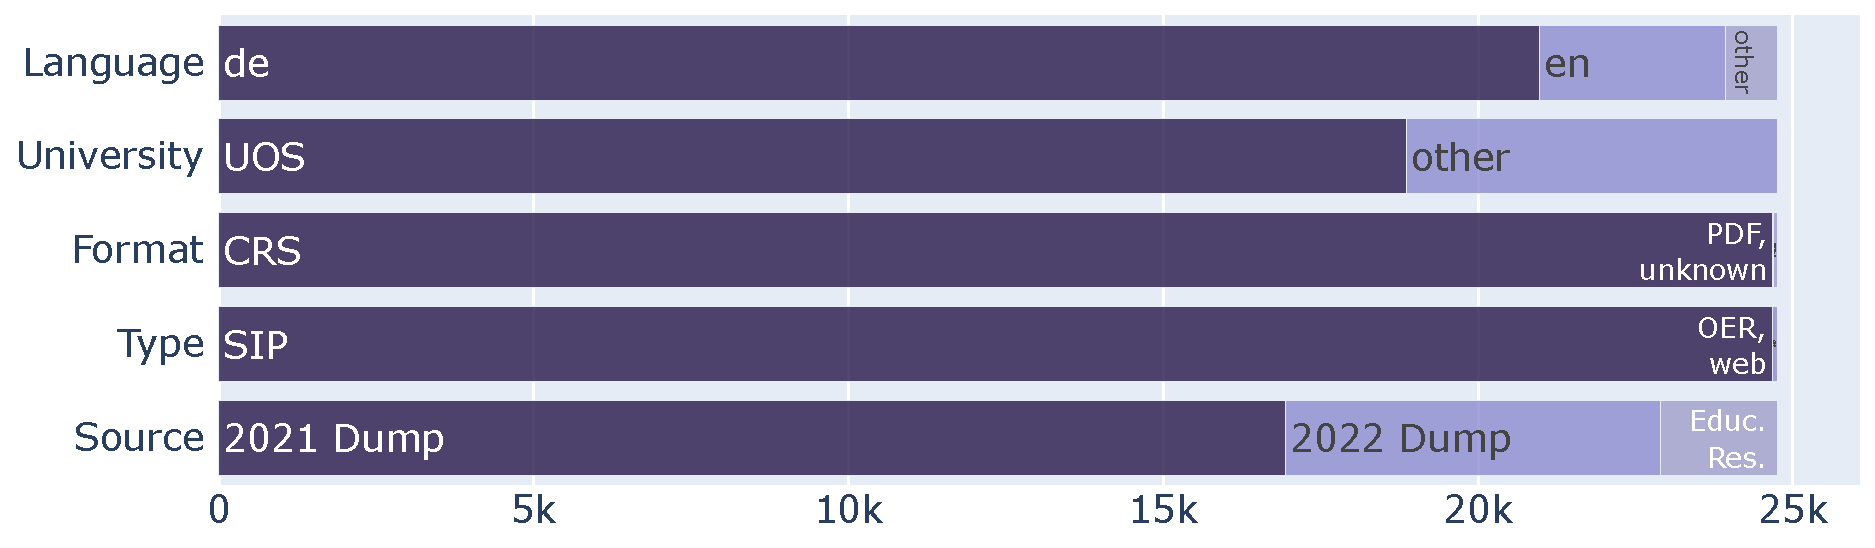
\includegraphics[width=1.15\textwidth,center]{graphics/dataset_new/statistics_bars.pdf}
	\caption{Different statistics of the SIDDATA-dataset}
	\label{fig:sid_statistics}
\end{figure}


\begin{figure}[H]
	\centering
	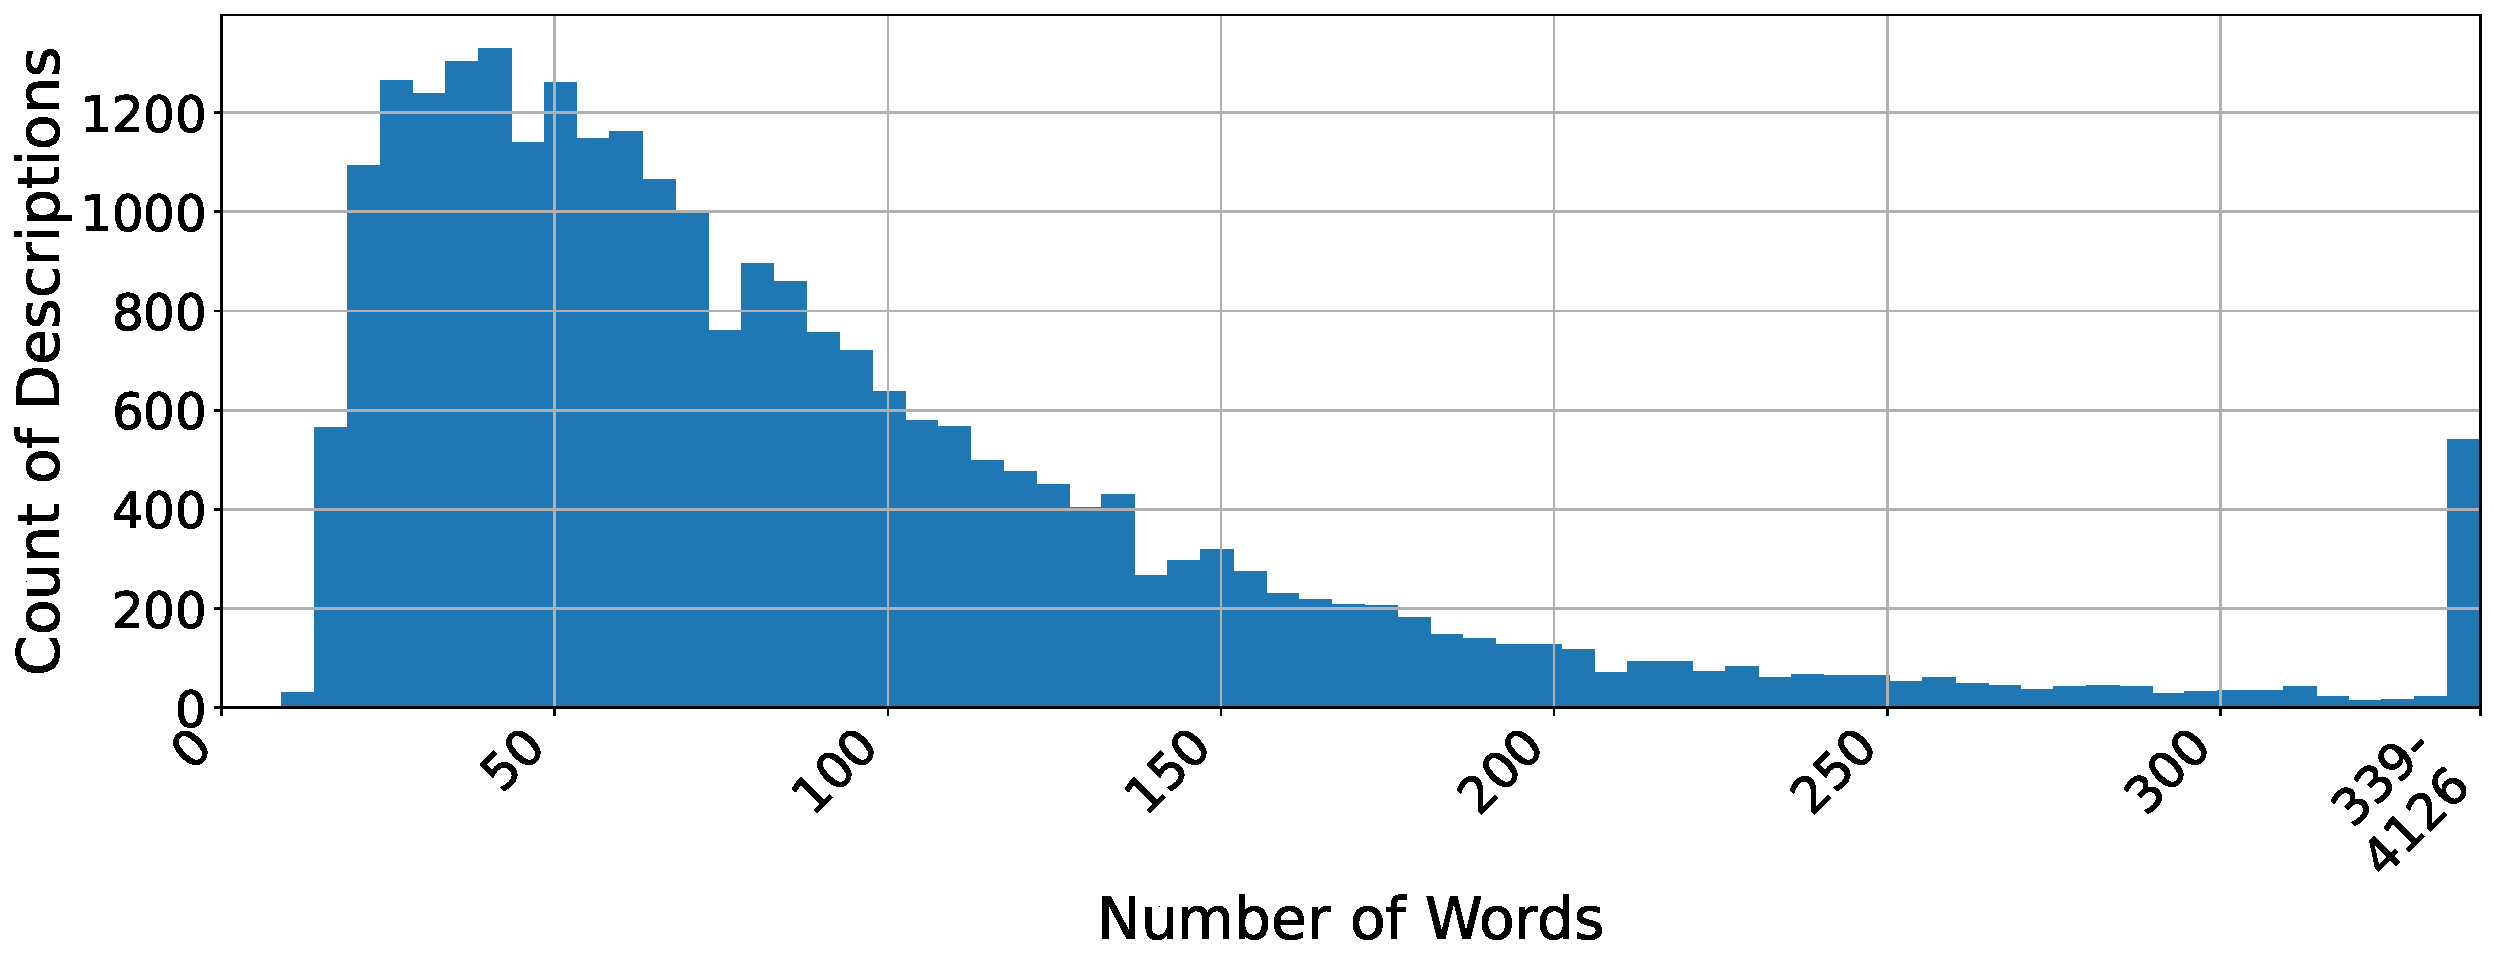
\includegraphics[width=0.95\textwidth]{graphics/dataset_new/words_per_desc.pdf}
	\caption{Words per Description for SIDDATA}
	\label{fig:sid_wordsperdesc}
\end{figure}


\subsection{Place-Types}

Because the SIDDATA-dataset differs in many regards from the datasets used in \mainalgos, %AS stated above (in siddta-section, in the first part of datasecs-section, in workflow-section, ...)
it does make sense to compare the results of the given pipeline on that dataset to the results of \mainalgos. To be able to compare the results achieved here with theirs, one of the datasets used by all of their papers was considered as well. Comparing on a original dataset also has the benefit of allowing to sanity-check if the implenetation is correct. If the performance achieved on this dataset is comparable to the performances of \mainalgos whereas the peformance for the SIDDATA-dataset is considerably worse, there is strong indication that the quality or quantity of the dataset is worse, suboptimal results on this one however would give indication that suboptimal results are the result of a faulty implementation.

There are two datasets used by all three authors: place-types and movie-reviews (see \autoref{tab:all_datasets}). Both of the datasets are available in preprocessed form\footnote{\url{https://www.cs.cf.ac.uk/semanticspaces/}} \cite{Derrac2015}. It was originally planned to use both of the datasets as basis for comparison, however unfortunately it is impossible to recover the form of it as originally used by \textcite{Derrac2015}: The original texts of the reviews are not available, but only their respective bag-of-1-grams (\glsentrylong{bow}) - even though the authors explicitly state that they worked with variable-length-n-grams. Even though the provided list of \glspl{cand} contains \glspl{ngram}, it is impossible to recover which of the \glspl{entity} contained it. While the algorithm can still be run only for the 1-grams, the results are not comparable with the original ones anymore\footnote{As all of the \mainalgos share an author, it is assumed that \cite{Alshaikh2020,Ager2018} had access to the full version of the dataset and did not share the stated problem.}.


\subsection{Other Datasets}

\section{Algorithm}

Let us finally go into detail about the main algorithm. The implementation of this thesis replicates and extends the algorithm proposed by \textcite{Derrac2015} with some novel contributions to deal with the given dataset. Further, some improvements from the works of \textcite{Ager2018} and \textcite{Alshaikh2020} are incorporated, who also replicated and improved the original algorithm and published together with Prof. Steven Schokaert. According to our evaluation of the field, these two papers provide some useful improvements in several aspects, as they apply the algorithm to different datasets, suggest more straight-forward ways of evaluating their performance, and help in understanding important concepts. That we are focusing on only those three papers should by no means imply that they are the only ones that were considered and influcenced this implementation,\footnote{See \autoref{sec:otherwork}} however in contrast to the other pertinent literature these two works do not substantially divert from the algorithm's core principles.
% see \autoref{sec:otherwork} - \cite{VISR12} and their tag genome, the fact that the algorithm detailed here is basically only one step in \cite{Alshaikh2019}, Gärdenfors himself suggested that one may use self-organizing maps instead of classical AI/NLP algorithms.

It is important to keep in mind that the algorithm is no rigid monolith but modularly consists of several components, such as \textit{dimensionality reduction}. Many of these components do not require specific algorithms, and \mainalgos also experiment with different components. The exact system for these components may be exchanged, and in the following these exchangeable algorithms are also referred to as hyperparameters. Note further that while this thesis mostly replicates the work of \textcite{Derrac2015}, the following will describe the algorithm as implemented here, which differs in some details from the original work. For the sake of clarity, very specific implementation details will be left out in the following description, as however reproducibility is an important aim for us, implementation details are available in Appendix~\ref{AppendixB} and linked where relevant. %\todoparagraph{Further, there is a table that compares the implementations here and in mainalgos, as well as another table what-configs-are-available where, the config-yamls and a section on what-other-things-could-one-have-done-hereandthere.}

\subsection*{Core Algorithm}

%\todoparagraph{The following explanation assumes that we accept some things as given. For now we'll do that, but we will later revisit and critically question many of these assumptions!}

% The core idea of the algorithm is to unsupervisedly find a a set of features which can be modelled as directions for a vector-space representation of the respetive entities.
The main goal of the algorithm is to unsupervisedly use text-corpora associated with the considered \glspl{entity}\footnote{From now on, the term \textit{\glspl{entity}} refers to the sample described by one text from the corpus (description, concatenated reviews, ...) from a certain domain. The corpus accordingly defines the domain: educational resources, movies, ...} to embed these into a vector-space where the axes correspond to human concepts/properties.\footnote{\textit{Concepts} and \textit{Properties} explicitly refer to what is defined in Criterions C and P, see \ref{sec:csdefinition}} This is referred to as \textit{feature-based} representation: A high-dimensional vector that numerically encodes the degree (\textit{protoypicality}) to which the entity corresponds to a number of appropriate dimensions. This is generally referred to as Conceptual Space and can be used as basis for explainable reasoning.

The general idea to achieve that is as follows: First, the entities are embedded as fixed-dimensional vectors. To allow for the types of reasoning from \autoref{sec:cs_reasoning}, it is embedded into metric spaces where the concepts of direction and distance are well-defined. \gencite{Derrac2015} original algorithm uses MDS (see \ref{sec:mds}) for this matter, which enforces metric distances. \cite{Ager2018,Alshaikh2020} both soften this requirement and also use document embedding techniques such as \gls{doc2vec} and averaged GloVe \cite{pennington2014glove} embeddings.

Additionally, words or phrases from the text are extracted as candidates for the names of the semantic dimensions. The underlying assumption is that \q{words describing semantically meaningful features can be identified by learning for each candidate word $w$ a linear classifier which separates the embeddings of entities that have $w$ in their description from the others} \cite[3574]{Alshaikh2020}: The better the performance of that classifier according to a chosen metric, the more evidence there is that $w$ describes a semantically meaningful feature. 
% * from Alshaikh2020: "Their core assumption is that words describing semantically meaningful features can be identified by learning for each candi- date word w a linear classifier which separates the embeddings of entities that have w in their description from the others. The performance of the classifier for w then tells us to what extent w describes a semantically meaningful feature"
In a final step, the candidate-words are clustered according to their similarity to find a fixed set of \emph{semantic directions}. A representative term for the directions is selected as dimension name, and the entities are re-embedded into a new space comprised of these dimensions, where the individual vector-components correspond to the ranking of an entity with respect to these dimensions.

The rest of this section goes into further detail for each of the individual algorithm components. \removeMe{An overview of which of the considered literature supports each components is given in \autoref{tab:compared_algos}.} Further, configuration files to enable exactly the respective components of the papers \mainalgos for the codebase of this thesis are listed in \aref{ap:yamls_for_origalgos}.

\todoparagraph{but before that, ager and alshaikh}

\removeMe{
\subsection{Regarding ager and alshaikh}

\todoparagraph{describe shortly what the improvements from [2,3] were}

\todoparagraph{Dass die den Zwischenschritt mit dem ganzen geeometric reasoning auf dem interim space nicht machen und DESWEGEN die requirement mit MDS soften konnen}

In principle Derrac2015, but with some components from Ager2018 and Alshaikh2020 as well as some own stuff. We will testi some claims or nonclaims of \mainalgos, bspw nutzen sie immer PPMI ohne je tf-idf zu testen. Also of course different nature of the dataset - their "how does this dimension correspond to the count in the reviews" doesn't make sense (their success-metric for the SVM is tailored to the one property, so we expect that one to be worse). We will elaborate on different ways to deal with that later.
}

\subsection{Algorithm Steps}
\label{sec:algorithm_steps}

% The core idea of the algorithm is to (unsupervised, data-driven) find a a set of features which can be modelled as directions for a vector-space representation of the respective entities. For that, the steps are:

This section describes the steps how to create an interpretable vector-space from the text corpus in detail. For that, we will explicitly elaborate on the parameter choices that branch up at every step for this specific implementation. %Note that absolutely is a combinatorical explosion it is impossible to try out all. %Further, this is about how this specific implementation does it, which may differ in some details from \mainalgos.

\label{sec:algorithmsteps}
\begin{enumerate}
	\item[\saveref{sec:algo_preproc}{1.}] \textbf{Preprocess} the corpus with default techniques and create a \textit{Bag-of-ngrams representation} (\ref{sec:techniques:bow}) of the texts.
	\item[\saveref{sec:extract_cands}{2.}] \textbf{Extract Candidate Feature Names} from words/\glspl{ngram} of the corpus.
	\item[\saveref{sec:generate_vectorspaces}{3.}] \textbf{Embed all Entities} into a fixed-dimensional vector space with demanded properties that captures the respective semantics.
	\item[\saveref{sec:svm_filter_cands}{4.}] \textbf{Filter Candiate Features} by training a linear classifier for each candidate that seperates the vector representations of the entities that contain the term from those that do not. If a specified metric for this classifier is sufficiently high, assume that the candidate term captures a \textit{salient} feature - its direction is then characterized by the orthogonal of the classifier's separatrix.
	\item[\saveref{sec:algo:cluster}{5.}] \textbf{Cluster/Merge the candidates} and calculate the feature direction for each cluster from its components, and (optionally) find a representative cluster-name.
	\item[\saveref{sec:algo:postprocess}{6.}] (optionally) \textbf{Post-process} the candidate-clusters.
	\item[\saveref{sec:algo:reembed}{7.}] \textbf{Re-embed the entities} into a space of semantic directions by calculating their distance to each of the feature direction separatrices.	
\end{enumerate}

This techniques first embeds the collection of texts into a  vector space, to afterwards extract important features from this space using linear classifiers. The second step is an original idea of \cite{Derrac2015}, however creating vector space embeddings from texts is a very popular technique, used for many tasks in \gls{nlp} \cite{Mikolov:Regularities,Mikolov2013a,Guo,Lowe,Turney2010}. This implementation relies on classical creation of the \gls{vsm}, for which the general creation process was explained in \autoref{sec:vsm_construction}. The steps \textit{Build the Frequency Matrix}, \textit{Transform Raw Frequency Counts} and \textit{Smooth the Frequency Matrix} are squashed into the preprocessing and embedding of entities. When \textit{extracing candidate features}, their frequencies must additionally be quantified - which may differ from the quantification when \textit{embedding all entities}.

An explicit and simple implementation compliant with each step could be a simple word tokenization and count to generate a bag-of-words (step 1) where each sufficiently frequent word is used as candidate (step 2). A \gls{dissimmat} of the individual \gls{bow}-vectors is compressed using MDS (step 3). A \gls{svm} calculates the accuracy for each candidate (step 4), and k-means-clustering on the 500 top-scoring terms subsequently creates 100 clusters and averages their directions (step 5). The distance to each of the hyperplanes is calculated (step 6), yielding new space for the entities. The sequence of steps is also given as pseudocode in \autoref{ap:algorithm_pseudo}. 
 
 The distinction of steps is not always this rigid: Instead of creating a dissimilarity matrix followed by dimensionality reduction, \cite{Ager2018,Alshaikh2020} use neural word or document embeddings.\footnote{see \autoref{sec:embeddings}} %Instead of extracing candidates from corpus tokens and training a linear classifier for each of them and use their orthogonal as direction, techniques such as LSA or LDA can be employed to find topic vectors directly. 
 We will come back to other ideas ideas when discussing future research opportunities (\autoref{sec:futurework}) by listing what other ways of fulfilling each respective step could have been considered.

\autoref{fig:dependency_graph} shows an automatically exported dependency-graph, displaying the individual steps of the algorithm as done in the accompaning code, also showing where selected important parameters are first used. As explained in \autoref{sec:architecture}, the modularity of the provided architecture allows individual components to be exchanged as needed and run in parallel.


\begin{figure}[h]
	\begin{center}
	  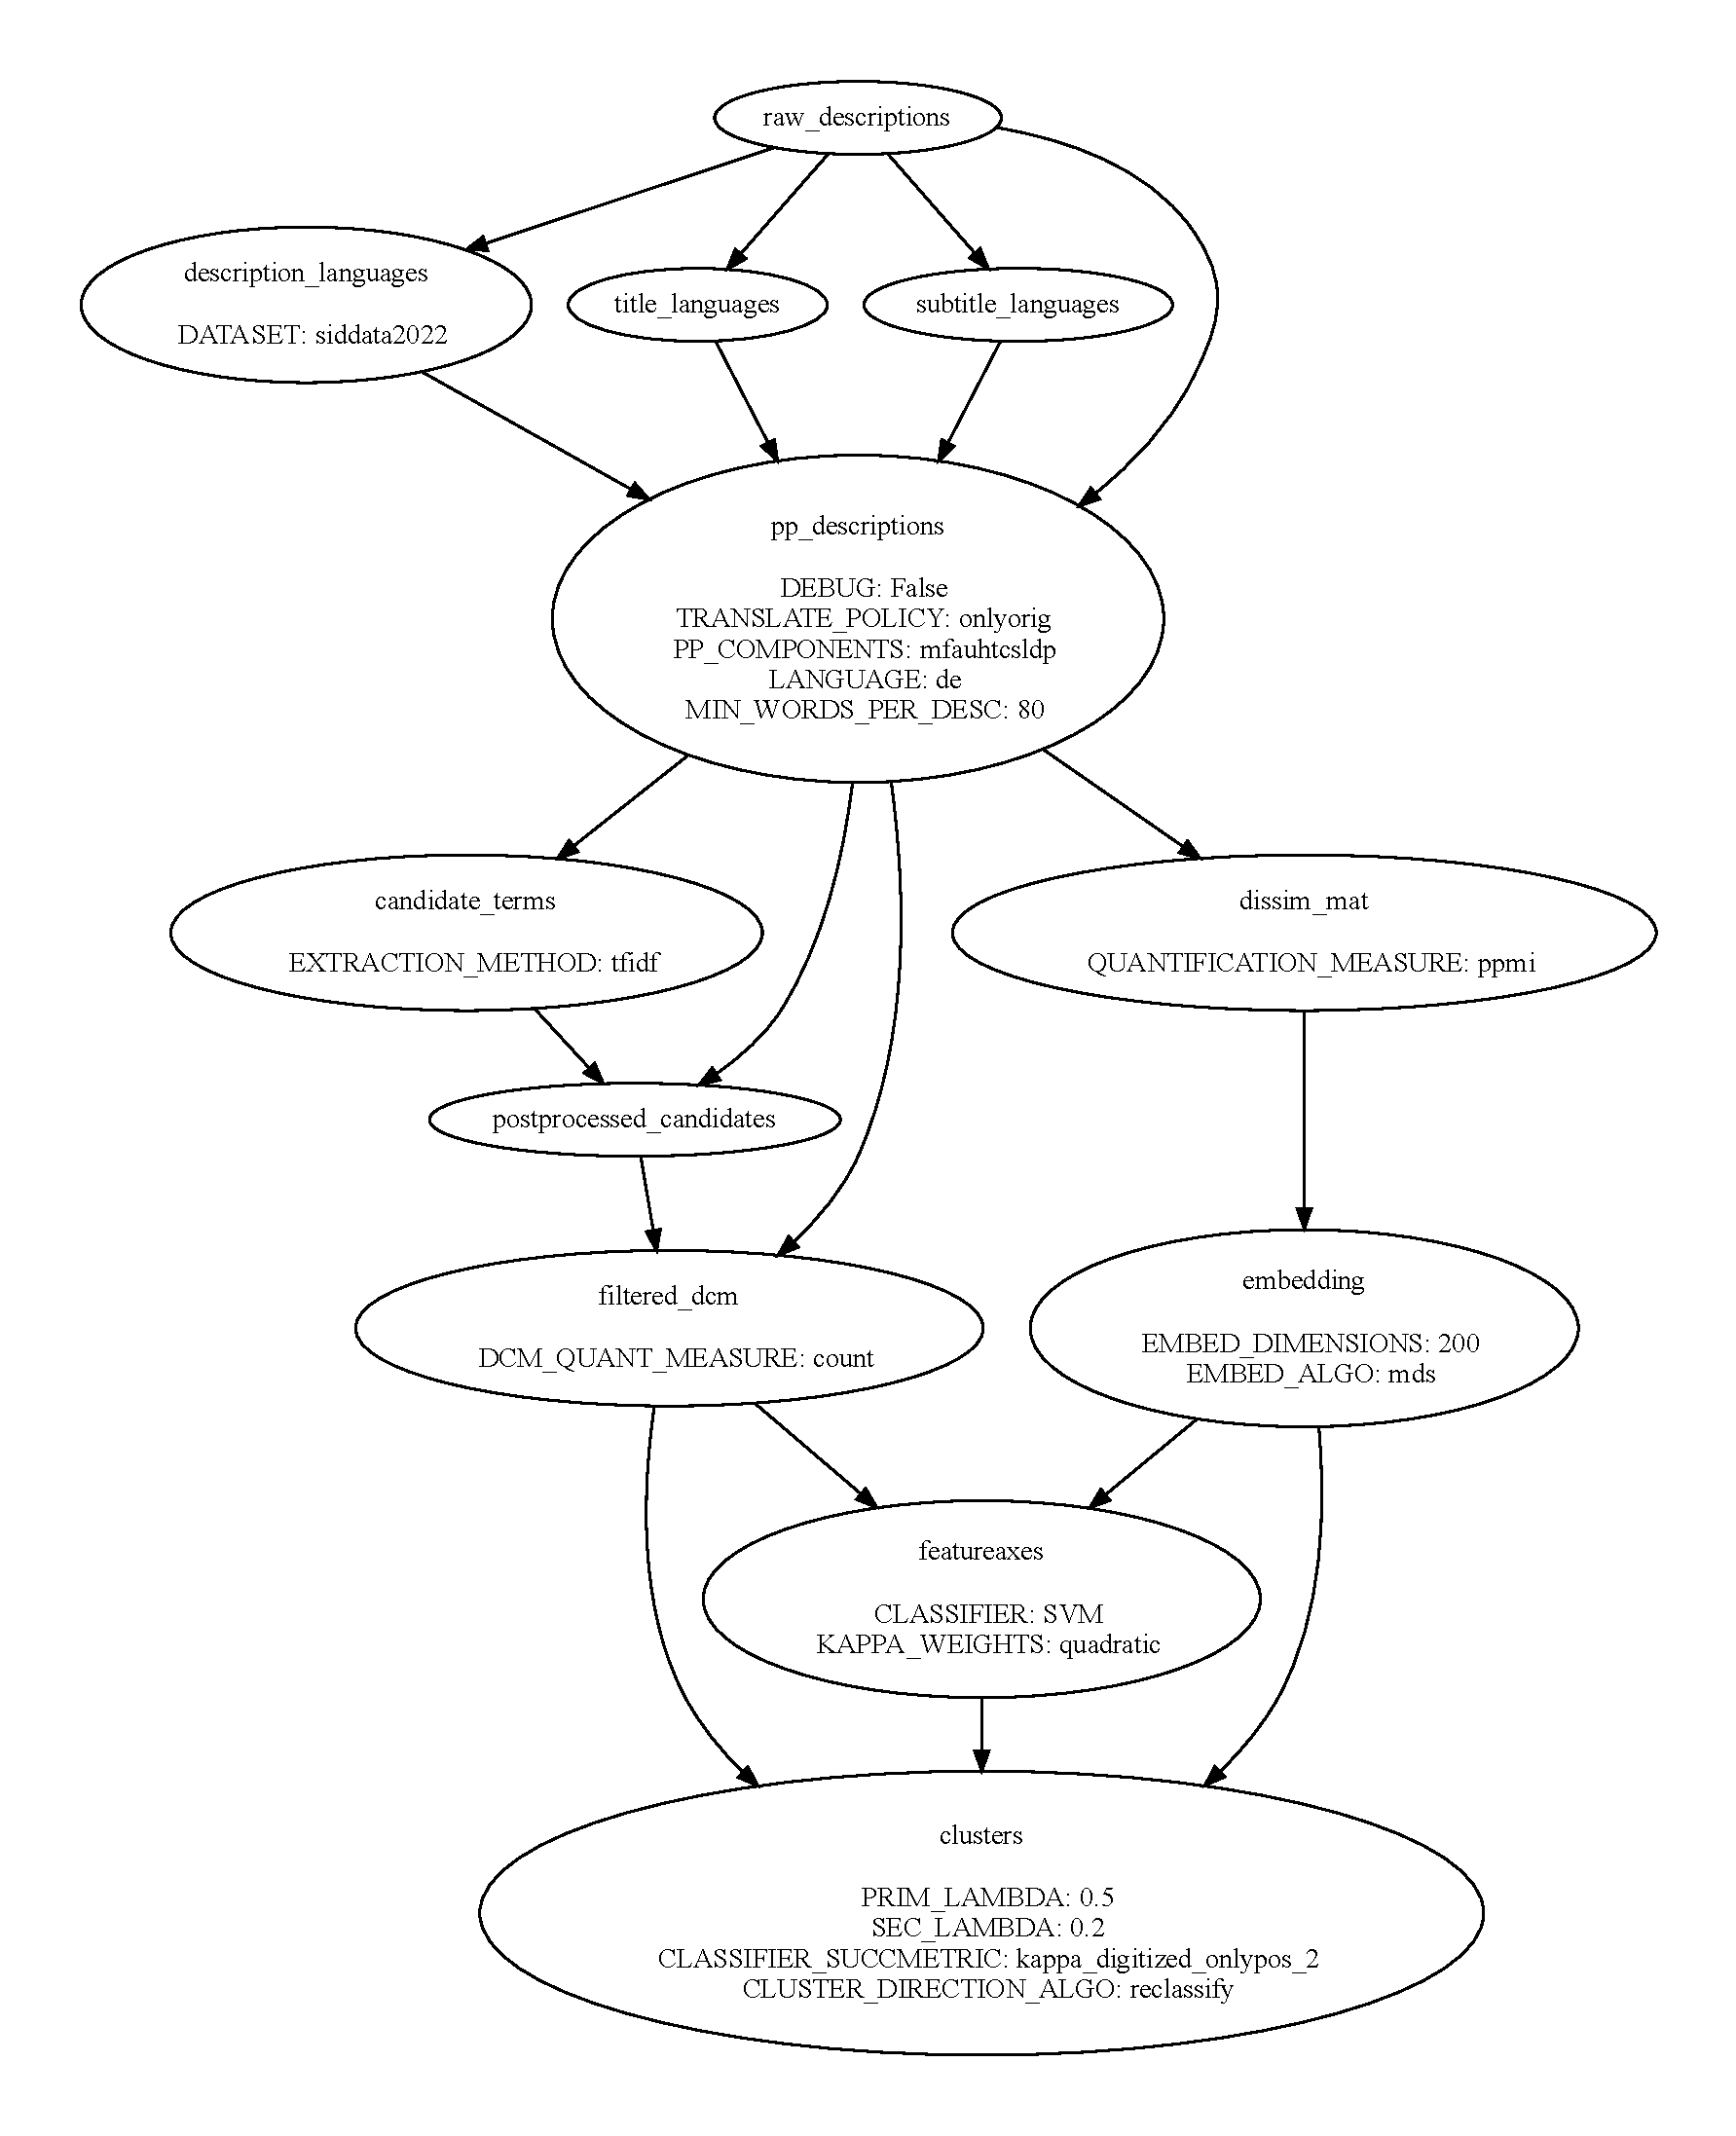
\includegraphics[width=0.9\textwidth]{dependency_graph.pdf}
	  \caption[Dependency-graph of the implementation]{Dependency-graph of the implementation, displaying the individual steps of the algorithm as well as their dependencies and where selected important parameters are first used. \todoparagraph{Generated using command XYZ}}
	  \label{fig:dependency_graph}
	\end{center}
\end{figure}


\subsubsection{Preprocessing\arrowref{sec:algorithmsteps}}

\label{sec:algo_preproc}

Before looking at the steps in turn, it should be noted that even the preprocessing does not work on completely raw data, but on curated and processed corpora. This processing is however not considered part of the algorithm, as it is very specific to the respective datasets and manual dataset exploration, tweaking settings such that they are best for each corpus separately. The preprocessing for the Siddata-dataset is described in \autoref{sec:dataset_siddata} and its implementation is done in separate Jupyter Notebooks.\footnote{Such as \url{https://github.com/cstenkamp/derive_conceptualspaces/blob/main/notebooks/create_datasets/Preprocess_Siddata2022.ipynb}} In the considered literature, the preprocessing is not considered part of the algorithm at all. Their implementations start from already fully processed datasets available as bag-of-words, each separately processed. Details of their individual processing per dataset is listed in \autoref{tab:all_datasets}. By incorporating the preprocessing into the pipeline, this work aims to increase adaptability and reproducibility, and also allows to experiment with different techniques such as translation or lemmatization or how duplicate entities with different associated texts are merged.
% In course-descriptions, I want some parts of the pre-preprocessing be part of the pipeline, like how we merge descriptions of different iterations of the same course that overlap to a high degree (sentwise-merge vs relative-term-frequencies)


A common prerequisit for NLP algorithms is to pre-process the text corpus. The preprocessing itself consists of multiple independent components chained after each other. Which components are necessary also depends on the processed dataset - as for example the \emph{placetypes}-dataset consists of a collection of \textit{tags} instead of full sentences, tokenising sentences or removing \glspl{stopword} becomes irrelevant. Other datasets may require additional cleaning or are already available in preprocessed form.

\paragraph{Translation} As the main considered dataset of university-courses is highly multilingual (see \autoref{fig:sid_statistics}), one of the first questions that needs to be addressed is how entities of different languages are handled. The algorithm consists of classical language processing algorithms such as comparing \gls{bow} representation of the entities, which means that the same text in two different languages may result in maximally different representations (see \autoref{sec:techniques:bow}). Because of this, before any other processing, the languages of each entity is checked, such that those of languages other than the demanded may be either translated, left out or used anyway. For details about the translation, it is referred to Appendix \ref{ap:translating}.\footnote{It should be noted that professional automatic translation is costly and thus not all texts are available in all languages.}

\paragraph{Components} The following components are developed for the preprocessing, every one of which can be individually enabled or disabled:

\begin{itemize}
	\item Prepend title and/or subtitle to the entities' associated text \itemtext{useful for the Siddata-Dataset, as the titles are often quite long and more descriptive than their descriptions}
	\item Remove HTML-Tags from texts 
	\itemtext{useful for the Siddata-dataset, as it includes descriptions for \glspl{mooc} which are crawled from websites and often contain such}
	\item Tokenise sentences 
	\itemtext{such that \glspl{ngram} across sentences are not considered}
	\item Lower-case all words
	\itemtext{reduces the amount of individual words and ensures that words at the beginning of sentences are mapped correctly}
	\item Remove stop-words / frequent phrases
	\item Tokenise words
	\itemtext{means splitting at the word-boundary, resulting in a list of words. Order must be kept in case n-grams are to be extracted.}
	\item \Gls{lemma}tize words
	\item Remove diacritics
	\itemtext{\emph{Diacritics} are glyphs added to basic letters, such as accents or German \emph{Umlaute}. Removing them converts for example the letter \emph{ä} to an \emph{a}}
	\item Remove punctuation 
\end{itemize}

The above can be done either be done with proprietary code for all of these steps,\footnote{Mostly relying on the python package \emph{nltk} \cite{bird2009natural}} or using \codeother{sklearn}\footnote{\url{https://scikit-learn.org/stable/}}s \codeother{CountVectorizer} (which is faster, but less configurable), as \cite{Ager2018} claim to have done.

\paragraph{On Stop-Words}
Removing stop-words from the texts is useful because it makes the resulting frequency more compact and thus less computationally intensive, and stop-words generally have very discriminative power, meaning their occurence among the entities is arbitrary, just making hte emeddings more noisy (cf. \autoref{sec:word_count_techniques}). There are however reasons to not remove them: Two words that are considered stop-words may posess relevant semantic content (such as a \textsc{Fällt aus} in a course title), and stopwordslists are often incomplete and of low quality \cite{nothman-etal-2018-stop}. For these reasons it is also possible to instead remove \glspl{ngram} that exceeded a certain frequency (\gls{df}).

\paragraph{On Lemmatization}
The languages most prevalent in the considered datasets are considered \textit{agglomerative}, which means word stems are changed by the addition of affixes and suffixes. Consequently, the same word may be present in multiple different forms, which modelled as completely dissimilar vectors in the present \glspl{bow}-approach. Lemmatization is the process of mapping different forms of these words onto the same stem. Considering that the Siddata-dataset consists of far fewer words than the others, this has important implications. For the german descriptions, this implementation relies on the \textit{HanTa} lemmatizer \cite{Wartena2020}.\footnote{\url{https://textmining.wp.hs-hannover.de/Preprocessing.html\#Lemmatisierung}}

The result of this step is a bag-of-ngrams representation for each entity (see \autoref{sec:techniques:bow}).


\subsubsection{Extract Candidates\arrowref{sec:algorithmsteps}}
\label{sec:extract_cands}
% Section 4.2.1 of Derrac2015

The final result of the algorithm is a metric space in which the individual dimensions (\emph{\glspl{feature}}/\emph{interpretable directions}) correspond to natural-language concepts and attributes. The candidates for these features are verbatim phrases extracted from the text-corpus of the \glspl{entity}, which are subsequently filtered and merged as necessary.

In \gencite{Derrac2015} work, the selection of phrases to be extracted depends on the dataset: For placetypes-dataset, all sufficiently frequent\footnote{\label{fnote:cand_thresholds}The respective thresholds are listed in \autoref{tab:all_datasets} as ``candidate word threshold''.} 1-grams\footnote{Note that in the case of the placetypes dataset, a 1-gram corresponds to all merged words of a tag.} were considered. For the other two datasets, they applied a \gls{pos}-tagger that extracted all sufficiently frequent\footnoteref{fnote:cand_thresholds} \textbf{adjectives, nouns, adjective phrases} and \textbf{noun phrases}, assuming that adjectives would correspond to gradual properties (\eg \textit{violent, funny}) and nouns to topics (\eg the \textit{genre}) \cite[Sec. 4.2.1]{Derrac2015}. Also, the authors ensured that the number of extracted candidates for both datasets is roughly equal, getting around 20\,000 candidates for movies and placetypes.

% Their method depended on the dataset - as their placetypes-dataset was just a collection of tags and the number of tags with term-freq >= XYZ (docfreq>2?! hä?) corresponded to their desired number of candidates anyway (around 22k), they just took all of these as candidates. For their movie-reviews-dataset, they considered all nouns, adjectives, nounphrases 	and adjective-phrases as detected by a POS-tagger. Doing something similar in the scope of this thesis led to suboptimal results, which is why alternative methods were developed
For this step, the implementation of this thesis differs from the original algorithm, as both taking all words as candidate and running a \gls{pos}-tagger led to suboptimal results in previous experiments, which indicated that the robustness of the algorithm is increased if less candidates are considered in earlier steps. \todoparagraph{This will be further argued and elaborated in the discussion.} To ensure comparability to these works however, in the case of the placetypes-dataset the original method of taking all words with a term-frequency of at least 50 was used. Similar techniques for the Siddata-dataset were also considered, but in constrast to the placetypes-dataset it is also important to consider various-length n-grams. 

% \todoparagraph{thing is I have less words but the algorithm seems to profit from less words as that makes it more robust}
% I would however argue that the difference here doesn't make a relevant difference 

In our implementation the candidate-extraction is split into four subsequently excecuted substeps, because depending on the algorithm used to extract the candidates the runtime of the individual components is comparably long and some settings are only relevant in later substeps. The steps are:
\begin{itemize}
	\item Extracting Candidate Terms
	\item Postprocessing the Candidates
	\item Creating the \gls{doctermmat} for the candidates and applying a \gls{quant}
\end{itemize}

As visualized in \autoref{fig:dependency_graph}, these substeps only depend on the preprocessed descriptions, which means they can be run in parallel to the creation of the embedding if \eg running on compute clusters.

% This can be done either based on the frequency (meaning all terms with a minimal term-frequency), based on some notion of *importance* (based on scores like tf-idf or ppmi), or by more complex means of figuring out *important* keywords and keyphrases. An example of the latter would be KeyBERT
Three main techniques are implemented to extract candidates from the text-corpus. Irrespective of the algorithm, only words with a sufficiently high \gls{df} are extracted, which is important to ensure that the classifier that determines its meaningfulness has enough samples in both clases. This means that the minimal freqeuncy can be calculated from the dataset size: In \cite{Derrac2015}, the minimal frequency for the movies-dataset with 15\,000 entities was only 100, meaning that the algorithm even works if only 0.6\% of samples are in the positive class. 


\begin{description}
	\item[By frequency:] consider all phrases that exceed a specified document-frequency (like \cite{Derrac2015}).
	\item[By a \gls{quant}:] consider all phrases that are prominent by some notion of \textit{importance} , such as the \gls{ppmi} or \gls{tf-idf}-score. Note that the respective scores depend on the combination of document and term, such that candidates may be extracted for some documents. Of course, all their occurences are considered in the creation of the frequncy matrix.
	\item[Using \emph{KeyBERT}\cite{grootendorst2020keybert}:] consider phrases whose BERT-embedding \cite{Devlin2019} is most similar to the text they are in. 
\end{description}

Using KeyBERT results in candidate terms that are most appealing in qualitative inspection, however it is also most computational demanding, techniques and requires substantial amounts of post-processing for the resulting phrases. More details on KeyBERT and how it is incorporated into the algorithm are given in the implementation are given in Appendix~\ref{ap:details_keybert}

Finally, a \gls{doctermmat} is created from the postprocessed candidates, containing the frequency for each candidate-phrase in each entity. The creation of this frequency matrix mirrors the process described in \autoref{sec:vsm_construction}, however only for the extracted words. After filtering this matrix to ensure that only candidates with a minimal \gls{df} or \textit{stf} are considered, a quantification is applied as described in \autoref{sec:word_count_techniques}. Available Quantifications include raw count, binarization\footnote{meaning all counts are either one or zero. According to \textcite{Alshaikh2020} this improves performance, however we could not confirm this.}, tf-idf or PPMI. We expect that expressing the relation of terms and documents by something else than the raw count will prove especailly useful for the Siddata-dataset: As it does not consist of concatenated reviews but short descriptions, each individual word will only occur a few times per description. Because of that, a \gls{rank} induced from the count will be not very meaningful when later comparing it to the ranking induced by the classifier.

\subsubsection{Generating Vector Space Embeddings\arrowref{sec:algorithmsteps}}
\label{sec:generate_vectorspaces}

In this step, the individual \glspl{entity} are embedded into a fixed-dimensional vector space, making up a \emph{frequency matrix}.\footnote{The previous step already created a frequency matrix that encodes the relevance of a candidate-phrase for each entity- this is a spearate one that later serves to encode each document as a vector} Neither this nor the frequency matrix from the previous step will used to finally calculate similarities on, but both are interim results to get the dimensions necessary for these similarities.

% Importantly, while this matrix is a \gls{doctermmat}, it is only an interim result in the algorithm and the calculation of distances and directions will be done on another matrix from a later step. %This is where our pipeline starts to diverge from what the pipeline specified in \nameparanref{sec:vsm_construction}.  in the previous step, and in this step we create another one that encodes each document as a vector. 

Embedding words, \glspl{ngram}/phrases or other tokens, as depicted by \cite{Turney2010,Lowe}, generally involves counting the token frequencies, transforming them to get relative frequencies, and performing dimensionality reduction on the resulting matrix.

So far (step 1), we have counted the token frequencies. \textcite{Derrac2015} argued that this space must be Euclidean, such that geometric/algebraic solutions correspond to commonsense reasoning tasks (see \autoref{sec:reasoning}). Another requirement is that the number of dimensions is be chosen as hyperparameter to the algorithm to be able to find a compromise between compression and expressive power. Because of these two requirements, they selected \gls{mds} for dimensionality reduction.

As stated in \autoref{sec:mds}, \gls{mds} calculcates a Euclidean \gls{vsm} from a set of pairwise distances. This means that the algorithm first creates a \textit{Dissimilarity Matrix} that encodes the distance between all pairs of entities (represented as Bag-of-ngrams representation), from which subsequently the final embedding is generated. 

In this implementation, the dissimilarity matrix is created using distance metrics for the quantified bags-of-ngrams of the respective entities. Note that this quantifiation does not need to be the same one as the one used for quantifying the relatedness of the extracted candidates and the documents.\footnote{As will be shown in the result, doing so sometimes even outperformed other configurations.}

\paragraph{Document embeddings}
If the strict requirement for a metric space is dropped however, many different algorithms may instead be used at this point - not only different dimensionality reduction methods for the embedding, but also ones that do not rely on the distance matrix or even the \gls{bow} at all, like document-embedding-techniques such as \gls{doc2vec} \cite{Le2014} (as \eg used by \cite{Alshaikh2020}). This would not require the count of token frequencies followed by a \gls{quant}, but not affect the rest of the algorithm. As, however, document embeddings tend to be created on the basis of \gls{cos}, this will not result in a Euclidean metric. \textcite{Alshaikh2020} experimented with this, however it performed worse than the original algorithm relying on MDS (see \autoref{tab:f1_placetypes_long}), which is why this technique was not futher pursued in this work.

\paragraph{Classical Processing}
The default way of doing it is, however, to create frequency matrix counting the token frequencies of each word of an entity and using a \gls{quant} to transform these raw counts. In this implementation, the \gls{dissimmat} that is required for the MDS-algorithm created on basis of the \emph{normalized angular distances} of the \glspl{bow} of the respective entities, which is relates to the \gls{cos} and is defined by \textcite{Derrac2015} as:

\vspace{-5ex}
\begin{align}
	ang(e_i, e_j) &= \frac{2}{\pi} * \arccos \left( \frac{\vec[m]{v_{e_i}} * \vec[m]{v_{e_j}}} { \lVert \vec[m]{v_{e_i}} \rVert * \lVert \vec[m]{v_{e_j}} \rVert }  \right)  \label{eq:norm_ang_dist} \\
	&= \frac{2}{\pi} * \arccos(1-\cos(\vec[m]{v_{e_i}},\vec[m]{v_{e_j}})) \nonumber
\end{align}

Finally, the dimensionality of the frequency matrix is reduced using the MDS-algorithm described in \autoref{sec:mds}. \cite{Derrac2015} also experiment with the \textit{Isomap} algorithm, which does not yield a Euclidean space but one of geodesic distances. As the results for their implementation are, however, of worse quality than those for MDS, it is not considered further in this work. 

In the publication of \textcite{Derrac2015}, the result of this embedding is used to experiment with the explainable classifiers (discussed in \autoref{sec:reasoning}). Due to the usage of MDS, this space has clearly defined concepts of \textit{betweeness} and \textit{parallesism} between the entities, however it is important to stress that it does not have interpretable dimensions and is, so far, a plain \gls{vsm} as described in \autoref{sec:vsm_construction}. 


\subsubsection{Filter Candidates by Classifier Performance\arrowref{sec:algorithmsteps}}
\label{sec:svm_filter_cands}

This step brings together the entity embeddings and the extracted keyphrases, to finally find semantically meaningful directions in the space the entities are embedded in. For that, classifiers are trained for all previously extracted candidates, each yielding a \textit{Candidate Feature Direction}, which are subsequently filtered to detect those corresponding to semantically meaningful features. The algorithm is executed separately for each candidate term and looks as follows:

All entities are split into two classes: Those that contain the respectively handled candidate term and those that do not. To quantify how well each candidate word captures semantic content of the entities, a linear classifier is trained to separate the embeddings of these two classes. The best example for such a classifier is a \gls{svm} which does not rely on the kernel trick. As visually exemplified in \autoref{fig:3d_hyperplane_ortho}, the result is a hyperplane that best divides the positive from the negative samples. Regardless of the dimensionality of the original space, this hyperplane has a one-dimensional orthogonal vector. Each of the entity-embeddings is subsequently orthogonally projected onto it. The distance of this projection to the plane offset\footnote{The coordinate where it crosses the decision surface} is a scalar that encodes the distance to this decision hyperplane. 

This distance encodes \textit{how much} this point is considered to be protoypical of the respective class by the classifier, for the positive as well as the negative class. Given that the original space is created based on similarity measures of the entities, the \textit{Bag-Words-Hypothesis} (\autoref{sec:bow_hypothesis}) states that similar words should have similar words - meaning maximally dissimilar entities are far apart from positive ones.\footnote{To stick with the example of movies, the assumption is that movies that are maximally unscary are maximally far from the away from scary ones: An entity that has a maximally dissimilar distribution of words than those that are \textit{scary} means a maximally maximally dissimilar movie, as little of its \textit{latent topics} (see \autoref{sec:lsi}) agrees with the scary ones: The more dissimilar, the less scary.} Because of this, the hyperplane's orthogonal can be considered an axis that encodes how much each entity agrees with the feature that is the basis of the classification. Accordingly, a ranking of the entities in terms of this distance should encode their degree of having the respective feature.

According to \textcite{Derrac2015}, the performance of this classification encodes how good a candidate serves as feature direction. This can be explained like this: As discussed earlier (\autoref{sec:word_count_techniques}), unimportant words are arbitrarily throughout the corpus. Due to distibutional semantics, topics that are very prominent in some texts but not in others will influence the position of a texts' embedding in the vector space more than \textit{unimportant} words, which do not signify a latent topic of the corpus. This means, they do not correlate with other words and do not explain much of the dissimilarity of the embeddings. Accordingly, unimportant words do not influence the positions of the entities' embedding other than being \textit{noise}. This randomness does not go along with a cluster of positions in any of the dimensions, as noise gets removed in process of dimensionality reduction. This makes it reasonable to assume that the a classifier can split entities that contain a word from those that do not, the more the word is an \textit{important topic} in the sense that it explains the dissimilarity in the entities.

Because of this, \cite{Derrac2015} henceforth only consider those terms as \textit{faithful directions} that explain a lot for variance in the data whose performance exceeds a certain threshold.\footnote{\q{if this classifier is sufficiently accurate, it must mean that whether word w relates to object o (i.e. whether it is used in the description of o) is important enough to affect the semantic space representation of o. In such a case, it seems reasonable to assume that w describes an important feature for the given domain.} \cite{Ager2018}}

Concretely, the score used by \cite{Derrac2015} to assess the performance is not the accuracy or some other measure of the binary performance of the classifer, but rather if the ranking induced by the classifier corresponds to ranking of number of occurences\footnote{or the PPMI-score, the authers are imprecise in their wording - we will elaborate more on that later} of that word: The more these agree, the more we consider this direction \q{to be a faithful representation of the term} \cite[20]{Derrac2015}. The reasoning behind that becomes especially clear when considering the root of their datasets - in the case of reviews or tags it is the case that the more often a word is mentioned, the more relevant the word is for that entity. In the case of using a \gls{quant} such as the \gls{ppmi}-score, this instead becomes: The more salient relevant for this entity but not for the others the word is, the higher the score.

A score function compares these rankings, such that only those terms where the correspondance of these rankings exceeds a certain threshold are considered as candidate directions henceforth. For that, \textcite{Derrac2015} say that they use the Cohen's kappa, which is a metric to compare rankings that can deal with highly imbalanced data. Considering that for most candidates, most of the entities will be in the negative class this makes sense.\footnote{\textcite{Ager2018} compare the kappa-score to accuracy and argue that accuracy works better than the kappa-scores.} Unfortunately, the authors do not give many details on how this scoring is implemented. While \cite{Ager2018,Alshaikh2020} explicitly say that they are interested in the PPMI-scores\footnote{Though the uploaded code of \cite{Alshaikh2020} does not compare rankings but raw values}, from \cite{Derrac2015} it is not even clear if they take the count or the PPMI-score. As that is highly relevant, we try many different ways of this scoring and report them in the results. We also compare the overlaps of different kappa-scores to check if the choice is as imporant as we think it is. Which scores we used and how they are written here is listed in the implementation details: \autoref{tab:kappa_measures}.

Subsequently, only those candidates with high enough scores are considered, and the othogonals of the respective classifiers considered their respective \textit{candidate feature direction}, encoding the degree how much an entity corresponds to this feature. The number of features with a sufficiently high score can also serve as estimate of how good the parameter-combination so far was: if not enough well-scoring features were extracted, the final embedding which is created through only a subset of these features does not explain much of the original variability in the data.

\todoparagraph{Tpower0.5 etc in den Glossary!}

\subsubsection{Merging the extracted candidate-directions\arrowref{sec:algorithmsteps}}
\label{sec:algo:cluster}

The previous step yielded many \textit{basic feature directions} that are defined as direction of the orthogonal vector for the hyperplanes splitting each individual candidate \gls{ngram}. The performance-thresholds are set such that many more directions are generated than the demanded dimansionality of the final embedding, such that they must be clustered and merged.

This is done via the following substeps, each of whch will be closer eloaborated:

\begin{itemize}
	\item Cluster good-performing candidates by their similarity
	\item (optional) Remove uninformative features
	\item Recalulate the direction of the cluster
	\item (optional) Find a representative name for the cluster
\end{itemize}

\paragraph{Clustering the candidates}

Clustering refers to an unsupervised algorithm that groups items based on some notion of similarity. In our case the assumption is that semantically similar concepts have \textit{close} vectors, which is given due to the \gls{bow}-hypothesis that states that the underlying structure of our dataset is expressed by the usage of related words (\autoref{sec:bow_hypothesis}, \ref{sec:lsi}).\footnote{In case of the Siddata-dataset, it may mean that in courses that contain the word \textit{computer} have a high chance of also containing \textit{program}.} As these vectors in principle only encode a direction, their similarity can be calculated by their \gls{cos}.

The clustering should reduce the number of features and also ensure that the resulting directions are different enough. Note that unlike \eg in Principal Component Analysis (PCA), the suggested here techniques do not enforce orthogonality, such that the resulting directions may remain linearly dependent to a certain degree. As in the final embedding only the projection onto those directions is relevant, it must be ensured that enough of the data's original variation is covered by these directions. To ensure that, we follow \gencite{Derrac2015} suggestion to allow for redundancy by extracting twice as many directions than the original \gls{vsm} dimensionality. 

The following steps describe the implementation of the original clustering method of \textcite{Derrac2015}, also used in our work:

First, we consider the best \textit{basic features} as \textit{main directions}. For that, we select one of the scores calculated in the previous step and select all candidates that exceed a threshold (\cite{Derrac2015} suggest $\kappa \geq 0.5$).
To get the directions, we follow the following algoritm:

\vspace{-1ex}
\begingroup
\verbatimfont{\footnotesize}%
\begin{verbatim}
	greats = filter(candidates, 0.5)
	directions = greats.argmax()
	for nterm in range(ndims*2):
	  greats = set(greats)-set(directions)
	  distances = {cand: min(comparer(cand, compareto) 
	                for compareto in directions) 
	                  for cand in greats}
		directions.append(compares.argmax)
\end{verbatim}
\endgroup
\vspace{-1ex}

This starts with the best candidate and then iteratively adds the one from the set of top-scoring candidates that most dissimilar to the set of final directions. The result is a set of $ndims*2$ main directions, which are henceforth considered the Cluster centers. Subsequently, all leftover terms from $T^{0.5}$ as well as all terms from $T^{0.5}$ are added to the respective cluster whose direction they are most similar to. 

\textcite{Derrac2015} used the \gls{cos} to measure the respective similarities. This may lead to unexpected situations (discussed in \autoref{sec:discuss_points}). As alternative similarity metric that does not rely on the angle between their vectors, \cite{Alshaikh2019} suggest to use the overlap of the positive-samples of two features as similarity. This was however not yet implemented in this thesis.

Alternatively, to the described algorithm, is also possible to use the popular \textit{k-means} algorithm for clustering, as done by \cite{Ager2018}. We do not present results for this approach here however, as it lead to a substantial increase in runtime, without affecting performance much. In the development we also noticed that many clusters contain a lot of irrelevant terms. To alleviate this, we experimented with different techniques, for example setting minimal similarity thershold that must be given for a term to be added to a cluster, however so far no formal evaluation to test how this affects performance was performed.


\paragraph{Find Cluster-Direction}

So far, we have a set of clustered canidates terms, each of which has an individual direction. The final \textit{feature-direction} must subsequently be found from the elements of the cluster. For that, \cite{Derrac2015} and \cite{Ager2018} define the cluster centroids as the average of all (normalized) vectors per cluster. In our experiments, however, we noticed that the final direction tends to be too much affected by irrelevant cluster-elements. Because of this, we experimented with other techniques to determine the cluster direction. Other considered methods include \eg to 1. just consider the direction of the cluster-center, or 2. to weight the influcence of each cluster-element by their kappa-score.

The best performaning method however was the \textit{reclassify}-algorithm, which (similar to \cite{Alshaikh2020}) finds the cluster-direction by training a new classifier that splits those \glspl{entity} that contain \textit{any of the elements} from the cluster from those that do not, analogous to the previous step.\footnote{except that it requires to generate and quantify a new frequency matrix from the sums of the individual counts.}. Doing this however often leads to the opposite problem than the previous step, namely that for many clusters there are almost no entities that do not contain at least one of the cluster elements. To counter this, we instead trained a classifier to split the 30\% of entities with the highest \glspl{quant} from the 30\% of entities with the lowest \glspl{quant}. A comparison of this algorithm with the method of \cite{Derrac2015} is given in the Appendix as \autoref{tab:text_per_dim}. As \cite{Alshaikh2020} already performed formal experiments with this that have shown its superior performance, all generated results of this work rely on this algorithm. 

\paragraph{Bad Clusters}

After these steps, we finally have the vectors that correspond to semantic directions. However, as there were still clusters of uninformative terms, \textcite{Alshaikh2020} have an additional step to remove uninformative cluster. As this bases on another clustering algorithm used by the author (namely \textit{affinity propagation}) which does not allow to specify the number of clusters, it was not implemented in the scope of this thesis.

\paragraph{Find a representative Cluster Name}

An important advantage of the clustering process is that it makes the extracted directions more \textit{descriptive} due to the fact that they are described by several phrases instead of only one. However, it may be helpful for an attractive user interface to find the single \textit{best} description of the cluster direction by its element.

An analysis of \cite{Carmel2009} showed that a statistical method to extract features from clustered text corpora identified the labels of human annotators as one of the top five most important terms in only 15\% of cases, implying \q{that human labels are not necessarily significant from a statistical perspective} \cite[139]{Carmel2009}. In their paper, they suggest several methods to find one representative name for the cluster. 

\textcite{Derrac2015} and its follow-ups \cite{Ager2018,Alshaikh2020} did not care about such methods and instead use either the name of the cluster center as its description or the cluster center plus two other sample elements. This work experimented with several techniques to get a more representative direction name. One of these techniques used the KeyBERT-algorithm (see \autoref{ap:details_keybert}) to find the term that is most similar to the set of terms making up the cluster. We also experimented with a method that embeds the cluster terms using \gls{word2vec} and returns  the word behind the vector that is closest to their average, which is not neccessarily part of the original set of words. Similarly to \gls{lsa} (\autoref{sec:lsi}), it is also possible to consider the entity whose \textit{pseudo-document} embeddings is closest in direction to the cluster direction.

The best technique to find a cluster-name was not evaluated yet. All considered methods that formally evaluate the corresponding feature-directions work independently of the actual cluster name. This is unfortunate, because \textit{subjectively}, the name of the respective directions is very important for the usability of any recommendation engine based on this work. Especially this subjectivity indicates that the only way to evaluate the cluster-names is with a study of human subjects.

\todoparagraph{Kappa in den Glossary!!}

\subsubsection{Postprocessing the Feature-Directions\arrowref{sec:algorithmsteps}}
\label{sec:algo:postprocess}


The main contribution of \textcite{Ager2018} is a postprocessing step that changes the final space such that the ranking of entities \wrt each feature direction more closely mimics the ranking of frequencies of that direction's cluster words. The reasoning behind this is that the original embeddings from which the feature directions are created are based on global similarity. This makes it very vulnerable to outliers which often take up extreme positions. If one now creates the feature directions from the space, these outliers are assumed to have certain properties. The space is optimized for that, which limits the quality of feature directions in the space. The problem here is again the global similarity: If one entity ranks high for a feature, it is very likely that another entity that is close to that will also rank high for this feature, even though it may be something completely different. So to get better feature directions one has to distort the space. The authors accordingly again use the BoW representation of the entites to fine-tune the positions of the embeddings in the final space: After the clusters are collected and the entities re-embedded, for each feature a new ranking is computed by the summed frequency of any of a cluster's words per feature and entity. Each entity is thus represented as Bag-of-Clusters and again scored with PPMI to generate a ranking for each cluser/direction. This ranking is then used as a target for a simple \gls{ann} that distorts the space representation. As has been shown that it increases the algorithm performance only slightly while adding a substantial amount of work, it was not implemented in the scope of this thesis. 

\subsubsection{Re-Embedding the entities into the new space\arrowref{sec:algorithmsteps}}
\label{sec:algo:reembed}

To finally get the \textbf{feature-based representation} of the entities, they are re-embedded into a space where each of the vector components is a semantic directions and the value are the respective \gls{rank}ings. According to the authors, the degrees of similarity are not supposed to be encoded, which is why only the respetive ranking is considered.



% \subsection{Modifications from \textcite{Ager2018,Alshaikh2020}}

% \subsubsection{\textcite{Ager2018}}
% \label{sec:ager}


% \textcite{Alshaikh2020}

% \todo

% \removeMe{
% \subsection{Concluding stuff for algo}

% \subsection{Features and differences to original algorithm}

% \includeMD{pandoc_generated_latex/3_features_differences}

% \subsection{Reasonable params}

% \includeMD{pandoc_generated_latex/3_reasonableparams}

% \subsection{Algorithm Complexity}
% }


\section{Architecture}
\label{sec:architecture}

As elaborated in \autoref{sec:reproducibility}, one of the main motivations for this thesis was to create a publicly available \textit{open-source} version of the algorithm that is easily \textit{understood} and \textit{reproduced}, \textit{adaptable} for other datasets and methods, as well as fast and \textit{scalable}, meaning it can be run maximally efficient on single machines but also on compute clusters, such as the \acrshort{ikw} Grid.
%TODO: Hier schon eindeutig sagen dass es auf ner single machine infeasibly lange läuft und deswegen der ganze Bums fürs Grid nötig war!!

% Main goal: BETTER ARCHITECTURE. Most important things for that: scalability, modularity, transparency, reproducibility, understandability, objectiveness, systematicacy, sustainability, adaptability
% describing this because I want to encourage extending the code etc and for that not only the algorithm but also the architecture should be described 
% and I think that was successful: This codebase contains everything and finally fulfills code-standards! 

This section will outline the architecture that was developed in order to achieve the aforementioned results. The resulting pipeline is the result of a lot of trial-end-error, but fulfills all of the aformentioned criteria, dealing with vastly differing sizes and kinds of datasets, minimizing runtime wherever feasible and allowing for a multitude of parameters at every step of the process. %TODO: don't like this paragraph, lieber später nohcmal auf die design principles eingehen und sagen dass sie alle fulfilled sind.

The rest of this section will go into further detail regarding the architecture of the resulting code-base. \todoparagraph{it will start with xyz and then asdf and then yaddayadda}

\subsection{Implementation}

The associated program is written by the author of this work and licensed under the \emph{GNU General Public License} (GNU GPLv3). The source code is written in the Python Programming Language and available digitally on GitHub\footnote{Source code: \url{https://github.com/cstenkamp/derive_conceptualspaces/}\\Source of this Document: \url{https://github.com/cstenkamp/MastersThesisText/}\\Compiled Document: \url{https://nightly.link/cstenkamp/MastersThesisText/workflows/create_pdf_artifact/master/Thesis.zip}}. In order to ensure that no work after the deadline is considered, it is referred to the signed commits \todoparagraph{COMMIT} and \todoparagraph{COMMIT}. 

The code is a proper python-package that can be installed into any Python 3.10 environment using for example python's default package manager pip:\\ \mytokens{pip install git+https://github.com/cstenkamp/derive_conceptualspaces.git@main}~ .\\ It can then be run using \mytokens{python -m derive_conceptualspace <COMMAND>} \footnote{The command \mytokensfnote{python -m derive_conceptualspace --help} gives a peak into what sub-commands can be used}. For more information on how to invoke the code base with these commands it is referred to \autoref{ap:usecase_click}

To guarantee reusability of this code-base, there is also a \emph{Dockerfile}\footnote{{\url{https://github.com/cstenkamp/derive_conceptualspaces/blob/main/Dockerfile}}} that allows to easily create a \emph{Docker-Container\footnote{\url{https://www.docker.com/resources/what}}} from it\footnote{A Container can be thought of as a lightweight virtual operating system, in which the codebase is bundled together with all required dependencies, libraries and configurations, enabling users install this software on any system without having to download or install anything besides this container, irrespective of operating system or software versions on the host \acrshort{os}. For more info about the container, it is referred to \url{https://github.com/cstenkamp/derive_conceptualspaces/blob/main/doc/docker_intro.md}.}.

\subsection{Modularity}

The developed algorithm consists of clearly divisible components (as demonstrated in \autoref{fig:dependency_graph}), where the runtime for each of the steps is roughly in the same order of magnitude. All of the aforementioned (\autoref{sec:algorithm_steps}) steps are itself algorithms with many \gls{param} each. Furthermore, the framework described here does not even require particular algorithms for the individual components, but rather a classes of algorithms like \emph{dimensionality reduction techniques}. This means that in practice, there is a combinatorical explosion of settings and \glspl{param} that must be experimented with in order to find the best-performing one. Because of the clear modularity of the algorithm however, many of these become only relevant in a later step of the pipeline. Due to this, it is reasonable to make the architecture as modular as possible, storing interim results before every step, such that two parameter-combinations that differ only in \eg the fourth step of the pipeline can share the intermediate results up to that point, keeping the required computation to a minimum. 

The design principle of maximal modularity is the cornerstone of the developed pipeline. All of the interim results store the configurations that were required for the respective algorithm (and forward the ones of the input-files they transformed), as well as the created output and plots. When there are different possible algorithms for a step, it is ensured that its result are of the same format, as required by the next step. Many of the individual steps generate additional plots that can be used as sanity-checks to quickly inspect if the results so far are reasonable.

\subsubsection{Workflow Management}

A pipeline where multiple intermediate files for different parameter-combinations are created introduces the problem of \emph{dependency resolution}: Ultimately, there is supposed to be one final file for every combination. This file however relies on intermediate files, which in turn rely on intermediate files. To resolve these dependencies, there are many existing \textbf{Workflow Management Systems}. For this thesis, \textbf{Snakemake}\footnote{\url{https://snakemake.readthedocs.io/en/stable/}} \cite{Molder2021a} seemed the right choice.

Snakemake defines a small comprehensible domain-specific language ontop of python. With this, a workflow is described in terms of individual \textbf{rules}, each of which defining how an \textbf{output} is generated from several \textbf{inputs} using code or shell-commands. Through \textbf{wildcards}, these rules can be generalized and hyperparameters introduced \cite{Molder2021a}. The job of Snakemake is to infer a \gls{dag} from these, finding for every rule in the dependency tree for the demanded file an output that generates the required inputs, and to create jobs for all required instanciations of the wildcards if the required files are not already present. Importantly, Snakemake then also handles the inevitable scheduling problem: Due to (explicitly specified) restrictions of \acrshort{cpu} and \acrshort{ram} and the nature of the unresolved dependencies, not all jobs of the workflow can be executed simultaneously. Its scheduler favors maximal utilization of \acrshort{cpu} and parallelisation for minimal execution time \cite{Molder2021a}. Especially relevant was also that it allows to schedule these jobs on high performance clusters and computation grids, and supports among others the scheduling system \gls{sge} which is used to orchestrate jobs at the \gls{ikw} grid. Configurations for the grid, like the maximal runtime or the amount of \gls{ram} and \glspl{cpu} to request, can be specified per-rule as well as in special configuration files.
%TODO: gibt noch 1-2 buzzwords from paper, ich kann schonmal aufs Grid hinaus und dann halt der wann-ist-snakemake-sinnvoll-und-wann-nicht.

Snakemake was chosen because it is a lightweight system ontop of python, adding only a few lines of code to specify what inputs and outputs are created ontop of the \gls{cli} that is necessary to run and debug individual steps anyway. It is a useful tool if the workflow can be divided into rougly equally long steps which can run independently and heavily parallelized (possibly on multiple machines) with an optimal usage of resources. Its file-centric dependency resolution system allows to fill in missing steps seemlessly when working on specific configurations for later step, but on the other hand requires unintuitive customization if instead configuration-files with explicit parameter-choices declare the demanded output for dynamically generated filenames. Also it unfortunately doesn't allow debugging and has a comparably small community\footnote{As of \DTMdisplaydate{2022}{03}{16}{-1}, there are only 1256 question tagged ``snakemake'' on StackOverflow (\url{https://stackoverflow.com/questions/tagged/snakemake})}. \autoref{ap:usecase_snakemake} shows the different ways the full pipeline can be invoked using Snakemake.

%wenn viele parameter die an gwissen punkten relevant werden und später nicht mehr, wenn viele param-kombis, it's main thing is the automatic dependency resolvement (which means I can just tell it "hey I need this file" (automatically creating missing stuff), but with config-files you're abusing it. good for optimal CPU/RAM usage. Good if independent parallelzed steps, not if one main step. Have to abuse it for configs, no good way to debug, small comunities, nondynamic I need nondynamic filenames that are set from the start of the execution 


\subsection{Modes of Execution / Use-Cases}

It is possible to run the full pipeline for individual files as well as for a set of \gls{param}-configurations specified via configuration files, but also possible to run individual steps to inspect or debug the respective steps. To inspect and compare results it is possible to load all available parameter-configurations, as well as the complete history for a certain combination, listing the generated outputs and metrics. Further, individual configurations can be loaded in \emph{Jupyter Notebooks} to generate and export plots and tables from them (like the ones used in this text). The three main ways of exectution are:
%TODO: deutlicher drauf eingehen dass man wegen dem ganzen bums mit intermediate files undso speziell drauf achten muss dass 
% * keine plots/prints verloren gehen
% * man mitschreibt wann welche configs genutzt werden
% * immer eindeutig drauf geachtet wird dass dependencies für genau die konfigurationen as demanded verwendet werden!! 

\begin{description}[style=unboxed]
	\item[Running individual Steps per \gls{cli}] is the mode of choice when working on custom steps, as it allows to attach debuggers and executes in the main thread. If a later step is executed, it is also possible to automatically generated its required dependencies using the workflow-definition. Passing configurations is possible using configuration-files, command-line-arguments or enviroment-files/-variables. For usage-examples, see \autoref{ap:usecase_click}.
	\item[Loading existing Configurations for inspection] especially in Notebooks, allowing to easily load a complete configuration including all its dependencies to inspect and plot (intermediate) previously created results and outputs, also allowing to iterate over several configurations to compare their results\footnote{The tables used in thesis are also automatically exported as \LaTeX- code from the functions available there, as specified in their respetive references.}. For usage-examples, see \autoref{ap:usecase_notebook}.
	\item[Running/Scheduling a Workflow] This mode is used to execute several \gls{param}-combinations at once, specified via configuration-files. Thanks to heavy integration for cluster scheduling systems, this allows for heavily parallelisation of jobs. Executing such a workflow on computation clusters is special case of this and elaborated further in the following section. For usage-examples, see \autoref{ap:usecase_snakemake}.
\end{description}
% 3 ways: Snakemake for shitton of param-combinations, invididual steps via the CLI for looking, debugging, creating, and 
% context-loading for jupyter to inspect and plot results - allowing load-context, where you can call eg. `print(ctx.display_output("embedding"))` of every component, read in several configs, iterate over them, re-create plots, allow for show-data-info showing where plots are first used, ...


\subsubsection*{Running on the \gls{sge}}

Due to a combinatorical explosion in the \gls{param}-space as well as the computational complexity of the algorithm, running the pipeline a sufficient amount of parameter-combinations would take several weeks on a single machine\footnote{\todoparagraph{Give a few examples!}}. As the \gls{ikw} at the \gls{uos} owns a dedicated computation grid\footnote{\url{https://doc.ikw.uni-osnabrueck.de/content/grid-computing}} with considerable modern hardware\footnote{Currently comprising, among many others, of 26 machines with an i7-11700 \gls{cpu} and 64 GB \gls{ram}} which uses the \gls{sge} as workload manager, which is supported by snakemake, it was the obvious candidate. Snakemake encodes special configurations for clusters using \emph{profiles}\footnote{\url{https://snakemake.readthedocs.io/en/stable/executing/cluster.html}}, and there exists a profile for the Sun Grid engine\footnote{\url{https://github.com/Snakemake-Profiles/sge}}. Unfortunately, this default configuration does not take into account many of the pecularities of the \gls{ikw} grid and it needed to be heavily customized in order to work. Foremost, all available machines to \me have a runtime-limit of 90 minutes, which means all of the algorithm-steps that take longer than that must be able to be interrupted and gracefully shut down before getting killed and pick up the work on a new machine afterwards (including the job responsible for the workflow scheduling itself). Additionally, the arguments to request resources (such as \emph{memory} or \emph{parallel environments}) often differ from the documentation, and the \emph{accounting file} which keeps track if jobs succeeded is not available to users, so a custom one must be written. Resolving these and other issues required changing the available profile heavily, so the result was open-sourced\footnote{The resuling Snakemake-Profile is available and documented at \url{https://github.com/cstenkamp/Snakemake-IKW-SGE-Profile}. Note that it is heavily customized to the specific engine and thus includes explicit machine names or runtimes. This repository also contains convenience-terminal-commands to inspect failed pipeline-steps or to show the current progress of the current run. A sample output of the latter is presented in \autoref{lst:joblog}. Furthermore it contains \mytokensfnote{.sge}-files and shell-scripts to schedule or run a requested workflow (see \autoref{ap:usecase_snakemake})}. 


Scheduling on such engines interestingly unveils a whole new set of ``hyperparameters'' that have to be optimized to use the available hardware as efficiently as possible: there are limits of how many slots are available per user, there is a fixed walltime (and interrupting and restarting leads to overhead), and the effiency of multiprocessing is not linear in the number of threads per process. Thus, depending on the size of the dataset, resources must be divided among the steps with care. The required resources of the rules are accordingly dynamically allocated in the rule-descriptions of the workflow manager.

While the code required to scalably run on the \gls{ikw}-grid required much more work than expected, the result fulfills all demands perfectly, %TODO: WHAT demands
and the 64 allocated \emph{parallel environments} (slots) are maximally utilized, while most of the complexity of the scheduling system is abstracted away\footnote{To the best of \my knowledge, no attempts going beyond simple \mytokensfnote{.sge}-files as job-descriptions were attempted on the IKW-grid before, and much of the available documentation turned out to be false information (as consultations with the grid's administrator have shown).}. The workflow is installed and run with a single (well documented) command and can be customized using explicit configuration-files. A sample output of the custom-made watcher is listed in \autoref{lst:joblog}.  


\begin{widepage}
	\lstconsolestyle
	\lstinputlisting[
		caption={[Sample terminal output of the custom watcher]Sample terminal output of the custom watcher when running a full configuration on the \gls{ikw}-grid. The script lists the currently running jobs continously, including their progress and runtime and informs of finished jobs and failed jobs. There is another script that summarizes the progress as per snakemake's dependency-graph.}, 
		label={lst:joblog},
		float,
		floatplacement=h!,
		xleftmargin=-0.5cm, 
		xrightmargin=-0.5cm,
		]{listings/joblog\_grid.txt}
	\lstdefaultstyle
\end{widepage}

\includeMD{pandoc_generated_latex/chapter_methods_section_architecture}

\subsection{Conclusion}

It was originally unexpected, but implementing an appropriate architecture for the present codebase has been a major focus of work for this thesis, and the result fulfills all of the desired design criteria: 

% reproducibility alone is not enough to sustain the hours of work that scientists invest in crafting data analyses. Here, we outlined how the interplay of automation, scalabil- ity, portability, readability, traceability, and documentation can help to reach beyond reproducibility, making data analyses adaptable and transparent.

\begin{description}[style=unboxed]
	\item[Modularity] has been the main focus in the design, so exchanging components or running individual steps is easy and intuitive.
	\item[Scalability] is reached thanks to massive parallelisation wherever possible as well as a professional workflow management system that is perfectly adjusted to the available cluster engine but also highly customizable for other engines.
	\item[Reproducibility and Adaptability] are guaranteed by stringent encapsulation of components, completely automating the full data-analysis-pipeline, open-sourcing the code as proper package and containerization of the entire codebase for guaranteed and worry-free setup on any machine or compute cluster. The exact \gls{param}-combinations of \mainalgos are included (see \autoref{ap:yamls_for_origalgos}), allowing to re-create even the original papers using this code-base. Running the code on new datasets is extensively documented\footnote{\todoparagraph{TODO:} link to that} and a matter of minutes. Extending or exchanging steps of the pipeline is seamless due to a consistent and understandable data schema, and pre-existing analysis-notebooks can easily create informative plots and figures.
	\item[Transparency and Understandability] are ensured due to rigorous documentation\footnote{\todoparagraph{TODO:} Link github-documentation!} (among others in this thesis) at any level of detail, from rough descriptions to concrete code-examples. Code, documentation and used data are publicly and easily available. Many analyses are included with the source-codes, for example allowing to visualize all steps of the process that can work with arbitrary numbers of dimension interactively in 3D. Code, data and configurations are clearly divided. All steps of the pipeline are very explicit about the used configurations and dependencies (making them traceable) and generate output at configurable levels of verbosity. All intermediate output can be re-accessed using helper commands (see \footnote{\todoparagraph{TODO:} ref the appendix with the show-info-command and a notebook with \mytokensfnote{create_svm("mathematik", embedding, dcm, pp_descriptions, highlight=["Informatik A: Algorithmen", "Informatik B: Grundlagen der Software-Entwicklung"])}}), including clear traces of the first usage of parameters (as \eg in a plot as depicted in \autoref{fig:dependency_graph})
	% it is crucial that the analysis code is as readable as possible such that it can be easily modified (looking at you, 40 unnamed cmd-args!)
	% code is readable and well-documented 
	% mit 2 Zeilen code kannst du dir in nem Jupyternotebook nen 3D-Plot anzeigen mit ner SVM die "Mathematik" von nicht-mathe trennt, mit gehighlighted ob "Informatik A" und "Informatik B" beeinander sind
\end{description}

\includeMD{pandoc_generated_latex/section_architecture_new}


%RESULTS
	\newcommand{\mfauhcsdT}{\specialcell[t]{\tabitem \textbf{Sentence-} \\ \textbf{~~~wise merge} \\ \tabitem \textbf{add titles} \\ \tabitem \textbf{add subtitles} \\ \tabitem \textbf{rm HTML-tags} \\ \tabitem \textbf{lower-case} \\ \tabitem \textbf{rm stopwords} \\ \tabitem \textbf{rm diacritics} \\ \tabitem \textbf{use SK-Learn} }}

\newcommand{\mfauhtcsldp}{\specialcell[t]{\tabitem \textbf{Sentence-} \\ \textbf{~~~wise merge} \\ \tabitem \textbf{add titles} \\ \tabitem \textbf{add subtitles} \\ \tabitem \textbf{rm HTML-tags} \\ \tabitem \textbf{Sentence-} \\ \textbf{~~~tokenisation} \\ \tabitem \textbf{lower-case} \\ \tabitem \textbf{rm stopwords} \\ \tabitem \textbf{Lemmatize} \\ \tabitem \textbf{rm diacritics} \\ \tabitem \textbf{rm punctuation} }}


\chapter{Results}

\removeMe{
\todoparagraph{Bei allen plots and tables dabeischreiben ob sie aus ner speziellen oder best-on-avarage kamen}

Für die Fälle wo verschiedene parameter-configurationen verschiedene Ergebnisse haben und ich nciht verhindern kann dass ich an verschiedenen stellen der results section verschiedene Dinge Zeige.... Kann ich einfach mal am Anfang exemplarisch zeigen dass alle diese Begriffe aber nah beieinander liegen und das daher valide ist

\todoparagraph{Explicitly say that it may be confusing that sometimes different results are reported, but keep in mind they come from 165 different paramcombis, and importantly every one has the corresponding plot proving that they are not faked or something. It would have been easy to edit the plots here manually such that they all match up, but that would just not correspond ot the truth. Making random seeds did not help because new configs were added as they came in}
}
This section summarises the results that the described algorithm achieved on the described datasets according to the described metrics. Before going into detail about the performance on the Siddata-dataset, a brief summary of the results on the placetypes-dataset serves to demonstrate if the specific implementation can achieve comparable results to \mainalgos, thus putting the other results into perspective in terms of what the algorithm can realistically achieve on dedicated high-quality datasets.

Due to the implemented algorithm being an \gls{unsupervised} algorithm, there is no explicit target value for each of the considered samples, making it impossible to straight-forwardly apply well-known \gls{ml} metrics such as \Gls{acc} or \gls{f1}. What this algorithm tries to achieve is a lot \textit{fuzzier} than in the realm of classification: The end-goal of it is to embed the given \glspl{entity} into a vector-space that consists of semantically meaniningful directions, so the only actual metric would be a comparison checking if the respective categorization here corresponds closely to human judgement. To do that, the best evaluation is likely a study that asks for feedback of users that see the results of a developed system.\footnote{An example for such a system is the \textit{Movie Tuner} interface from \cite{VISR12}, reprinted as \autoref{fig:movietuner}.} \textcite{Derrac2015} performed crowdsourcing experiments on CrowdFlower,\footnote{\url{http://www.crowdflower.com}} asking users among other tasks which of several candidates could best describe the difference between two movies. They also compared their results with those of running the supervised algorithm of \cite{VISR12} on a subset of their data. Furthermore they tested if the explainable classifiers generated from this algorithm (see \autoref{sec:reasoning}) \q{help users spot incorrect classifications} \cite[48]{Derrac2015}, as well as if their algorithmic classification corresponds to human judgement.\footnote{The task was set only for classification into OpenCYC and Foursquare Taxonomies of the placetypes-dataset (see column `\textbf{classification classes}' in \autoref{tab:all_datasets}).} 
% \todoparagraph{TODO: Should I also quickly mention their results?}
While similar studies could be done in the Siddata-\gls{dsa} \cite{Schurz2021} without additional costs, carrying these out is outside the scope of this thesis.


% This thesis relies on both qualitative analysis and quantitative anlaysis in order to quantify the algorithm's performance. In the \textit{qualitative analysis}, exemplary partial results of the algorithm will be showcased that should intuitively show if what the algorithm does looks \textit{realistic} from a human perspective. 

\section{Replicating results for the placetypes-dataset}
\label{sec:results_placetypes}

To check if the implementation correctly produces the claimed results, it was applied to \gencite{Derrac2015} placetypes-dataset and its results compared to those of the literature. \autoref{fig:scatter_mds_placetypes} in \autoref{ap:more_plots} shows a two-dimensional \gls{tsne}-embedding of the original representations of \cite{Derrac2015}, colored by their GeoNames-class. This figure indicates that only few of the entities are linked with a class and that the embeddings barely cluster when compared to their embeddings for the movies-dataset (displayed in \autoref{fig:scatter_mds_movies}). 

Both \cite{Ager2018} and \cite{Alshaikh2020} report the performance of depth-1, depth-3 and unbounded decision trees classifying an entities' category according to the Placetypes- and GeoNames-taxonomy. \autoref{tab:f1_mainalgos_me_short} lists their results as well as some of their baselines in comparison with the results of this work. As shown in the table, this implementation outperforms the previous results for all classification-task-configurations. \autoref{tab:f1_geonames_foursquare_all} shows the results of different configurations to generate the decision-tree classification. In contrast to the results reported in \autoref{tab:f1_mainalgos_me_short} which are optimized for their respective classification target, these results are from a single parameter-combination and robustly reproducible. 
\todoparagraph{Again, in the first we took a generally-good hyperparam-combination, and in the second we selected both for this work and for the literature, for every generated result that hyperparam-combi leading to the best results for best comparability.}

\todoparagraph{nicht wundern dass D3 manchmal schlechter als D1 ist, war es bei Ager auch (overfit on train)}

% \begin{table}[H]
% 	\begin{subtable}{.627\linewidth}
% 		\centering
% 		\resizebox{\textwidth}{!}{
% 			\begin{tabular}{rrcccc}
% 				\toprule
% 				 & \textbf{Depth} & \textbf{Any} & \textbf{1} & \textbf{2} & \textbf{3} \\
% 				\textbf{1vsRest} & \textbf{Balanced} &  &  &  &  \\
% 				\midrule
% 				\multirow[t]{2}{*}{\textbf{False}} & \textbf{False} & 0.377 & {\cellcolor{lightgreen}} 0.484 & {\cellcolor{lightgreen}} 0.496 & 0.496 \\
% 				 & \textbf{True} & 0.394 & 0.134 & 0.238 & 0.256 \\
% 				\cline{1-2}
% 				\multirow[t]{2}{*}{\textbf{True}} & \textbf{False} & 0.424 & 0.320 & 0.332 & 0.366 \\
% 				 & \textbf{True} & {\cellcolor{lightgreen}} 0.441 & 0.482 & 0.489 & {\cellcolor{lightgreen}} 0.513 \\
% 				\bottomrule
% 			\end{tabular}
% 		}
% 		\caption{GeoNames}\label{tab:f1_geonames_all}
% 	\end{subtable}%
% 	\begin{subtable}{.373\linewidth}
% 		\centering
% 		\resizebox{\textwidth}{!}{
% 			\begin{tabular}{cccc}
% 				\toprule
% 				\textbf{Any} & \textbf{1} & \textbf{2} & \textbf{3} \\
% 				&  &  &  \\
% 				\midrule
% 				0.506 & 0.330 & 0.417 & 0.455 \\
% 				{\cellcolor{lightgreen}} 0.550 & 0.113 & 0.294 & {\cellcolor{lightgreen}} 0.499 \\
% 				0.511 & 0.319 & 0.403 & 0.417 \\
% 				0.505 & {\cellcolor{lightgreen}} 0.451 & {\cellcolor{lightgreen}} 0.521 & 0.498 \\
% 				\bottomrule
% 			\end{tabular}
% 		}
% 		\caption{Foursquare}\label{tab:f1_foursquare_all}
% 	\end{subtable}
% 	\slcaption{F1-Scores of various-depth decision trees predicting GeoNames- and Foursquare-labels. All scores are the result of 5-fold cross-validation averaged across 10 random seeds, but from a single parameter-configuration. Rows correspond to different hyperparameters for the \gls{dt}. If not \textit{1vsRest}, a single tree must predict all classes at once (max. 2\textsuperscript{depth}), in the other the performance of one classifier per class is averaged. If \textit{Balanced}, class weights are inversely proportional to class frequencies.}
% 	\label{tab:f1_geonames_foursquare_all}
% \end{table}


\begin{table}[H]
	\begin{subtable}{.625\linewidth}
		\centering
		\resizebox{\textwidth}{!}{
			\begin{tabular}{rrcccc}
				\toprule
				 & \textbf{Depth} & \textbf{Any} & \textbf{1} & \textbf{2} & \textbf{3} \\
				\textbf{1vsRest} & \textbf{Balanced} &  &  &  &  \\
				\midrule
				\multirow[t]{2}{*}{\textbf{False}} & \textbf{False} & \bst \textbf{0.419} & \bst \textbf{0.494} & 0.471 & 0.496 \\
				 & \textbf{True} & 0.394 & 0.109 & 0.298 & 0.342 \\
				\cline{1-2}
				\multirow[t]{2}{*}{\textbf{True}} & \textbf{False} & 0.413 & 0.314 & 0.331 & 0.378 \\
				 & \textbf{True} & 0.382 & 0.487 & \bst 0.505 & \bst 0.506 \\
				\cline{1-2}
				\multirow[t]{2}{*}{\textbf{T,U}} & \textbf{False} & 0.218 & 0.103 & 0.116 & 0.152 \\
				 & \textbf{True} & 0.195 & 0.284 & \textbf{0.294} &  \textbf{0.292} \\
				\bottomrule
			\end{tabular}
		}
		\caption{GeoNames}\label{tab:f1_geonames_all}
	\end{subtable}%
	\begin{subtable}{.375\linewidth}
		\centering
		\resizebox{\textwidth}{!}{
			\begin{tabular}{cccc}
				\toprule
				\textbf{Any} & \textbf{1} & \textbf{2} & \textbf{3} \\
				&  &  &  \\
				\midrule
				0.527 & \textbf{0.358} & \textbf{0.453} & \textbf{0.540} \\
				\textbf{0.535} & 0.128 & 0.189 & 0.281 \\
				0.513 & 0.229 & 0.453 & 0.494 \\
				\bst 0.548 & \bst 0.488 & \bst 0.563 & \bst 0.558 \\
				0.218 & 0.103 & 0.116 & 0.152 \\
				0.195 & 0.284 & 0.294 & 0.292 \\
				\bottomrule
			\end{tabular}
		}
		\caption{Foursquare}\label{tab:f1_foursquare_all}
	\end{subtable}
	\slcaption{F1-scores of various decision trees predicting GeoNames- and Foursquare-labels. All scores result from 5-fold cross-validation averaged across 10 random seeds, all from the parameter-configuration. Rows correspond to different hyperparameters for the \gls{dt}: If not \textit{1vsRest}, a single tree must predict all classes at once (max. 2\textsuperscript{depth}), otherwise performances of one classifier per class are averaged. Middle rows report scores weighted by class frequency, bottom rows (Condition \textbf{T,U}) unweighted averages of the same classifiers. If \textit{Balanced}, class weights are inversely proportional to class frequencies. Results highlighted in green are respectively optimal scores, bold results are optimal scores if class-score-weighting is forbidden.}
	\label{tab:f1_geonames_foursquare_all}
\end{table}



\begin{table}[H]
	\centering
	% \resizebox{\textwidth}{!}{%
	\begin{tabular}{rr|ccc|ccc|cc} 
	& & \multicolumn{3}{c|}{\footnotesize \textbf{Literature baselines}} & \multicolumn{3}{c|}{\footnotesize \textbf{Literature results}} & \\ \noalign{\vskip-2pt}
	\textbf{Target} &
	  \textbf{Cls} &
	  \textbf{Ran} &
	  \textbf{LDA} &
	  \textbf{BL} &
	  \textbf{\cite{Derrac2015}} &
	  \textbf{\cite{Ager2018}} &
	  \textbf{\cite{Alshaikh2020}} &
	  \textbf{this work} \\ \midrule
	\textbf{GeoNames}    & \textbf{D1}  & 0.23 & \textbf{0.34} & -             & \textbf{0.32*} & 0.32 & 0.28          & \textbf{0.51} \\
						 & \textbf{D3}  & 0.27 & 0.32          & -             & 0.31*          & 0.31 & \textbf{0.34} & \textbf{0.54} \\
						 & \textbf{DN}  & -    & 0.27          & 0.2           & \textbf{0.37}  & 0.24 & -             & \textbf{0.46} \\
	\multicolumn{1}{l}{} & \textbf{Any} & -    & -             & 0.36          & \textbf{0.41}  & -    & -             & -            \\
	\textbf{Foursquare}  & \textbf{D1}  & 0.39 & \textbf{0.55} & -             & 0.38*          & 0.41 & \textbf{0.45} & \textbf{0.50} \\
	& \textbf{D3}  & 0.5  & 0.48          & -             & 0.42*          & 0.44 & \textbf{0.57} & \textbf{0.58} \\
	& \textbf{DN}  & -    & 0.47          & \textbf{0.53} & \textbf{0.53}  & 0.42 & -             & \textbf{0.57} \\
\multicolumn{1}{l}{} & \textbf{Any} & -    & -             & 0.72          & \textbf{0.73}  & -    & -             & -             
	\end{tabular}%
	% } %resizebox
	\caption[F1-scores of classifiers for placetype-taxonomies of \mainalgos and this work]{F1-scores of classifiers predicting GeoNames- and Foursquare-labels for three baselines, \mainalgos and this work. \textbf{Cls} column encodes the classifier: \textbf{D1/3} are \glspl{dt} of depth 1/3, \textbf{DN} unbounded \gls{dt}. Condition \textbf{Any} refers to the best of \cite{Derrac2015}'s  semantic classifiers. \hspace{1ex}
	Baseline-columns: \textbf{Ran} is the \textit{Random} baseline as reported by \cite{Alshaikh2020}, \textbf{LDA} is \acrshort{lda} as reported by \cite{Ager2018}, \textbf{BL} is the best baseline-condition from \cite{Derrac2015}. \hspace{1ex}
	Columns \textbf{\cite{Derrac2015}, \cite{Ager2018}}, \textbf{\cite{Alshaikh2020}} encode the best reported scores per publication. Starred values in column \textbf{\cite{Derrac2015}} refer to results that \cite{Ager2018} reported for the configuration of \cite{Derrac2015} for conditions not covered by the latter. Final column reports the results of this work (with balanced samples and 1vsRest-condition; unlike \autoref{tab:f1_geonames_foursquare_all}, this reports the respectively optimal parameter-configuration just like the best reported configuration from \mainalgos) with a literature-consistent train-test-split of 70-30. A longer version of this table listing more configurations per publication can be found in the Appendix as \autoref{tab:f1_placetypes_long}.}
	\label{tab:f1_mainalgos_me_short}
\end{table}


% \begin{table}[H]
% 	\resizebox{0.6\textwidth}{!}{%
% 	\caption{Results of the decision trees trained on }
% 	\label{tab:places_results}
% 	% möchte sagen: Wenn ich meine Sachen auf placetypes werfe hab ich comparable metrics -> my implementation is ok
% 	\begin{tabular}{llrrr}
% 	\toprule
% 	 & \textbf{Depth:} & \textbf{1} & \textbf{2} & \textbf{3} \\
% 	\textbf{1vsRest} & \textbf{Balanced} &  &  &  \\
% 	\midrule
% 	\multirow[t]{2}{*}{\textbf{False}} & \textbf{False} & 0.427 & 0.474 & 0.477 \\
% 	 & \textbf{True} & 0.057 & 0.107 & 0.139 \\
% 	\cline{1-2}
% 	\multirow[t]{2}{*}{\textbf{True}} & \textbf{False} & {\cellcolor{lightgreen}} 0.745 & {\cellcolor{lightgreen}} 0.795 & {\cellcolor{lightgreen}} 0.811 \\
% 	 & \textbf{True} & 0.529 & 0.660 & 0.681 \\
% 	\bottomrule
% 	\end{tabular}
% 	}
% \end{table}


\section{Dataset differences} % Dataset comparisons (is our dataset worse?)
\label{sec:results_datasetdiffs}

Having established that the implementation works correctly for the domain of placetypes, we will now check if the quantity of some key characteristics produced as interim results of the algorithm differ across domains. As discussed in \autoref{sec:datasets}, our dataset differs in some properties from those of the literature. Because interim resuls may already indicate the performance of the algorithm, looking at them provides useful information that can be considered in the performance evaluaution. \autoref{tab:generated_stats} contrasts the number of feature vectors, candidate terms and cluster elements for the movies-, placetypes- and Siddata-dataset.

Note that the first two rows display sample results of \gencite{Derrac2015} original implementation for the domains of movies and placetypes as it was uploaded by the authors. Looking at the number of candidates and the number of those with a kappa-score of at least 0.1, we see that in the case 200D $\times$ placetypes, 21\,819 out of 21\,833 candidate terms had a kappa-score of at least 0.1 and were thus considered \textit{semantic directions}.


\todoparagraph{With that, we want to figure out if anything is possible and if so, the correct parameters like the candidate-min-term-count}
% Please add the following required packages to your document preamble:
% \usepackage{graphicx}
\begin{table}[]
	\centering
	\resizebox{\textwidth}{!}{%
	\begin{tabular}{r|cc|ccc|ccc|cc|cc}
	 &
	  \textbf{} &
	   &
	  \multicolumn{6}{c|}{\textbf{Kappa-Scores}} &
	  \multicolumn{4}{c}{\textbf{Cluster sizes}} \\
	  &
	  \textbf{} &
	  \textbf{} &
	  \multicolumn{3}{c|}{$\mathbf{\kappa\geq 0.1}$} &
	  \multicolumn{3}{c|}{$\mathbf{\kappa\geq 0.5}$} &
	  \multicolumn{2}{c|}{\textbf{10\textsuperscript{th}}} &
	  \multicolumn{2}{c}{\textbf{90\textsuperscript{th}}} \\ 
	 &
	  \textbf{Terms} &
	  \textbf{Cands} &
	  \textbf{50D} &
	  \textbf{200D} &
	  \textbf{Sum} &
	  \textbf{50D} &
	  \textbf{200D} &
	  \textbf{Sum} &
	  \textbf{50D} &
	  \textbf{200D} &
	  \textbf{50D} &
	  \textbf{200D} \\ \midrule
	\textbf{movies \cite{Derrac2015}} &
	  589\,727 &
	  22\,903 &
	  9\,429 &
	  13\,916 &
	  13\,918 &
	  - &
	  - &
	  444 &
	  46 &
	  10 &
	  467 &
	  61 \\
	\textbf{placetypes \cite{Derrac2015}} &
	  746\,180 &
	  21\,833 &
	  20\,246 &
	  21\,819 &
	  21\,832 &
	  - &
	  - &
	  697 &
	  30 &
	  9 &
	  1\,616 &
	  115 \\
	\textbf{Siddata } &
	  163\,285 &
	  10\,060 &
	  3\,010 &
	  5\,016 &
	  5\,937 &
	  334 &
	  1\,008 &
	  481 &
	  7 &
	  2 &
	  30 &
	  16
	\end{tabular}%
	}
	\caption[Distributions of some interim algorithm results]{Distributions of some interim algorithm results for the considered datasets. The first two rows are extracted from the results uploaded by \textcite{Derrac2015}, the last from this implementation.	First column are all unique \textit{Terms}, second column those considered \textbf{Candidates} by the algorithm. Columns under \textbf{Kappa-Scores} indicate the number of candidates that exceeded the respective threshold (where reported). \textbf{Sum} column is the size of the set union of the candidates exceeding the respective threshold over all dimensionalities, indicating robustness (optimally $\max(400,200,100,40)=400$, worst-case $400+200+100+40=740$). \textbf{Cluster sizes} refers the 10\textsuperscript and 90\textsuperscript percentile of the cardinality of all respectively extracted clusters.}
	\label{tab:generated_stats}
\end{table}
% Sum column is the set union - "T^0.5 könnte over all n-dims schlechtestenfalls 740 (400+200+100+40) werte haben, bestenfalls max(400,200,100,40)=400"
% Note that movies and placetypes are from derracs data, not mine!
% get_all()
% Terms = len(all_terms)  (=old Feature vectors/vectors)
% Kappa >= 0.1 = len(canditerms) == len(set(clusters.keys()) | set(flatten(clusters.values())))
% Cluster-Elems % = np.percentile((clslen := np.array([len(i) for i in clusters.values()])), 10), np.percentile(clslen,90)
% Greats overall = flattened cluster-keys per-dimension (the robustness thingy). Max 740 for derrac, max 706 for me cause no 20D but 3D (hence star)
% my stuff is in dataset_info_table.ipynb


The Siddata-dataset consists of more but shorter texts associated with an entity (visualized in \autoref{tab:corpussizes}), which is why there are much less words in the respective texts that exceed a given \gls{df} for the Siddata when compared to the originally used ones (visualized in \autoref{tab:summed_unique_words}). The algorithm uses a \gls{svm} to split entities that contain a phrase from those that do not, which performs bad for heavily imbalanced class sizes. \autoref{fig:candidate_histogram} shows the distribution of texts per candidate as histogram. It shows that 90\% of the 10\,060 candidates occur in 26 to 375 of the 11\,601 documents. The median number of documents is 49, meaning that for half of the keyphrases only 0.42\% of the samples are in the positive class.

\begin{figure}[H]
	\centering
	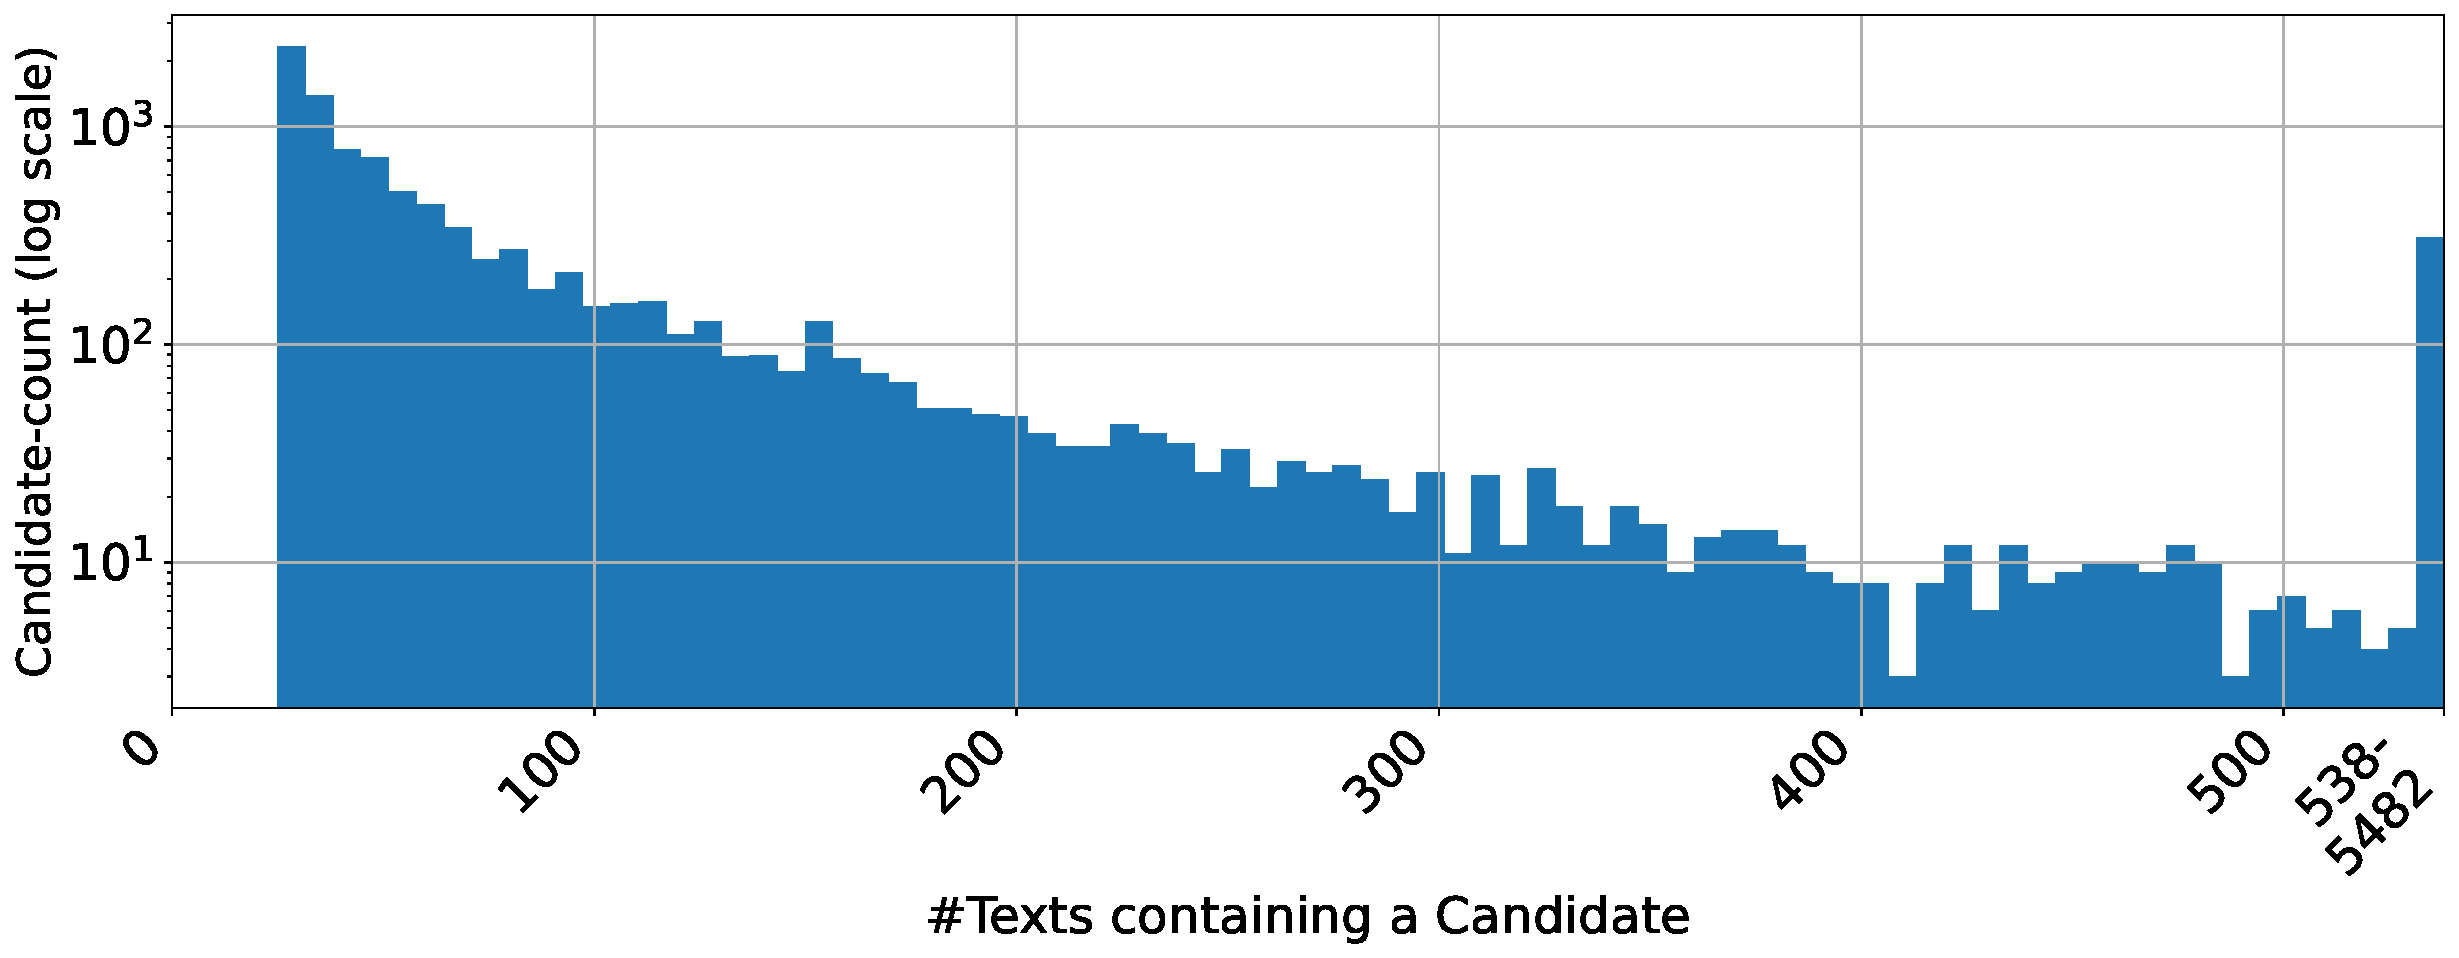
\includegraphics[width=\figwidth]{graphics/dataset_new/docs_per_phrase.pdf}
	\caption[Distribution of texts per candidate]{Distribution of texts per candidate (log scale), cut off at the 97\textsuperscript{th} percentile. \Gls{df}-threshold for a candidate is set to 25, yielding 10\,060 candidates for 11\,601 documents. Median number of documents per candidate is 49 and for the 95\textsuperscript{th} percentile 375. 2595 candidates occur in at least 100 descriptions.}
	% Occurences in all Documents per Keyphrase (for all keyphrases that occur $\geq$ 5 times, cut off at the 93th percentile). 7007 of 45295 terms occur at least 5 times. Most frequent phrases: seminar (4173), course (3722), students (2923), it (2671), language (2071), work (1980), event (1842), research (1731), lecture (1723), law (1719).
	\label{fig:candidate_histogram}
\end{figure}

These results show that the algorithm produces much less candidates for our dataset compared with the originally considered ones. Because of that, the subsequent steps of the algorithm have a less rich representation to choose from, decreasing the chance to achieve good performances downstream.

\section{Results for the Siddata-dataset}
\label{sec:results_siddata}

\todoparagraph{The plots here show the results from several different parameter-configurations. Because of that, the extracted semantic directions and also the metrics may differ between the plots. This is not a bug but a feature - they are all differnent but all are nice}

As previously described, the primary method used here to check if the described methodology works for the domain of educational resources is to check if low-depth decision trees trained on the extracted semantic directions of the Siddata-dataset can classify a courses' faculty. Before doing that however, it is important to first validate if it can reasonably assumed that the faculty \textit{can generally} be extracted from only the descriptions associated with the entities.

\subsection*{Extracing faculties without the algorithm}

\begin{figure}[h]
	\begin{center}
	  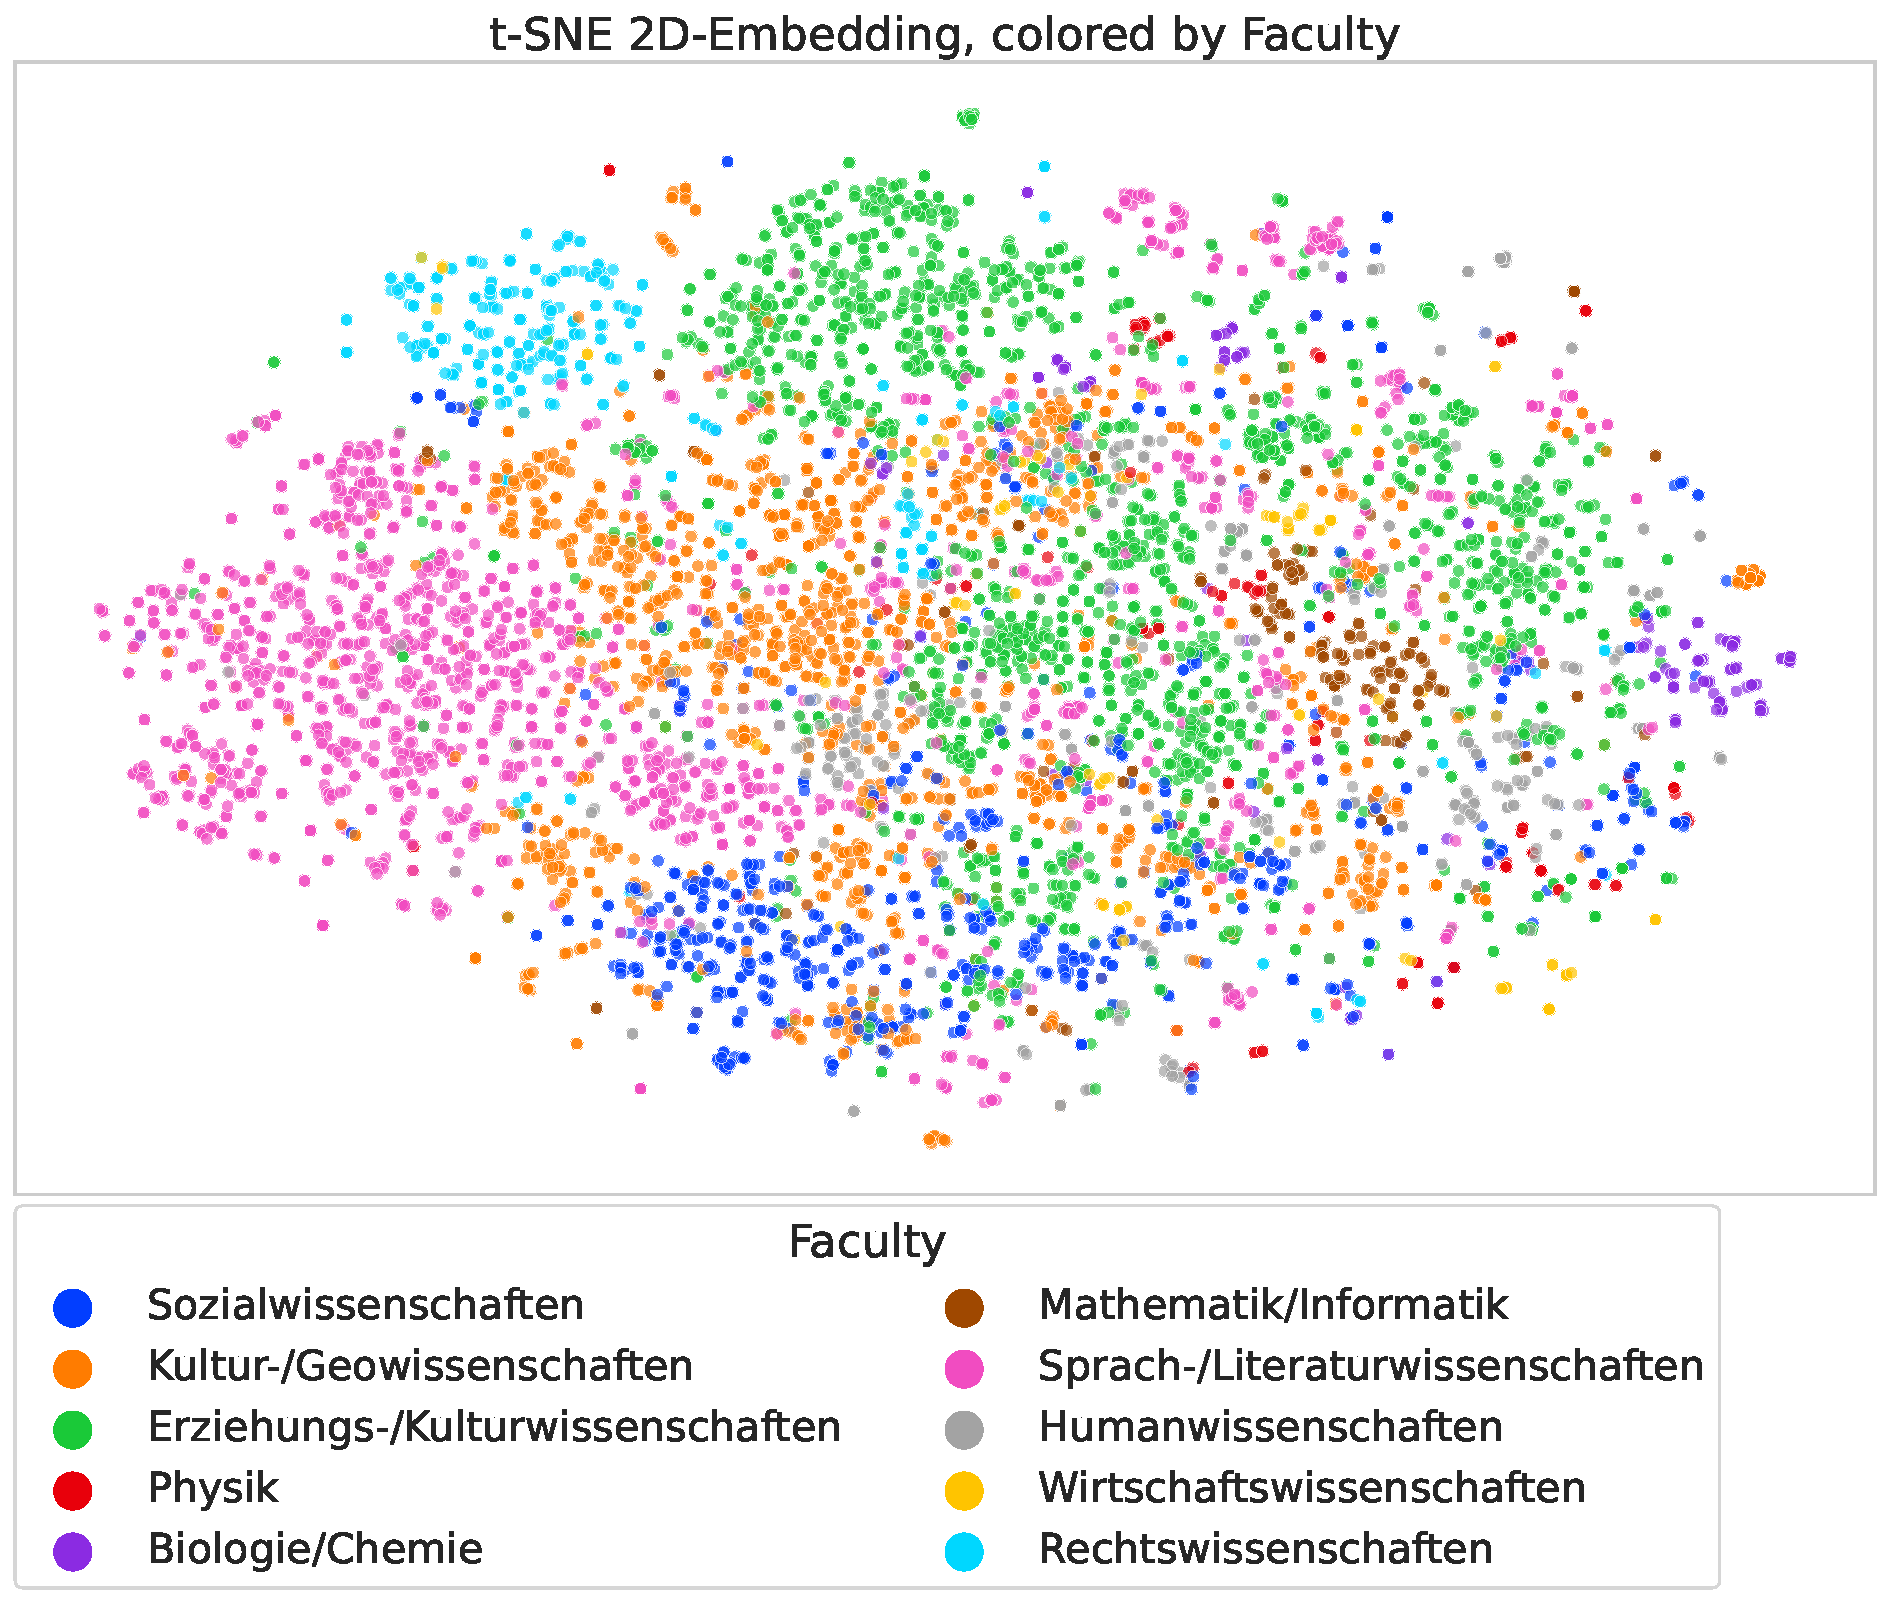
\includegraphics[width=0.9\textwidth]{graphics/dataset_new/scatter_mds_tsne_e2a70a9bf2.pdf}
	  \slcaption{2D Visualization of the Course-dissimilarity matrix, generated with \gls{tsne}. See \url{https://github.com/cstenkamp/derive_conceptualspaces/blob/main/notebooks/text_referenced_plots/visualize_embeddings.ipynb} for the origin of this plot as well as a 3D-plot on unaltered 3D-MDS-data that doesn't rely on t-SNE.}
	  \label{fig:scatter_mds_siddata}
	  % möchte sagen: Die Embeddings Clustern -> es lassen sich "sinnvolle Sachen" (wie faculty) draus ziehen.
	\end{center}
\end{figure}

To see if it is possible to extract any kind of structured data from the unstructured course descriptions, a \gls{bert}-based Neural Network classifier was trained on the dataset, classifying the subset of courses that are for the \gls{uos} to the faculty they belong to. The architecture of the classifier is described in the Appendix~\ref{sec:faculty_classifier}

The classifier trained for 12 epochs before \emph{stopping early} due to its performance on the test-set decreasing. It achieved an accuracy of \textbf{85.19\%} for the test-set (94.13\% on the training set), providing strong indication that the faculty can be considered a latent property of its description. Because \gls{bert} is one of the best general language classifiers to date \cite{Devlin2019}, this accuracy will be considered the upper boundary for the results of our algorithm.

\autoref{fig:scatter_mds_siddata} displays a \gls{tsne}-representation of the dissimilarity matrix generated from the normalized angular distances (\autoref{eq:norm_ang_dist}) of the \gls{bow}-representations generated from the courses (only those from the \gls{uos}) A first comparison of this scatter-plot and its placetypes-counterpart (\autoref{fig:scatter_mds_placetypes}) reveals that Siddata appears to have more homogenous clusters.

From this distance matrix, the algorithm subsequently creates an embedding using the \gls{mds}-algorithm to afterwards train multiple \glspl{svm} for each of the extracted candidate-dimensions before re-embedding the entities into a new space where the dimensions encode the \gls{rank} for each of the extracted features. To evaluate the algorithm, we will check if it is to be able to classify the faculty with a decision tree that uses between one and maximally $2^3=8$ of these features. To provide a context for the resulting performance, we will first look at a classification which does not use the feature-based representation, but on a raw low-dimensional embedding without class-specific dimensions. This can be seen as the lower boundary of what a classification without selecting the most relevant dimensions but instead use an optimal but general three-dimensional space can achieve. A classification-performance of low-level decision trees that use only the most important features from all available ones that is higher than this thus provides evidence that the detected features encode important distinctive properties. \autoref{fig:mds_3d_hyperplane} visually represents the result of the classification using a linear \gls{svm} on a three-dimensional space generated as result of \gls{mds} on the dissimilarity matrix of the entities. Averaged over all Faculties, this classifier reaches a weighted accuracy of 64.3\% (unweighted accuracy 69.0\%, weighted F1: 0.414, unweighted F1: 0.269). Note that these values are reached by training on the full data without a separate testing-set.
% text_referenced_plots/siddata_analysis/visualize_embeddings_mds.ipynb


\begin{figure}[h]
	\begin{center}
	  \makebox[\textwidth][c]{
		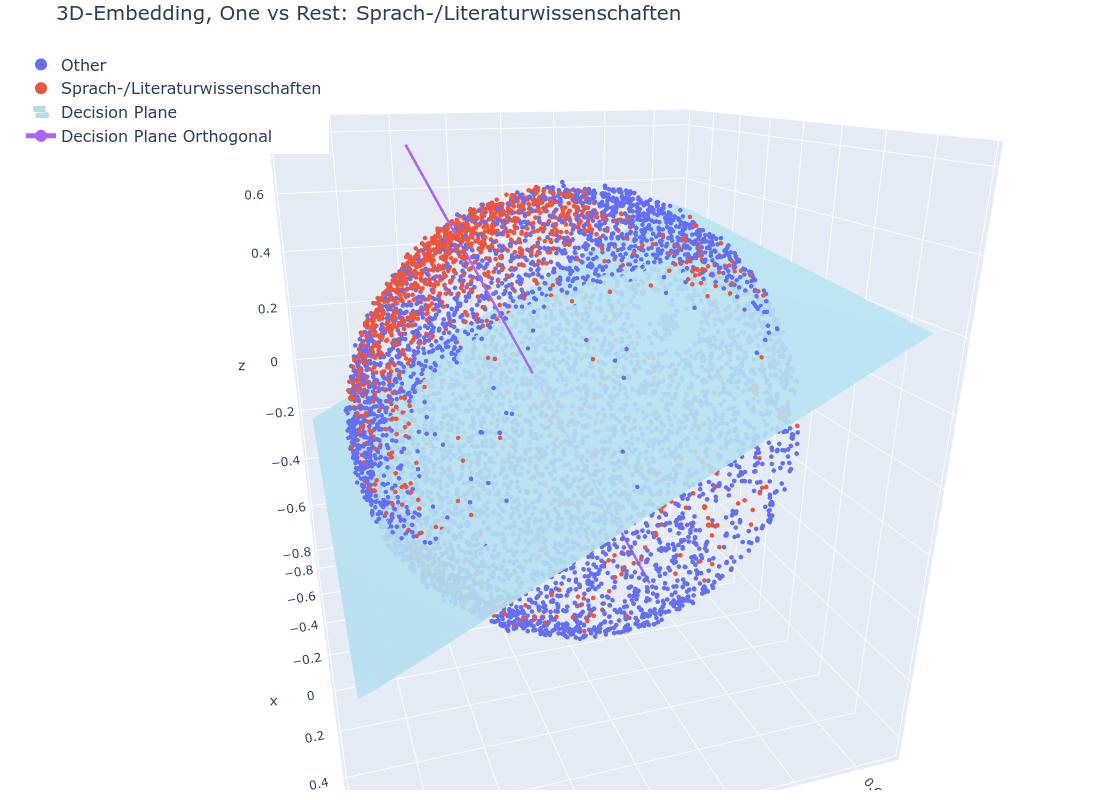
\includegraphics[width=1.1\textwidth]{graphics/dataset_new/possibledecision_sprachlit.png}
		\slcaption{A possible Hyperplane on a 3-Dimensional Embedding. The SVM depicted here reaches an Accuracy of 67.9\% (Precision: 39.8\%, Recall: 70.5\%). Visualize interactively: \url{https://github.com/cstenkamp/derive_conceptualspaces/blob/main/notebooks/text_referenced_plots/visualize_embeddings_mds.ipynb} }
		\label{fig:mds_3d_hyperplane}
		%möchte sagen: To say what the lower boundary of what a 3D-Embedding of NON-CLASS-SPECIFIC dimensions can yield for classification, 
		% wie related der space von fig:boxes_rechtswis mit den interpretable dimensions zu IRGENDEINEM 3D-Space
	  }
	\end{center}
\end{figure}


\subsection*{Extracing faculties with \glspl{dt} based on the algorithm}

Now that we have established upper and lower boundary for what can reasonably be expected from the algorithm, let us finally look at the performance of its decision-trees, to gain evidence if human concepts are encoded in its extracted features. \autoref{tab:robustresults_perfb} lists average accuracies per faculty for decision trees created on the basis of a single hyperparameter-configuration that was selected to achive high performance on average. The respective values are the average and standard-deviation of runs with 5-fold crossvalidation each for trees of various depths. The results show high accuracies across all faculties even for low-depth trees, but the faculty \textit{Humanwissenschaften} displays a high standard deviation for that condition.

\begin{table}[H]
	\resizebox{\textwidth}{!}{%
		\begin{tabular}{rcccc}
		\toprule
		\textbf{Depth} & \textbf{1} & \textbf{2} & \textbf{3} & \textbf{unbound} \\
		\midrule
		\textbf{Sozialwissenschaften} & 0.831 ± 0.021 & 0.811 ± 0.033 & 0.780 ± 0.028 & 0.918 ± 0.006 \\
		\textbf{Kultur-/Geowissenschaften} & 0.806 ± 0.010 & 0.728 ± 0.066 & 0.813 ± 0.022 & 0.873 ± 0.008 \\
		\textbf{Erziehungs-/Kulturwissenschaften} & 0.791 ± 0.010 & 0.824 ± 0.010 & 0.828 ± 0.020 & 0.868 ± 0.008 \\
		\textbf{Physik} & 0.747 ± 0.054 & 0.770 ± 0.033 & 0.818 ± 0.038 & 0.983 ± 0.003 \\
		\textbf{Biologie/Chemie} & 0.787 ± 0.044 & 0.838 ± 0.049 & 0.890 ± 0.036 & 0.982 ± 0.004 \\
		\textbf{Mathematik/Informatik} & 0.866 ± 0.031 & 0.844 ± 0.051 & 0.882 ± 0.038 & 0.978 ± 0.004 \\
		\textbf{Sprach-/Literaturwissenschaften} & 0.832 ± 0.009 & 0.832 ± 0.009 & 0.862 ± 0.009 & 0.902 ± 0.008 \\
		\textbf{Humanwissenschaften} & 0.630 ± 0.130 & 0.768 ± 0.103 & 0.781 ± 0.093 & 0.949 ± 0.005 \\
		\textbf{Wirtschaftswissenschaften} & 0.903 ± 0.015 & 0.910 ± 0.034 & 0.924 ± 0.018 & 0.989 ± 0.003 \\
		\textbf{Rechtswissenschaften} & 0.948 ± 0.031 & 0.894 ± 0.015 & 0.952 ± 0.011 & 0.985 ± 0.003 \\
		\textbf{Mean (weighted)} & 0.814 ± 0.035 & 0.822 ± 0.040 & 0.853 ± 0.031 & 0.943 ± 0.005 \\
		\textbf{Mean (unweighted)} & 0.810 ± 0.020 & 0.806 ± 0.031 & 0.835 ± 0.023 & 0.901 ± 0.007 \\
		\bottomrule
		\end{tabular}
	}
	\slcaption{Robust cccuracies per faculty of a well-performing configuration. The reported results are mean and standard deviation from the result of ten runs with 5-fold crossvalidation each.\hideref{tab:robustresults_perfb_f1}{F1-Table}}
	\label{tab:robustresults_perfb}
\end{table}

Keep in mind that accuracies often makes the situation look better than it is. The weighted average F1-scores are between 0.505 (depth 1) and 0.710 (unbounded). For the full table of F1-scores it is referred to the appendix, specifically \autoref{tab:robustresults_perfb_f1}. 

Compared with the results of the \gls{bert}-based classifier (85.19\%), the achieved results are suprisingly competative, with the weighted mean of trees of depth one and two only slighly below that, and deeper trees achieving even higher accuracies. 
% "suprisingly competative" ersetzen mit "soundso ist der przentsatz, soundso ist unserer, wir observen soundsoeinen unterschied"
\todoparagraph{We said in the previous section that there are less candidates, making it harder. These quantifiable results show that it appears to work anyway}  % "wie in 4.2 gibts weniger candidates, was es downstream schwieriger macht, aber wie in 4.3 klappts ja trotzdem." => Das geht selbst in results, da es eine quantifizierbare darstellung von verhältnismäßigkeiten ist und keine bewertung
Importantly however, the results reported here are those of a sepearate classifier per faculty (1-vs-rest), differentiating only between the respective faculty as positive class and all other faculties as negative class. As will be further elaborated in the discussion, this is the only realistic way of doing it: A binary tree of depth one can differentiate between maximally two classes and thus maximally achieve a classification by perfectly classifying the most frequent class and labelling all samples as the second most frequent class, which in the case of faculties is $(2011+1665)/7081=51.9\%$. Results for such trees are reported in \autoref{tab:robustresults_allatonce}.

\begin{table}[H]
	\begin{tabular}{rccccc}
		\toprule
		\textbf{Depth} &  \textbf{1} & \textbf{2} & \textbf{3} & \textbf{any} \\
		\midrule
		\textbf{Accuracy} & 0.056 ± 0.008 & 0.078 ± 0.042 & 0.196 ± 0.017 & 0.584 ± 0.015 \\
		\textbf{F1}       & 0.072 ± 0.006 & 0.125 ± 0.014 & 0.199 ± 0.007 & 0.513 ± 0.020 \\
		\bottomrule
	\end{tabular}
	\caption[Robust scores for classifying all faculties at once]{Robust scores of a well-performing configuration for classifying all faculties at once. The reported results are mean and standard deviation from the result of ten runs with 5-fold crossvalidation each.}
	\label{tab:robustresults_allatonce}
\end{table}


\subsubsection{Recovering entities from salient directions}
\label{sec:duplicate_maps}

After having tested if our semantic embedding captures at least one prominent latent topic of the data, we will additionally check if the produced embedding adequately captures enough of the general variability of the data. For that, we check if it is possible to recover entities from the salient directions, to ensure that no important relevant information was lost when mapping them to their semantic embedding. To get a general understanding, let us consider under what circumstances multiple different entities will fall towards the exact same coordinates. 

To get an estimate of the importance of each dimension of the embedding, we started with a full matrix where each entity is defined via each semantic direction. Starting with a 200-dimensional space, we removed random directions. Further we applied different levels of discretisation to the remaining dimensions. We are wondering what amounts of discretisation and removal of dimensions is necessary for multiple entities to fall onto the same category. Each combination was done multiple times, each time removing other random directions, and the percentage of duplicates in the data was counted. \autoref{tab:duplicates_per_comb} displays the result of this.

\begin{table}
	\caption[Duplicates per combination of dimensionality and discretisation-categories]{Duplicates per combination of dimensionality and amount of categories per left-over category. Row = number of left-over dimensions, cols = discretisation (number in parantheses is the divisor of the orginal value)}
	\begin{tabular}{lrrrrrr}
	\toprule
	 & \textbf{2} & \textbf{11} & \textbf{23} & \textbf{116} & \textbf{232} & \textbf{1160} \\
	\#dims & (5800) & (100) & (50) & (10) & (5) & (2) \\
	\midrule
	3 & 100\% & 99.85\% & 68.98\% & 6.85\% & 5.25\% & 3.97\% \\
	5 & 100\% & 24.91\% & 9.79\% & 5.25\% & 4.72\% & 3.42\% \\
	10 & 100\% & 10.18\% & 6.90\% & 4.67\% & 4.23\% & 2.11\% \\
	20 & 100\% & 7.41\% & 5.58\% & 4.23\% & 3.52\% & 0.79\% \\
	50 & 99.97\% & 5.46\% & 4.72\% & 3.19\% & 1.89\% & 0.05\% \\
	100 & 99.88\% & 4.80\% & 4.18\% & 1.94\% & 0.65\% & 0\% \\
	200 & 99.55\% & 4.36\% & 3.44\% & 0.67\% & 0.09\% & 0\% \\
	\bottomrule
	\end{tabular}
	\label{tab:duplicates_per_comb}
\end{table}




\subsection{Qualitative Analysis}

The main goal of the algorithm is not to optimally classify the respective faculties optimally, but to find semantic directions. Thus, once it has been established that the performance is reasonably well, looking at the names of these directions is just as important. \autoref{fig:dims_for_fb} visually represents decision-trees for each of the faculties of depth one, \ie trees that can only use a single semantic direction for their decision. With the exception of the faculties \emph{Physik} and \emph{Biologie/Chemie}, the semantic directions that best predict each faculty appear very relevant to the respective topic.

\begin{figure}[h]
	\begin{center}
	  \makebox[\textwidth][c]{
		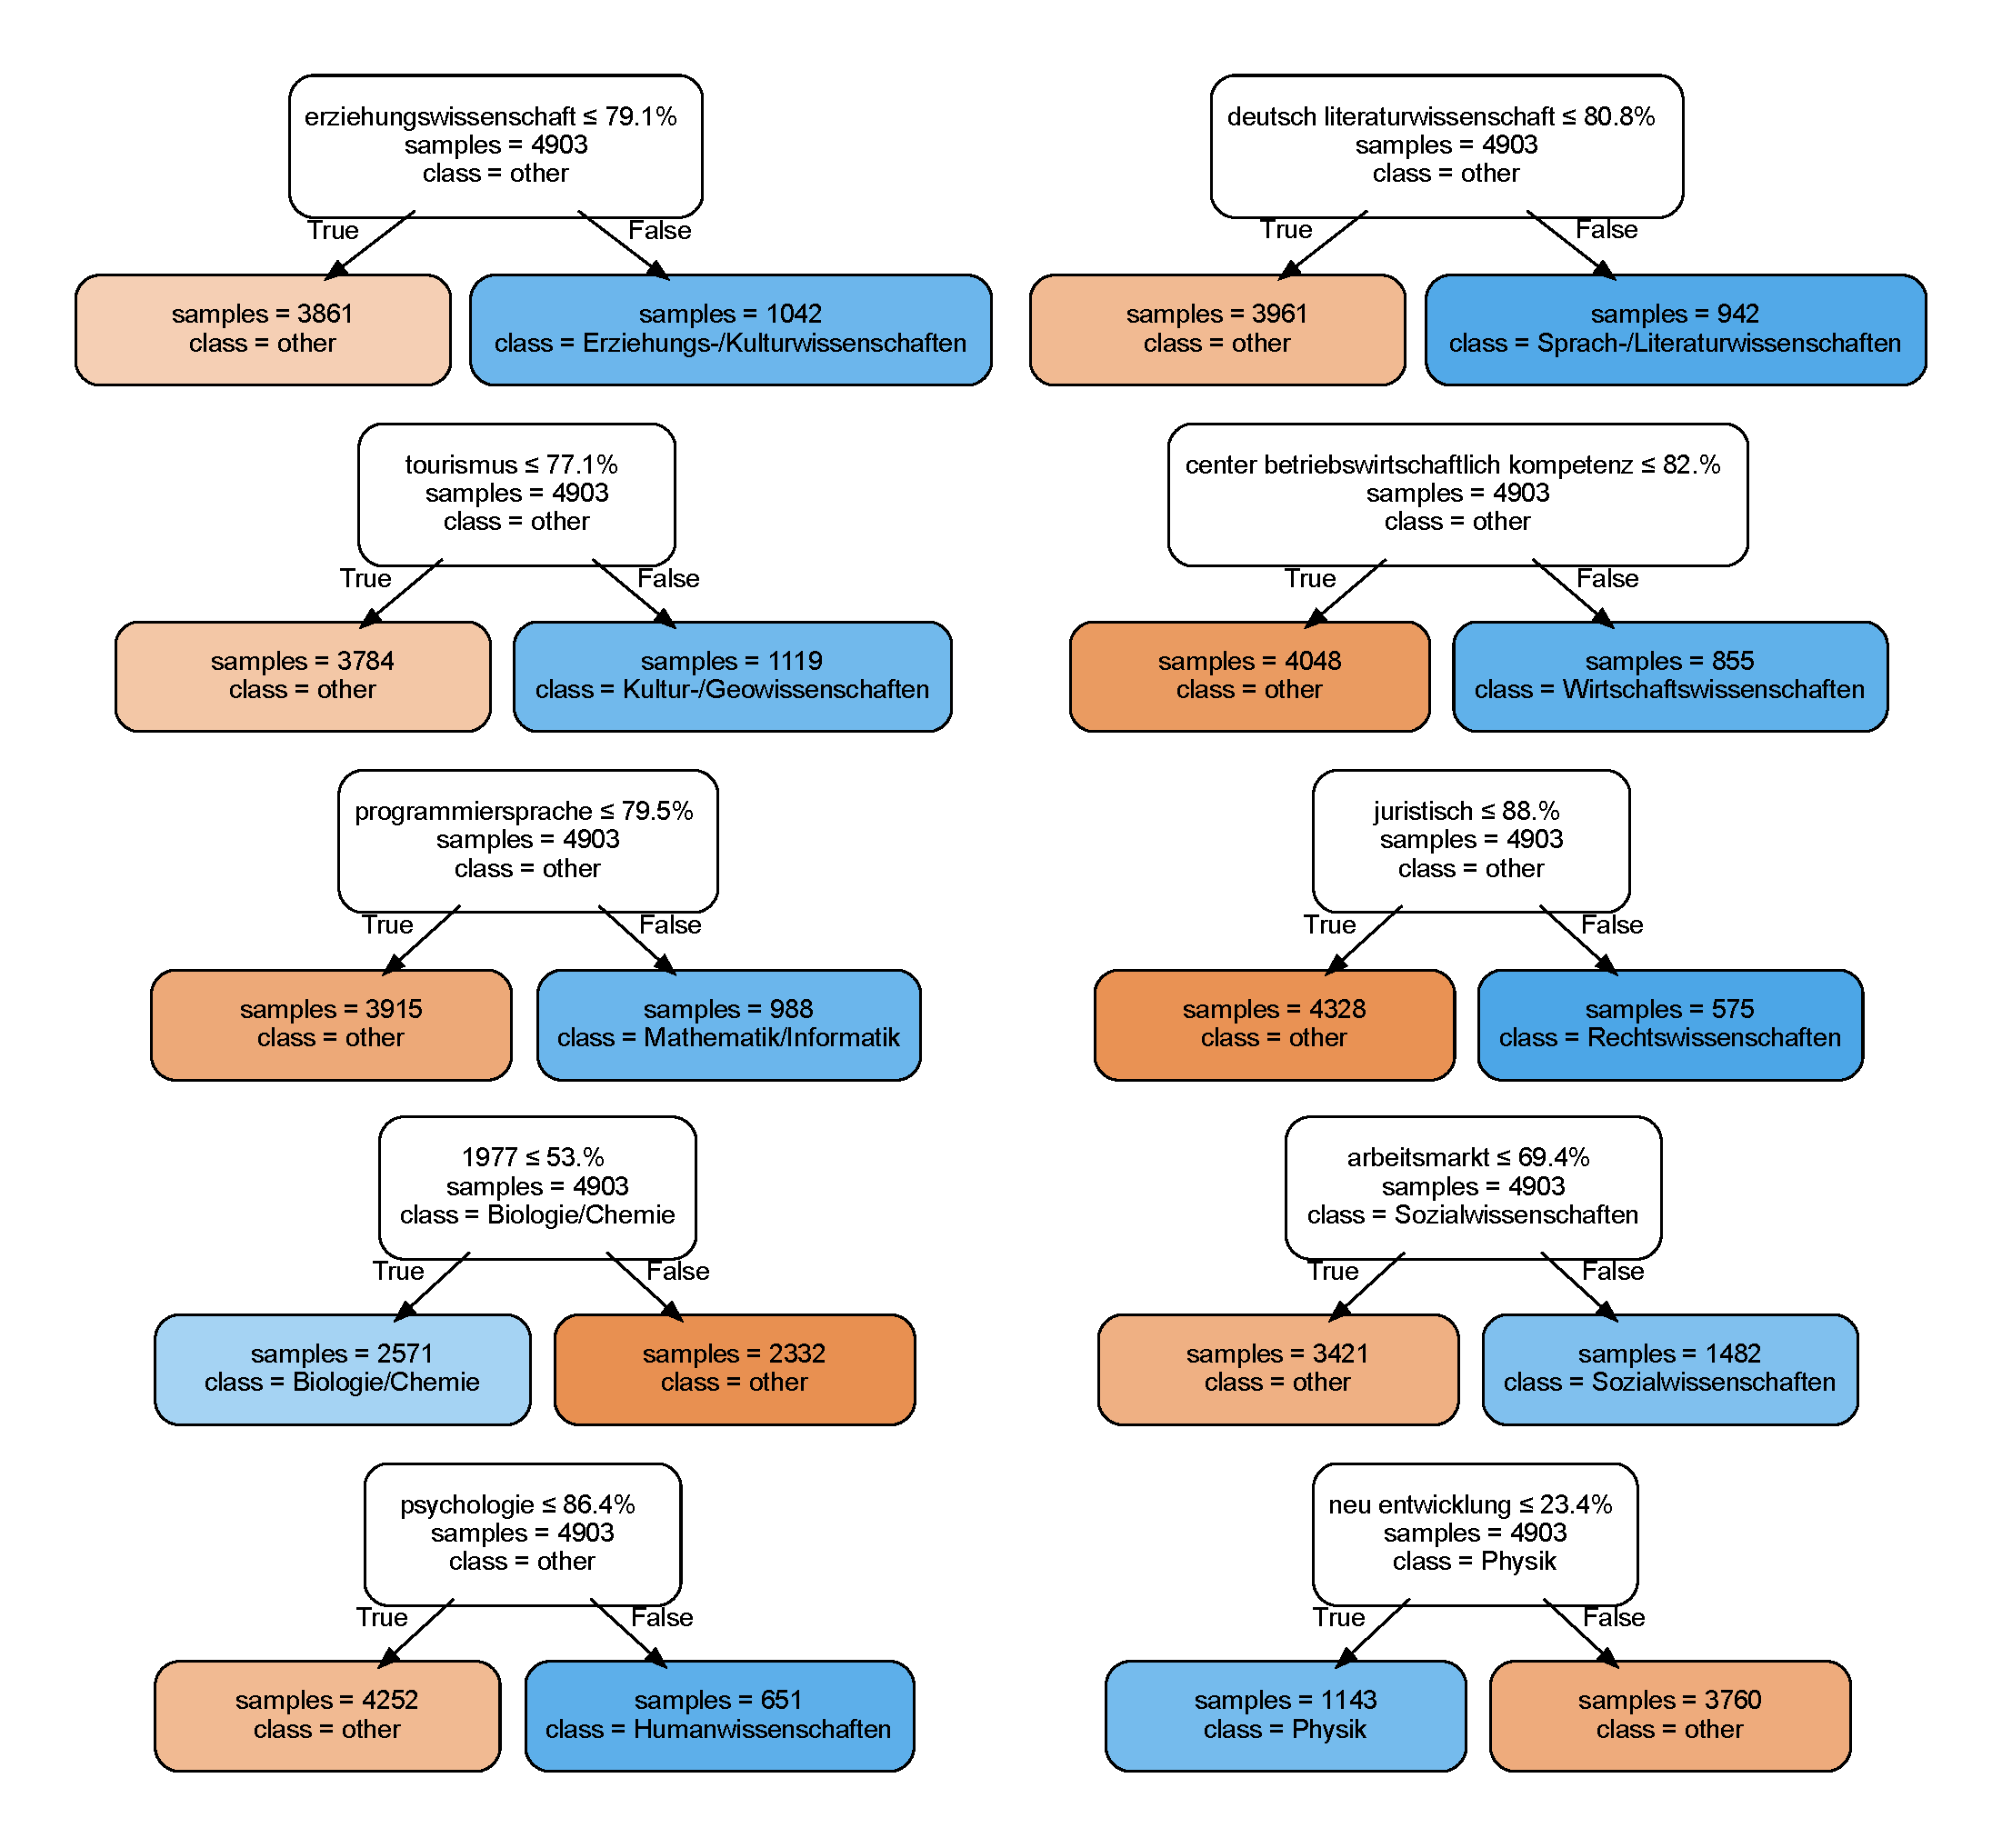
\includegraphics[width=1.3\textwidth]{graphics/dataset_new/dims_for_fb.pdf}
		\slcaption{Resulting \glspl{dt} with only a single decision for each of the faculties. The white boxes show a semantic direction and the maximal rank \wrt to this direction for an entity to fall under the class designated by the respective left branch.}
		\label{fig:dims_for_fb}
		% möchte sagen: Unsere Extracted Dimensions entsprehcen human concepts wie Fachbereich
	  }
	\end{center}
\end{figure}

For trees deeper than one level, the selected features from the second level on are not necessarily the most important ones.\footnote{A \gls{dt} has separate conditions for every subtree, which means on level two there are two different features that depend on the result of the first split} Instead it is possible to extract the most important features for a classification by looking at the respective information gain achieved by splitting it. \autoref{tab:courses_top3} displays the resulting three most important directions for each of the respective faculties. While the details of this result will be eloborated upon in the discussion, most of the detected features appear convincing. \todoparagraph{remove sentence} Regarding an actual classification using these features, \autoref{fig:boxes_rechtswis} in the Appendix displays the result of a sample classification of a decision tree with three features.


\begin{table}[H]
	\makebox[\textwidth][c]{
		\resizebox{1.1\textwidth}{!}{%
		\setlength{\tabcolsep}{2pt}
		\begin{tabular}{r@{\hskip 8pt}lllcr@{\hskip 6pt}c}
		& & & & \multicolumn{2}{c}{\textbf{Accuracy}} \\
		\textbf{Faculty} & \multicolumn{3}{c}{\textbf{Top 3 Directions}} & \textbf{Top 3} & \textbf{Top 1} \\
		\midrule
		\textbf{Erziehungs-/Kulturw.} & erziehungswissenschaft & okumenisch & english for & 78.02\% & 75.50\% \\
		\textbf{Rechtswissenschaften} & juristisch & bgb & bgb & 95.86\% & 91.10\% \\
		\textbf{Wirtschaftsw.} & {\scriptsize center betriebswirtschaftlich kompetenz } & religionsunterrichts & design & 89.65\% & 79.10\% \\
		\textbf{Kultur-/Geow.} & tourismus & gi & stadtgeographie & 75.50\% & 77.44\% \\
		\textbf{Mathem./Informatik} & programmiersprache & menge & hoffnung & 93.00\% & 91.85\% \\
		\textbf{Sprach-/Literaturw.} & deutsch literaturwissenschaft & sprache & okumenisch & 86.71\% & 85.10\% \\
		\textbf{Humanwissenschaften} & psychologie & metaphysik & internationalisierung & 86.84\% & 85.51\% \\
		\textbf{Physik} & neu entwicklung & mitarbeiterinnen & {\small regelmassig aktiv teilnahme} & 78.27\% & 77.36\% \\
		\textbf{Biologie/Chemie} & aktivierung studierend & brd & berucksichtigung finden & 85.22\% & 62.13\% \\
		\textbf{Sozialwissenschaften} & arbeitsmarkt & regieren & multiple & 78.60\% & 67.63\% \\
		\end{tabular}
		\slcaption{Top 3 directions to detect the respective faculty from the data. Note that it may also be the case that low values for the respective feature encode class membership.}
		\label{tab:courses_top3}
		}
	}
\end{table}


\newcolumntype{L}[1]{>{\raggedright\let\newline\\\arraybackslash\hspace{0pt}}m{#1}}
\newcolumntype{C}[1]{>{\centering\let\newline\\\arraybackslash\hspace{0pt}}m{#1}}
\newcolumntype{R}[1]{>{\raggedleft\let\newline\\\arraybackslash\hspace{0pt}}m{#1}}



\begin{table}[h]
	\centering
	\makebox[\textwidth][c]{
		\resizebox{1.1\textwidth}{!}{%
	\begin{tabular}{R{0.2\textwidth}|L{0.9\textwidth}}
	   Cluster Center & Cluster Elements \\ \midrule
				 opnv & befragungen, bewohner, urbanen, 00 uhr \\
	   bertolt brecht & brecht, exil, bertolt, weiss, weimarer republik, auschwitz, weimarer, ... \\
religionswissenschaft & religionsunterrichts, spirituelle, religions, teil veranstaltung, religion, studienbeginn, auml ischen, ... \\ 
		 erkrankungen & klinischen, gesundheitlichen, krankheit, rehabilitation, pravention, aufrechterhaltung, exemplarische inhalte, ... \\
	  		  lineare & integrierte, berechnung, variablen, skript, ubungsaufgaben, losung, vorliegen \\
	 		 parteien & verfassung, demokratischen, zivilgesellschaft, semester sowie, einander, folgendem link, sozialwiss uni osnabrueck, ... \\
	 		 kleidung & textilien, mode, textile, parallelen \\
			    kreuz & heilige, christentum, 1957, fuhrungen \\
 		 offentliches & offentlichkeitsarbeit, verwaltungsrecht, offentlichen recht, offentliches recht, europarecht, staatsrecht, teilnahmevoraussetzungen veranstaltung, ... \\
	    masterstudium & fortgeschrittene, schlusselkompetenzen, betriebswirtschaftslehre, untereinander \\
	unterrichtspraxis & fachlichen, unterrichtsplanung, schulalltag, lehrerinnen, schulische, daz, bildung nachhaltige, ... \\
  		  aristoteles & asthetik, semantik, dialoge, menschheit, sucht, benutzt, philosophische, ... \\
   		   mythologie & athen, mythos, mann, griechen, ubersetzung, figur, griechischen, ... \\
 		 flexibilitat & weiterbildung, schlusselqualifikation, erfolgreiches, fordert, vorlagen, strukturierte, berufsleben, ... \\
   aktive beteiligung & teilnahme ersten, wochentliche, zweit, festlegung, ubergreifende, auml ndige, ndige, ... \\
 		 unsicherheit & covid 19 pandemie, korperlich, wendet studierende, webinar, risiko, einbringen, fachlich, ... \\
	 wirtschaftlicher & industrialisierung, wachstum, republik, wirtschaftspolitik, konkurrenz, positive, russland, ... \\
	\end{tabular}
	}}
	\label{tab:clusters}
	\caption{Exemplary clusters found in the Siddata-dataset}
\end{table}	


% \removeMe{
% \subsubsection{Are the phrases making up the semantic-direction-clusters similar?}
% \todo
% \subsubsection{Are there dimensions encoding the COVID-19 pandemic?}
% \todo
% \subsubsection{Is there a direction capturing advanced courses?}
% \todo
% }



% \subsubsection{Extended analysis}
% \removeMe{
% \todoparagraph{Also interesting: The top-ranked entities for some of the features }

% \todoparagraph{Neben den Clustern die ich mir anzeigen lassen kann und qualitativ analysieren kann}, kann ich mir auch die distances to the origins of the respective dimensions (induced by the clusters), what induces the respective rankings! (see DESC15 p.24u, proj2 of load_semanticspaces.load_projections) anzeigen lassen - da kann ich sagen "term xyz ist bei "nature" am höchsten".
% }




\origsection{Optimal Parameters}
\label{sec:results_params}

Having established the algorithm's ability to be transferred to the domain of educational resources, we will conclude this chapter with the results of our hyperparameter search. The algorithm was run with hundreds of different hyperparameter-combinations for both the placetypes- and Siddata-dataset throughout the process of its implementation and testing. As the precise hyperparameter-combination was not very imporant for our research questions, only some exemplary results for the Siddata-dataset will be reported here for the sake of brevity.

The reports produced in the previous section are the best ones from a final set of 165 different parameter-combinations, run over the course of three days on the \gls{ikw}-grid. \todoparagraph{which was in contrast to the mainalgos easy thanks to my scalable implementation hehe} 


Generally, we selected a parameter-configuration that reached a high accuracy on average for the aforementioned classifiation based on shallow decision trees as representatively \textit{good} configuration. Here we compare all of the parameter-combinations that were considered - however the printed tables are shortened for a clearer overview.

As described in \autoref{sec:svm_filter_cands}, a good first approximation for the quality of an embedding is to check how many candidate-terms get a kappa-score which is above the threshold of $0.5$. Unfortunately, \cite{Derrac2015} and its follow-ups \cite{Ager2018,Alshaikh2020} did not explictly and unambiguously state how the kappa-score was calculated. Not only does its implementation\footnote{\todoparagraph{Link}} have many arguments, but also the application may vary. In general, it compares the \textit{prototypicality} according to the classificiation decision with the \gls{quant} of how often the according word occurs in the entities' associated texts. The precise mechanism of has however many more parameters: for example, one can only consider those entities that have a positive \gls{quant}-score, such that not almost all of the candidates have a score of zero\footnote{For the movies-dataset, a \gls{df} threshold of 100 for a candidate means that up to 14\,900 entities (99.33\%) do not contain the entities, meaning all scores and accordingly also their rank will be zero. In constrast to that, the ranking induced by mapping of the high-dimensional and real-valued embeddings onto the separatrix orthogonal will almost always lead to unique ranks.}. Another open question is when considering the raw count as quantification\footnote{The exact wording of \textcite{Derrac2015} is: \textit{\q{[...] measure the correlation between the ranking induced by \vec{v_t} and the number of times t appears in the documents associated with each entity [...]}}. This seems to imply that they are using the raw count, even though \cite{Ager2018,Alshaikh2020} write in their algorithm summary that they used the \gls{ppmi}-score}, if the rankings induced by the orthogonal of the hyperplane are to be compared with the raw count, or the \textit{ranking induced} by the count. To clarify this ambiguity, we tried out many different interpretations for this score. 

\autoref{tab:kappa_table} (moved to the Appendix) shows the results of many runs with different parameter-combinations with the purpose of figuring out which combination of parameters and kappa-metrics lead to enough candidate-terms. The meaning of the different kappa-scores encoded in the columns is given in the implementation details in \autoref{tab:kappa_measures}. \todoparagraph{Also ref the figure of workflow where we check what threshold was realistic}. The table shows drastically differing values for the individual scoring methods. To understand if the difference in scoring has an effect on \textit{which} candidates are extracted, let us look at the overlap of different measures in \autoref{tab:kappa_overlap}. \todoparagraph{Zeigt er hier ?? ?}


\begin{table}[H] 
	\resizebox{\textwidth}{!}{%
	\begin{tabular}{rccccccccccccc}
		\toprule
		 & \textbf{accuracy} & \textbf{precision} & \textbf{recall} &  \textbf{f1} & \textbf{r2r-d} & \textbf{r2r-min} & \textbf{b2b} & \textbf{dig} & \textbf{c2r+} & \textbf{r2r+d} & \textbf{r2r+min} & \textbf{r2r+max} & \textbf{dig+2} \\
		 & (10060) & (1668) & (10060) & (3155) & (0) & (2) & (3052) &  (0) & (4) & (0) & (239) & (103) & (1010) \\
		\midrule
		accuracy & - & 0.166 & \bfseries 1.000 & 0.314 & 0.000 & 0.000 & 0.303 & 0.000 & 0.000 & 0.000 & 0.024 & 0.010 & 0.100 \\
		precision & \bfseries 1.000 & - & \bfseries 1.000 & \bfseries 1.000 & 0.000 & 0.001 & 0.998 & 0.000 & 0.002 & 0.000 & 0.084 & 0.051 & 0.126 \\
		recall  & \bfseries 1.000 & 0.166 & - & 0.314 & 0.000 & 0.000 & 0.303 & 0.000 & 0.000 & 0.000 & 0.024 & 0.010 & 0.100 \\
		f1  & \bfseries 1.000 & 0.529 & \bfseries 1.000 & - & 0.000 & 0.001 & 0.967 & 0.000 & 0.001 & 0.000 & 0.067 & 0.032 & 0.140 \\
		r2r-d  & 0.000 & 0.000 & 0.000 & 0.000 & - & 0.000 & 0.000 & 0.000 & 0.000 & 0.000 & 0.000 & 0.000 & 0.000 \\
		r2r-min  & \bfseries 1.000 & \bfseries 1.000 & \bfseries 1.000 &  \bfseries 1.000 & 0.000 & - & \bfseries 1.000 & 0.000 & 0.000 & 0.000 & 0.000 & 0.000 & 0.000 \\
		b2b  & \bfseries 1.000 & 0.546 & \bfseries 1.000 & \bfseries 1.000 & 0.000 & 0.001 & - & 0.000 & 0.001 & 0.000 & 0.068 & 0.033 & 0.141 \\
		dig & 0.000 & 0.000 & 0.000 & 0.000 & 0.000 & 0.000 & 0.000 & - & 0.000 & 0.000 & 0.000 & 0.000 & 0.000 \\
		c2r+  & \bfseries 1.000 & \bfseries 1.000 & \bfseries 1.000 & \bfseries 1.000 & 0.000 & 0.000 & \bfseries 1.000 & 0.000 & - & 0.000 & \bfseries 1.000 & \bfseries 1.000 & 0.250 \\
		r2r+d  & 0.000 & 0.000 & 0.000 & 0.000 & 0.000 & 0.000 & 0.000 & 0.000 & 0.000 & - & 0.000 & 0.000 & 0.000 \\
		r2r+min  & \bfseries 1.000 & 0.586 & \bfseries 1.000 & 0.887 & 0.000 & 0.000 & 0.874 & 0.000 & 0.017 & 0.000 & - & 0.406 & 0.452 \\
		r2r+max  & \bfseries 1.000 & 0.825 & \bfseries 1.000 & 0.981 & 0.000 & 0.000 & 0.981 & 0.000 & 0.039 & 0.000 & 0.942 & - & 0.437 \\
		dig+2  & \bfseries 1.000 & 0.208 & \bfseries 1.000 & 0.438 & 0.000 & 0.000 & 0.426 & 0.000 & 0.001 & 0.000 & 0.107 & 0.045 & - \\
		\bottomrule
	\end{tabular}
	\slcaption{Overlap of different scoring methods in percent. Numbers in parantheses list the total number of extracted samples for each scoring method. Upper right triangle encodes the cardinality of the union divided by the cardinality of column-method, lower left triangle divides by row.}
	\label{tab:kappa_overlap}
	}
\end{table}
	
This table additionally reports the raw \textit{accuracy, precision, recall} and \textit{f1}-scores of the classifier. The overlaps of these scores will  serve to test our hypothesis that due to the different nature of the Siddata-dataset, comparing the \textit{ranking} of the candidates leads to worse performances than comparing raw classification scores (also suggested by \cite{Ager2018}).

After these preliminary analyses with the number of extracted candidates, let us also quickly look at differences in perforamances of the decision-trees depending on parameter-combinations. \autoref{tab:best_params} lists the accuracies of \glspl{dt} classifying a course's faculty per parameter-setup for some of the configurations of the final run. Specifically, this compares accuracies for several \textit{1vsRest} decision trees of depth one with a test-set size of 33\%.


\newcommand{\SmfauhcsdT}{\setlength\extrarowheight{-5pt} \scriptsize \mfauhcsdT}
\newcommand{\Smfauhtcsldp}{\setlength\extrarowheight{-5pt} \scriptsize \mfauhtcsldp}

% Other configs: {'dataset': 'siddata2022', 'debug': 'False', 'prim_lambda': '0.5', 'sec_lambda': '0.2', 'classifier_succmetric': 'kappa_digitized_onlypos_2', 'cluster_direction_algo': 'reclassify', 'kappa_weights': 'quadratic', 'embed_dimensions': '200', 'embed_algo': 'mds', 'quantification_measure': 'tfidf', 'dcm_quant_measure': 'count', 'extraction_method': 'tfidf', 'translate_policy': 'onlyorig', 'pp_components': 'mfauhtcsldp', 'language': 'de', 'min_words_per_desc': '80'}
% Args for best Tree: balance_classes=True, one_vs_rest=True, dt_depth=1, test_percentage_crossval=0.33
% \begin{table}[H]
% 	\resizebox{\textwidth}{!}{%
% 	\caption{Decision-Tree-Accuracies for different Parameter-Combinations}
% 	\label{tab:best_params}
% 	\begin{tabular}{lllrrrrrr}
% 	\toprule
% 	\multicolumn{3}{r}{\textbf{DTM-Quantification}} & \textbf{ppmi} &  &  & \textbf{tfidf} &  &  \\
% 	\textbf{Preprocessing} & \specialcell[b]{\textbf{Quanti-}\\ \textbf{fication}} & \textbf{Metric} &  &  &  &  &  &  \\
% 	\midrule
% 	\multirow[t]{7}{*}{\SmfauhcsdT} & \multirow[t]{3}{*}{count}   & k_c2r+ 	  & - 		& 40.58\% & 38.76\% & 36.24\% & 45.16\% & - \\
% 	 &  													     & k_dig+_2   & - 		& 74.83\% & 77.10\% & 74.82\% & 80.42\% & - \\
% 	 & 														     & k_r2r+_min & - 		& 73.59\% & 74.91\% & 77.58\% & 80.71\% & - \\
% 	\cline{2-3}
% 	 & \multirow[t]{2}{*}{ppmi} 							 	 & k_dig+_2   & 62.11\% & 58.63\% & 61.94\% & 79.97\% & - 		& - \\
% 	 & 													         & k_r2r+_min & 70.75\% & 75.52\% & 74.12\% & 81.10\% & - 		& - \\
% 	\cline{2-3}
% 	 & \multirow[t]{2}{*}{tfidf} 						         & k_dig+_2   & 57.86\% & 76.35\% & 76.88\% & 77.58\% & 80.49\% & - \\
% 	 &  													     & k_r2r+_min & 67.31\% & 73.45\% & 72.65\% & 77.17\% & 78.81\% & - \\
% 	\cline{1-3} \cline{2-3}
% 	\multirow[t]{7}{*}{\Smfauhtcsldp} & \multirow[t]{3}{*}{count} & k_c2r+	  & 49.72\% & 40.70\% & 41.94\% & 53.79\% & 49.17\% & 63.38\% \\
% 	 &  														 & k_dig+_2   & 58.25\% & 74.86\% & 77.67\% & 78.00\% & 79.73\% & 44.39\% \\
% 	 &  														 & k_r2r+_min & 66.51\% & 72.03\% & 69.78\% & 78.45\% & 79.15\% & 61.95\% \\
% 	\cline{2-3}
% 	 & \multirow[t]{2}{*}{ppmi}									& k_dig+_2 	 & - 		& - 	  & 65.67\% & 77.58\% & 80.08\% & 58.58\% \\
% 	 &  														& k_r2r+_min & - 		& - 	  & 80.41\% & \bst 81.41\% & \bst 81.41\% & 64.36\% \\
% 	\cline{2-3}
% 	 & \multirow[t]{2}{*}{tfidf} 								& k_dig+_2 	 & 64.88\% 	& 76.31\% & 77.81\% & 77.24\% & -  & 59.18\% \\
% 	 &  														& k_r2r+_min & 58.92\% 	& 78.05\% & 76.49\% & 77.09\% & -  & 63.02\% \\
% 	\bottomrule
% 	\end{tabular}
% 	}
% \end{table}


% Other configs: {'dataset': 'siddata2022', 'debug': 'False', 'prim_lambda': '0.5', 'sec_lambda': '0.2', 'classifier_succmetric': 'kappa_digitized_onlypos_2', 'cluster_direction_algo': 'reclassify', 'kappa_weights': 'quadratic', 'embed_dimensions': '200', 'embed_algo': 'mds', 'quantification_measure': 'tfidf', 'dcm_quant_measure': 'count', 'extraction_method': 'tfidf', 'translate_policy': 'onlyorig', 'pp_components': 'mfauhtcsldp', 'language': 'de', 'min_words_per_desc': '80'}
% Args for best Tree: balance_classes=True, one_vs_rest=True, dt_depth=1, test_percentage_crossval=0.33
\begin{table}
	\resizebox{\textwidth}{!}{%
	\caption{decision tree accuracies for different parameter-combinations. (tree of depth 1, balanced, 1vsRest, 33\% testset)}
	\label{tab:best_params}
	\begin{tabular}{rrrrllllll}
	\toprule
	 &  \multicolumn{3}{r}{\textbf{Dimensions}} & \multicolumn{2}{l}{\textbf{3}} & \multicolumn{2}{l}{\textbf{50}} & \multicolumn{2}{l}{\textbf{200}} \\
	 &  \multicolumn{3}{r}{\textbf{Lambda$_2$}} & \textbf{0.1} & \textbf{0.2} & \textbf{0.1} & \textbf{0.2} & \textbf{0.1} & \textbf{0.2} \\
	 \textbf{Preprocessing} & \specialcell[b]{\textbf{Quanti-}\\ \textbf{fication}} & \specialcell[b]{\textbf{DCM}\\ \textbf{quant}} & \textbf{Metric} &  &  &  &  &  &  \\
	\midrule
	\multirow[t]{14}{*}{\textbf{\SmfauhcsdT}} & \multirow[t]{7}{*}{\textbf{ppmi}} & \multirow[t]{3}{*}{\textbf{count}} & {c2r+} & 53.24\% & 47.22\% & 48.36\% & 41.91\% & 40.87\% & 36.57\% \\
	 &  &  & {dig+2} & 49.66\% & 58.22\% & 74.73\% & 71.75\% & 80.32\% & 76.81\% \\
	 &  &  & {r2r+min} & 67.79\% & 65.09\% & 74.99\% & 72.61\% & 74.51\% & 73.72\% \\
	\cline{3-4}
	 &  & \multirow[t]{2}{*}{\textbf{ppmi}} & {dig+2} & 63.49\% & 64.76\% & 55.78\% & 61.40\% & 55.10\% & 65.32\% \\
	 &  &  & {r2r+min} & 62.43\% & 67.83\% & 75.30\% & 75.99\% & 76.97\% & 73.84\% \\
	\cline{3-4}
	 &  & \multirow[t]{2}{*}{\textbf{tfidf}} & {dig+2} & 55.81\% & 62.23\% & 75.22\% & 73.88\% & 76.34\% & 79.14\% \\
	 &  &  & {r2r+min} & 63.23\% & 62.35\% & 70.58\% & 72.60\% & 77.69\% & 72.75\% \\
	\cline{2-4} \cline{3-4}
	 & \multirow[t]{7}{*}{\textbf{tfidf}} & \multirow[t]{3}{*}{\textbf{count}} & {c2r+} & 44.99\% & 59.00\% & 60.27\% & 37.56\% & 56.05\% & 43.24\% \\
	 &  &  & {dig+2} & 45.45\% & 49.86\% & 75.75\% & 77.77\% & 76.25\% & 80.86\% \\
	 &  &  & {r2r+min} & 61.91\% & 63.94\% & 72.69\% & 76.24\% & - & 79.49\% \\
	\cline{3-4}
	 &  & \multirow[t]{2}{*}{\textbf{ppmi}} & {dig+2} & 59.96\% & 61.40\% & 75.72\% & 79.54\% & 73.05\% & 74.02\% \\
	 &  &  & {r2r+min} & 53.73\% & 55.10\% & 78.20\% & 79.53\% & 80.77\% & 79.47\% \\
	\cline{3-4}
	 &  & \multirow[t]{2}{*}{\textbf{tfidf}} & {dig+2} & 56.14\% & 54.78\% & 75.32\% & 76.83\% & - & 79.44\% \\
	 &  &  & {r2r+min} & 60.44\% & 59.72\% & 78.26\% & 77.56\% & 78.81\% & 77.69\% \\
	\cline{1-4} \cline{2-4} \cline{3-4}
	\multirow[t]{14}{*}{\textbf{\Smfauhtcsldp}} & \multirow[t]{7}{*}{\textbf{ppmi}} & \multirow[t]{3}{*}{\textbf{count}} & {c2r+} & - & 47.07\% & 40.11\% & 49.73\% & 44.68\% & 40.19\% \\
	 &  &  & {dig+2} & 58.27\% & 58.48\% & 75.51\% & 73.56\% & 78.86\% & 78.04\% \\
	 &  &  & {r2r+min} & 56.83\% & 69.00\% & 72.68\% & 72.59\% & 71.81\% & 72.63\% \\
	\cline{3-4}
	 &  & \multirow[t]{2}{*}{\textbf{ppmi}} & {dig+2} & 58.72\% & 59.84\% & 69.96\% & 72.66\% & 71.10\% & 65.55\% \\
	 &  &  & {r2r+min} & 59.29\% & 67.17\% & 76.10\% & 79.40\% & 77.18\% & 80.27\% \\
	\cline{3-4}
	 &  & \multirow[t]{2}{*}{\textbf{tfidf}} & {dig+2} & 62.89\% & 63.42\% & 76.44\% & 73.92\% & 75.15\% & 78.93\% \\
	 &  &  & {r2r+min} & 57.79\% & 59.07\% & 76.81\% & 76.61\% & 72.92\% & 74.68\% \\
	\cline{2-4} \cline{3-4}
	 & \multirow[t]{7}{*}{\textbf{tfidf}} & \multirow[t]{3}{*}{\textbf{count}} & {c2r+} & 61.90\% & 61.22\% & 46.97\% & 51.90\% & 48.99\% & 53.48\% \\
	 &  &  & {dig+2} & 50.29\% & 50.43\% & 79.51\% & 78.89\% & 80.32\% & 78.37\% \\
	 &  &  & {r2r+min} & 61.62\% & 57.49\% & 75.26\% & 79.52\% & 79.93\% & 78.67\% \\
	\cline{3-4}
	 &  & \multirow[t]{2}{*}{\textbf{ppmi}} & {dig+2} & 60.45\% & 58.77\% & 79.95\% & 80.03\% & 79.68\% & 80.63\% \\
	 &  &  & {r2r+min} & 63.10\% & 63.56\% & 78.56\% & 79.89\% & 80.49\% & 80.70\% \\
	\cline{3-4}
	 &  & \multirow[t]{2}{*}{\textbf{tfidf}} & {dig+2} & 62.14\% & 63.87\% & 77.97\% & 80.25\% & 76.66\% & 78.65\% \\
	 &  &  & {r2r+min} & 63.09\% & 62.09\% & 78.27\% & 76.41\% & 79.06\% & \bst 80.92\% \\
	\bottomrule
	\end{tabular}
	}
\end{table}





% \includeMD{pandoc_generated_latex/4_0_results}






% % Please add the following required packages to your document preamble:
% % \usepackage{graphicx}
% \begin{table}[]
% 	\centering
% 	\resizebox{\textwidth}{!}{%
% 	\begin{tabular}{rlllcc}
% 	\multicolumn{1}{l}{} &                                               &  &  & \multicolumn{2}{c}{\textbf{Prediction Accuracy}} \\
% 	\textbf{Faculty}     & \multicolumn{1}{c}{\textbf{Top 3 Directions}} &  &  & \textbf{Top 1}          & \textbf{Top 3}         \\
% 	\textbf{Erziehungs-/Kulturwissenschaften} & padagogisch    &  &  &  &  \\
% 	\textbf{Rechtswissenschaften}             & recht          &  &  &  &  \\
% 	\textbf{Wirtschaftswissenschaften}        & management     &  &  &  &  \\
% 	\textbf{Kultur-/Geowissenschaften}        & geographisch   &  &  &  &  \\
% 	\textbf{Mathematik/Informatik}            & computer       &  &  &  &  \\
% 	\textbf{Sprach-/Literaturwissenschaften}  & literarisch    &  &  &  &  \\
% 	\textbf{Humanwissenschaften}              & therapeutisch  &  &  &  &  \\
% 	\textbf{Physik}                           & gestik         &  &  &  &  \\
% 	\textbf{Biologie/Chemie}                  & geschichte (!) &  &  &  &  \\
% 	\textbf{Sozialwissenschaften}             & politik        &  &  &  & 
% 	\end{tabular}%
% 	}
% 	\caption{Top 3 Directions to detect the respective faculty from the data. a (!) behind a direction means that its inversed (LOW values point towards the class)}
% 	\label{tab:courses_top3_2}
% \end{table}

%DISCUSSION
	% (was sind die broaden takeaways von meinem Kram)
	% * Nochmal nen theoretisches Embedding, Kontextualisieren für Bildungsressourcen
	% * ...and conclusion
	\chapter{Discussion and Conclusion}
% (was sind die broaden takeaways von meinem Kram)
% * Nochmal nen theoretisches Embedding, Kontextualisieren für Bildungsressourcen
% * ...and conclusion

The results generated thus far should finally answer our research questions and check if the general thesis goals were achieved. In this section, we will first interpret the generated results iteratively to be able to assess the performance of the algorithm on the dataset. On the basis of that, an answer to the general question if the methodology is applicable for the domain will be formulated. This is followed by a discussion of the algorithm in itself from the perspective of somebody that worked with it extensively. Finally the architechture is quickly discussed and the thesis concluded.

\section{Interpretation and Discussion of results}
%Research Question: Ich will die Methodik von dem Paper auf educational resources Applien. Das unbedingt in discussion & conclusion aufgreifen.

First we evaluate our implementation by comparing its performance for the placetypes-dataset and discussing possible reasons for any discrepancies. Following that, we will discuss the results for the Siddata-dataset when compared to those of the literature to see if the algorithm can cope with the domain transfer. On the basis of which we will try to find an answer to the question if the general methodology is able to cope with the domain in question. Afterwards we will discuss the results of the hyperparameter-search and its implications on our dataset.

\subsection{Results for Placetypes}

When doing classification with decision-trees it is a design-decision to either train one decision-tree per class that just classifies if a sample is that of that class or not (\textit{1vsRest}), or alternatively generate a single tree that must predict the exact class membership for all classes at once (\textit{AllAtOnce}). In \autoref{tab:f1_geonames_foursquare_all}, we reported the results for both of these conditions. 

The results indicate that performances for depth-limited trees are not consistently worse than unbounded trees. This is not suprising, considering that decision trees are known to be prone to overfitting, which can only really happen for unbounded trees. Similar results were reported in the work of \textcite{Ager2018}.

The best results were achieved for the condiditions \textit{balanced 1vsRest} and \textit{unbalanced AllAtOnce}. In general the results indicate that especially for depth-limited trees it holds that for single \textit{AllAtOnce} classifiers, balancing is bad for performance an vice versa. Considering that depth-limited ones can only predict very few classes explains why the \textit{AllAtOnce} condition performs badly overall. For the same reason, however, these classifier benefit from unbalanced datasets - without balanced sample-weighting, these trees can just detect the most common class labels and assign them, which was shown to be the case here as well. Generally however, especially for depth-limited trees, \textit{1vsRest} improves performance.


\subsubsection*{Explanations for good results}


As shown in \autoref{tab:f1_mainalgos_me_short}, the achieved results outperform those of the literature for the placetypes-dataset in all cases, often with a significant margin. Considering that this implementation replicates \cite{Derrac2015} without major algorithmic improvements and does not contain some of the improvements of \cite{Ager2018, Alshaikh2020}, this is initially surprising, so here we will discuss some possible explanations for that.

\paragraph{Errors} 
Naturally, the first thing to to in this situation is to check for errors in the implementation. In following that route, however, it is important to keep in mind that errors in the actual algorithm are an unlikely candidate for an erroneously high performance. As elaborated before, the performance of the decision-tree is only a surrogate metric to evaluate the resulting semantic directions. Among others this implies that the classification target for the task is disregarded in all algorithm steps except the final evaluation with the decision trees. As long as that is given,  the only realistic source of error that leads to higher-than-expected accuracies reliably is thus in this step. This does not mean that there are certainly no errors in the implementation of the rest, but as long as the classification target is not used, all these errors would only coincidentally lead to better classification results. In contrast to that, there are many sources of errors in the decision tree classification that will likely lead to unrealistically high performances such as mixing up the training- and testing set. In any case, both the algorithm itself and the decision-tree classification was triple-checked for errors and many sanity-checks were performed that all lead to the same conclusion, so from now on we will assume that the results are correct and discuss possible reasons for that\footnote{The code is open-source and available at \url{github.com/cstenkamp/derive_conceptualspaces}, and \me is thankful for any issues.}


\paragraph{One-Vs-Rest-Classification}

\cite{Ager2018, Alshaikh2020} are both unclear if they did the former or the latter. Generally, All-At-Once would be the harder task and comparing accuracies of 1vsRest to AllAtOnce an unfair comparison. However, there are a few things that can be assumed:

Both of them report to have used the sklearn-implementation of decision-trees, just like this work. This specific implementation reportedly uses the CART algorithm \cite{breiman1984classification}, which only allows binary trees, where every node has exactly two children\footnote{\url{https://scikit-learn.org/stable/modules/tree.html\#tree-algorithms-id3-c4-5-c5-0-and-cart}}. Consequently, a decision tree of depth one can only classify $2^1 = 2$ classes, whereas a tree of depth two can classify up to $2^2=4$ classes. 
%TODO: actually for depth 2 it's 2^2 + 2^1 + 2^0 = 7 and thus for depth 1 = 3 
Due to that, the best achievable accuracy of a perfect depth-1-tree is $\frac{\text{||samples in two most common classes||}}{\text{||samples in all classes||}}$, which is $\frac{176+74}{403} = 0.62$ in the case of GeoNames and $\frac{88+82}{391} = 0.43$ for Foursquare.\footnote{Note that these values only hold on average, as the samples are arbitrarily assigned to the train- and test-set.} The latter value is lower than what \cite{Alshaikh2020} report, indicating that is not how the authors generated results. This would be even a lot more pronounced when classifying the movie genre, which has 100 classes. 

Also semantically it is reasonable to assume to do 1vsRest: they state extensively that they are looking for a direction for \textit{scarieness} in movies, where the genre corresponding to that \textit{(Horror)} is only one of the genres. This kind of mapping Genre-FeatureDirectionPredictingGenre can only be found with separate trees per genre - and thus generally per class. Both of these reasons lead us to the assumption that they likely also did a separate tree for each of the features.

\paragraph{Dataset size}
Only a small subset of samples even \textit{have} a class assignment (403 of 1383 in 7 classes in the case of GeoNames (see \autoref{fig:scatter_mds_placetypes}), 391 in 9 classes for Foursquare), and the classes are heavily imbalanced (GeoNames between 176 and 14 samples per class, Foursquare between 88 and 6). We used the classes as uploaded by \cite{Derrac2015}\footnote{\url{https://www.cs.cf.ac.uk/semanticspaces/}}, of course there is the chance that they did not make all of their data publicly available, whereas \cite{Ager2018, Alshaikh2020} had access. Furthermore, that is generally a tiny dataset so the statistical power of any result here is really low - maybe it is just coincidendence

\paragraph{Not having some improvements of \cite{Ager2018}}
The contributions from \cite{Ager2018} were primarily the Fine-Tuning and the condition where averaged word-embeddings are used instead of \gls{mds} (denoted \textbf{AWV}). As can be seen in \autoref{tab:f1_placetypes_long}, these contributions do not seem to affect the classification performance much, being in the same region as those for their MDS-condition which is implemented here as well: There are no really significant improvements that are not given here, giving no reasong to assume that their performance should be superior.  

\paragraph{Not having some improvements of \cite{Alshaikh2020}}

The \textbf{Ortho} condition of \cite{Alshaikh2020} actually does significantly outperform the base algorithm for many configurations. For Foursquare, their performance comes very close to mine, whereas their GeoNames-performances are a lot worse than mine. Apart from that, if the code uploaded by \cite{Alshaikh2020} is really the basis for their implementation, ther are strong reasons to doubt what they claim to do and what they actually do really matches. A quick inspection of their uploaded source code\footnote{\url{https://github.com/rana-alshaikh/Hierarchical_Linear_Disentanglement/blob/master/Hierarchical_Linear_D4.py\#L485-L486}} revelaed for example they take the kappa-score from on the raw predictions, not on the rank like \cite{Derrac2015} described and like we do (see \autoref{tab:kappa_measures}) and also do not apper to weight the kappa-scores. Apart from observations like this, it is hard to say more about their code, because the two files uploaded by them are not the whole algorithm and also depend on loading many files that are not in the repository, and also none of the evaluation on basis of decision tree performance is in the repository.

\paragraph{Using the best configuration}

Another difference appears to be that we looked for the best configuration \textit{for this particular task}, which is a different one for each combination of dataset $\times$ \gls{dt}-depth $\times$ classification-target. It appears from their description that \mainalgos did hyperparameter-tuning before, using another possibly subjective metric, and then decided on one (or rather four, see \autoref{tab:f1_placetypes_long}) configuration that was not optimized for the dataset $\times$ \gls{dt}-depth $\times$ classification-target. It should be noted that in this work, the algorithm is also not optimized for that task, but only the best of the 80 different parameter-combinations that were executed is used respectively. At the same time however, some way to find a hyperparameter-configuration has to be used, and it is unlikely that \mainalgos chose the worst configuration. \autoref{tab:f1_geonames_foursquare_all} displays robust results of a parameter-configuration that proved good on average. As these results, however, also outperform those of \mainalgos significantly, choosing the best configuration seems to play only a minor role for the performance.

\paragraph{Weighted Average of the individual classifiers}

The considered scores for the 1vsRest-condition of this work are calculated from the scores of the individual per-class classifiers both with uniform weighting per class (bottom two rows of \autoref{tab:f1_geonames_foursquare_all}) and also with class weights inversely proportional to class size (middle two rows). Clearly, the condition that weights the indiviudal scores leads to better results. Weighting the score is a reasonable assumption, given that the individual class frequencies are very imbalanced (see \autoref{fig:scatter_mds_placetypes}). Unfortunately, \mainalgos do not explicitly share if they calculated weighted class scores as well. If we assume for now that \mainalgos did report unweighted scores and thus disregard the condition where class-scores are weighted (see bold scores in \autoref{tab:f1_geonames_foursquare_all} or last column of \autoref{tab:f1_placetypes_long})), our results are still comparable with those of \mainalgos and especially in the case of GeoNames-labels a lot closer to those reported in the literature. So while we hereby argue that weighting the scores makes sense, even if that is not the case our results are still acceptable. Again it should be stressed that there are only really few and imbalanced labels for this dataset in general, making the statistical power of these results very small.

\paragraph{Improvements that we do have}

We do not have many differences in hyperparameters or algorithm-components than \mainalgos do, but there some. For example using tf-idf as \gls{quant} instead of PPMI: Close inspection of \autoref{tab:best_params} shows that often, the tf-idf results are superior to the PPMI-results, and sometimes the combination of using tf-idf as quantification and tf-idf as dtm-quantification is good. This may lead to two conclusions: Either tf-idf is just better than PPMI under certain conditions, or just that the fact that more different results generated here just increased the statistical chance that good results were among the generated ones.

\subsubsection*{Conclusion} 

Even though this work did not do much beyond \mainalgos, maybe there were some small things that were done here that gave an edge, such as trying out different or just more hyperparameter-combinations. Maybe the scores here were calculated differently than in \mainalgos, but even if that were the case the results generated here are still comparable. Maybe our implementaion had errors, maybe those of \mainalgos had, but in any case as the dataset is so small exact results do not seem incredibly informative anyway. Most importantly the comparison was performed to check if this implementation is working correctly, and the evidence for that appears very strong.

\subsection{Results for educational resources}

One of our two research questions was to figure out if the methodology works for our domain. So now that we have established that the implementation seems to work on other datasets, we finally look how the algorithm copes with the Siddata-dataset.

\subsubsection{Quantifiable dataset differences}
\label{sec:discuss_datasetdiffs}

\vspace{-1.1ex}
When describing the datasets in \autoref{sec:datasets}, we noticed that they are quite different. An important difference from our to the originally used datasets is, that in our dataset the relationship between how relevant a concept is for an entity and how often its words occur in the respective \gls{bow} is not given. Furthermore, the Siddata-dataset contains far less words per entity: the median number of unique words per description is three orders of magnitude smaller compared to the placetypes-dataset (see \autoref{tab:summed_unique_words}). Even though the number of entities in the dataset is higher, in sum it contains substantially less unique words. The difference is very prominent in relation to the dataset size (indicated by the last two columns). Because of this, for most of the \glspl{ngram} that serve as candidate-terms in the subsequent classification the positive class (\textit{entities that contain the phrase}) is far smaller than the negative class. 
% As established, a very important difference is that more relevant words do not occur more often. We assumed  because of that, the kappas that compare rankings are not so good

\textcite{Derrac2015} extracted roughly 20\,000 candidates for the movies- and placetypes-datasets. If the same number of candidates were to be extracted in our case, more than half of them would occur in less than 25 descriptions, such that the positive class for the corresponding classification problem contains only $\frac{24}{26346} \approx 0.09\%$ of the samples. It seems unlikely that even class weighting can make up for that, yielding a bad classification. Because of this, it is justified to consider less entities. To improve the ratio of classes, it was accordingly decided to only consider entities of at least 80 words (see \autoref{tab:corpussizes}), which yielded the final number of 11\,601 considered entities. 

When discussing the dataset differences in \autoref{sec:results_datasetdiffs}, we assumed that the dataset differences will likely lead to less candidates being extracted. This is confirmed by the results: \autoref{fig:candidate_histogram} shows that the number of candidates that apply to each entity is exponentially decreasing. The score represents a low \textit{faithfulness} in the representational capacity for many of the produced candidates. This indicates that there is a much variability in the dataset that is not explained by any of the extracted words. A consequence of this is that mapping this space onto a limited number of extracted directions will lead to a loss of information which does not model the full latent information.

% The #Texts containing a candidate are exponentially decreasing, which means that for many of the candidates that ARE produced the classification to measure the faithfulness has a really hard time

Despite the small number of extracted candidates however, a sample run with 200 dimensions still yielded 5016 phrases with $\kappa \geq 0.1$ ($T^{0.1}$) and 1008 with $\kappa \geq 0.5$ ($T^{0.5}$), which is enough for the algorithm, considering that for a 200-dimensional embedding only 400 values with $\kappa \geq 0.5$ would be necessary. However, there are far less ones in $T^{0.1}$ compared to \textcite{Derrac2015}, meaning the resulting clusters are considerably smaller. 

This, however, is not necessarily a sign of bad performance of the algorithm: The number of cluster-elements that \cite{Derrac2015} for the 200-dimensional \gls{cs} for the placetypes dataset (see \autoref{tab:generated_stats}) is 21\,819. Considering that they considered  number of candidate is 21\,833, the threshold does not meaningfully reduce the number of considered words. Accordingly, in this dataset all extracted words (which are all words with $\gls{df} \geq 50$) are considered in the final embedding. This leads to high amounts of noise, \ie a bad modelling of the actual latent topics. 

Increasing the threshold a candidate to be considered a \textit{faithful} representation also does not help: Consider the \textbf{Sum} column of \autoref{tab:generated_stats}. The first two rows of \autoref{tab:generated_stats} display sample results of \gencite{Derrac2015} original implementation for the domains of movies and placetypes as it was uploaded by the authors. Let us consider the Sum column, which indicates how many unique terms have been identified and used as \textit{most important feature direction} among all different uploaded conditions. The authors uploaded their results for embeddings of the dimensionality 200, 100, 50 and 20, in each of which the number of extracted cluster centers  was 2*ndim. Considering this, the minimal number of cluster centers that could be extracted among all their uploaded results is 400. The worst case would be given, if the sets of \textit{salient} terms for each of these runs would be completely mutually exclusive. In that case, not a single term that was considered \textit{salient} by one of these results would considered salient by any other configuration, such that the sum of unique terms extracted among all combinations is 400+200+100+40=740. This can be seen as a measure of \textit{Robustness} of the algorithm. If different parameter-combinations or just different initial random number generator results have a high impact on the generated results, the algorithm is not robust. In the case of our algorithm this shows in different extracted candidate terms. For the placetypes-dataset, 697 different semantic directions are found. Considering the condition $\kappa \geq 0.1$, 21\,832 of the 21\,833 candidates were considered salient among the runs. This indicates much noise in the dataset that obfuscates the latent information.

These observations lead us to the conclusion, that extracting less candidates may better capture the semantic content of the dataset. The disadvantage is that the resulting embedding captures less variance of the original dataset, however, those directions that are extracted show increased robustness. This is also indicated by the lower number of uniquely extracted candidates summed over all run-configurations in \autoref{tab:generated_stats}. 

When discussing the dataset, we already theorized that only keeping those entites for which a classifier can successfully predict its faculty may help to increase dataset quality. That turned out to be not necessary but would still be a good future research opportunity. Another possibility that could have been considered in the case of low performances is to use only the 1500 with the longest descriptions, bringing its distribution closer to the placetypes-dataset (but not changing the properties). 

% \todoparagraph{or only those ones where BERT can sucessfully }classify the faculty. Again, faculty is not everything, BUT if the faculty CAN be extracted, cases that only list names or places are out (...except FROM the name of place follows the faculty but lets ignore that)

In sum, our previous hypothesis that the different dataset statistics leads to different conditions for the algorithm seems confirmed by the intermediate results. On the other hand, the final classification performances (\autoref{tab:robustresults_perfb}) are proof some important information of the dataset is captured regardless. In fact, not only are enough candiates extracted by the algorithm, but the results even indicate less sensibility for different hyperparameters for our dataset compared to the results of \cite{Derrac2015} for the placetypes-dataset. Regarding the algorithm, our results indicate that the methodology is robust and does not only work for datasets with the aforementioned properties.


\subsubsection{Classification results}


% The plots \ref{fig:scatter_mds_movies} and \ref{fig:scatter_mds_placetypes} show a 2D-representation of the MDS %TODO: link MDS anyway, if not to the glossary than to the section
% of the movies- and placetypes-dataset as made public by \textcite{Derrac2015}.\footnote{\url{https://www.cs.cf.ac.uk/semanticspaces/}} Visually comparing them to their equivalent to the Siddata-dataset (\autoref{fig:scatter_mds_siddata}) 
% \todoparagraph{shows that while the movie-embeddings looks pretty clustered}, the clustering of the placetypes-dataset looks in fact a lot worse than that of the Siddata-dataset.
% %TODO: obviously write again. What do we see? A 2D-Version of the MDS. If we see very distinct clusters in that, we can conclude that it sounds possible that we can detect whatever-we-colored-by from this embeddings to an okay degree.

Comparing the \gls{tsne}-embeddings of the classification problem associated with the Siddata-dataset (\autoref{fig:scatter_mds_siddata}) with the one of the placetypes-dataset (\autoref{fig:scatter_mds_placetypes}) indicates that the former seems to be more prominent in the data. This saliency of the faculty in the representation of the samples is further confirmed by the fact that both our implementation of BERT and even representation relying on only three dimensions achieve reasonable performances on the data.

We should keep in mind that the problem appears to be comparably easy when evaluating our performance. Despite this, our acccuracies are suprisingly good: Our algorithm robustly achieved  81.4\% accuracy with depth one trees, which is comparable to the accuracy for BERT (85.19\%), and by far outperforms the 3D-embedding (64.3\% weighted accuracy). This indicates that our method indeed finds terms that accurately predict the faculty among its salient directions. A classifier that that uses only three dimensions is already better than BERT, and the unbounded one has 94.3\% classification accuracy. This stands in contrast to the results of \cite{Ager2018}, who report that their depth-1 trees achieved the best overall performance. In contrast to the placetypes-dataset, unbound trees for this dataset appear not to be overfitting. This can be explained by less noise and general variance in our dataset. Another interesting observation from these results is that the variance is on average comparably low, indicating robustness. 

Unbounded \glspl{dt} are actually only an answer of the question if it can recover at least one property from the dimensions, not how important one or any of the dimensions are. So their good performance is only a measure of the question if the information about the faculty is not lost through the embedding.

Interestingly, classifying all faculties at once performed a lot worse in case of the Siddata-dataset (\autoref{tab:robustresults_allatonce}). This difference in performance is a lot more prominent than it was for the placetypes-dataset. % \todoparagraph{AND WHY COULD THAT BE?!}. 
Considering this, a fairer comparison to BERT would have be to also split the dataset into several \textit{1vsRest} problems.


When looking at the individual faculties, we see that for the faculty \textit{Humanwissenschaften}, depth-1-trees perform a lot worse than for the other faculties, but also shows a large standard deviation %(\autoref{fig:faculty_boxplots} shows this even better)
. This indicates that the classification performance for this faculty strongly depends on what ends up in the train set, leaving the interpretation that the individual descriptions of courses belonging to this faculty have a higher degree of variance in their descriptions. This is an interesting result, as we would have expected other faculties that contain many different courses of study to have a higher variance. % Considering that this one is even one of the larger faculties of the dataset 

% This is a bit surprising: We would have rather expected Erziehungs-/Kulturwissenschaften is more diverse with Lehramt in it.  Interestingly, preliminary analysis of Johannes and SidBERT (unpublished) showed that Mathe/Informatik (top-1 25.7\%, top-5 42.1\%) and Sozialwissenschaften (top-1 32.7\%, top-5 65.5\%) are most problematic (in the sense that their neirest neighbor embedding is not from the same faculty), followed then by Humanwissenschaften. Also the class frequency for that class is not the culprit, its one of the larger ones.

While these quantitative results look very good, it is important to stress that they only refer to how good the faculty can be detected from the semantic directions, which is only one (apparently very prominent) property of the data. Evaluating the algorithm this way is in line with the literature \mainalgos, but does not test everything the algorithm does or how it may perform with respect to other human concepts among the data. In our evaluation, we also evaluated the algorithm on its performance when classifying the first level of the \gls{ddc} as detected by SidBERT with similar performances.\footnote{\url{https://github.com/cstenkamp/derive_conceptualspaces/blob/main/notebooks/analyse_results/siddata/decisiontrees_bestconfig.ipynb}}. As, however, the categorization system of that shows high similarity to the categories made up by the faculties, the results for these are not printed in this work. Other avenues may include to try to detect the \textit{difficulty} of a course on basis of average grades, the \textit{interdisciplinarieness} on basis of the number of students from other faculties attending it, or the \textit{effort} required for it with labels generated from the amount of ECTS a course provides. Unfortunately, metrics are not present in the current dataset. Ultimately, the best way to objectively quantify the quality of the directions remains to perform studies with human subjects evaluating their subjective appeal.

\subsubsection{Dataset Quality}

Now that we have established that we have reason to assume that our algorithm is good, let us interpret some results with respect to the dataset. We have extensively discussed our dataset with respect to the frequencies of words, let us now try to see if we can speculate about some more of its properties.

Among others, we are interested if any important information gets lost when using only the extracted semantic directions to embed the entities. The results for unbounded decision trees (\autoref{tab:robustresults_perfb}) which achieve 94.3\% weighted accuracies indicate that at least regarding information about the faculty seems to not get lost. This indicates again that our directions are useful to express the variance in the data, considering that the results for the faculty are not trained on but are only a side effect of the extracted semantic directions. 

Another method conducted to test how much variance in the dataset is explained by the semantic directions was to check how many dimensions and what amount of discretisaton was required such that multiple entities fall onto the same position in the left-over vector space. \autoref{tab:duplicates_per_comb} shows how many dimensions are required such that enough entities are unambiguously defined. The results indicate that without much discretisation of the space, a small number of directions is enough such that no duplicate positions will be taken. This indicates that much of the variability in the original data can be explained by a small number of dimensions. Considering however that these are random directions, it also indicates a high correlation/linear dependency of the dimensions that are left over, otherwise this would only hold if the leftover directions happen to be the good ones.

It is, however, much more interesting to analyse which of the entities did become duplicates through this. \autoref{tab:same_embed} shows a sample where three out of four entities that landed on the same position refer to the same course of different years. Results like this indicate that all results concerning ambiguity of samples must be taken with a grain of salt, as the dataset even in its cleaned form seems to still contain many duplicates.

\begin{table}[h]
    \centering
    \resizebox{\textwidth}{!}{%
    \begin{tabular}{r|ccc}
    \textbf{Course Name} & \multicolumn{3}{c}{\textbf{Leftover Dimensions}} \\ \
    & strukturierten & internationales & 1950er \\ \midrule
    !! FÄLLT AUS !! Anna Seghers: Das siebte Kreuz (1942) & 2              & 15              & 18     \\
    Anna Seghers: Das siebte Kreuz (1942)                 & 2              & 15              & 18     \\
    Anna Seghers: Das siebte Kreuz (1942) (NDL 2)         & 2              & 15              & 18     \\
    Friedrich Hebbel: Agnes Bernauer (1852)               & 2              & 15              & 18    
    \end{tabular}%
    }
    \caption{Sample courses falling onto the same embedding after discretisation.}
    \label{tab:same_embed}
\end{table}

% btw diese table auch shcreiben dass "der space nicht genug ausgefüllt ist", course of dimensionality, in 3D ist like 80\% des unitcubevolumens im unitball, im 200D nur like 0.00001\%

% \subsubsection{Qualitative analysis}

% * Regarding "Dass ich immer die beste config genommen hab aber durchgehend neue generiere, weswegen viele plots inkompatibel (zeigen andere semantic directions und andere werte für accuracy undso) sind aber alle zeigen halt nice sachen":
%   * erstmal wenn ich die cosine distance von "stadtgeographie" und "tourismus"  oder "psychologie" und "gehirn" anschaue sind die extremely nah
%   * Die highlights die ich präsentier sind von verschiedenen params und blablabla
%   * One thing is important: The NAME itself is irrelevant for the classification performances!! Only the direction is relevant
%     * bei den namen ist nur die human-interpretability aus, und die tatsache dass verschiedene aber sinnvolle rauskommen ist eher ein feature als ein bug



% \paragraph*{Which ones DO miscalssify?}


% wenn man sich anschaut WAS denn falsch klassifiziert wurde sieht man halt dass die Kurse die offensichtlich nicht Mathe sind eben falsch klassifiziert wurden, oder dann eben "logic" in mathe landet, well it's not wrong, it's the dataset 

% * and also keep in mind that there are quite a few courses with shitty descriptions!
% * LETS analyse THOSE THAT MISCLASSIFY
%     * When training one with 93.53\% weighted mean acc on the full data it achives 97.85\% accuracy, that's A LOT
%     * ...it is not the case that only those with "tutoren: xyz" are misclassified, like we thought.

% Examples: see decisiontrees_bestconfig.ipynb at the bottom




\subsubsection{Qualitative analysis of the extracted dimensions}

\autoref{tab:courses_top3} shows the extracted feature directions that, according to a \gls{dt} classification, best predict a faculty. Many of the extracted features are subjectively very appealing in encoding the faculties - in some cases even extracting the exact faculty name. \autoref{fig:dims_for_fb} displays the results from another hyperparameter-combination, which are similarly convincing. In a recommendation system, many of these directions would make sense as features semantically describing a course. \autoref{tab:clusters} shows some exemplary terms that make up a cluster. These look intuitively appealing as well.

When looking at the examples per faculty, we observe mixed results. On the one hand, \eg \textit{erziehungswissenschaft} is perfeclty on point, on the other hand the extracted terms for faculties for \textit{Physik} and \textit{Biologie/Chemie} did not look convincing in a single run. One possible explanation may be low class frequency. Both mentioned faculties are among the smaller classes, but so are \textit{Mathematik/Informatik} and \textit{Wirtschaftswissenschaften}, both of which are generally classified really well.

% Would you want to take the words from the top 3 direcitons as names from the dimension? Some of them definitely: erziehungswissenschaft, programmiersprache, "deutsch literaturwissenschaft", "psychologie", "arbeitsmarkt"... but some of them meh.


% * "The results of the top 3 directions per faculty will be elaborated further in the discussion" 
% * also \autoref{tab:highest_ranking} and \autoref{fig:dims_for_fb}
%     * "erziehungswissenschaft" für Erziehugnswissenschaft
%     * "deutsch literaturwissenschaft" für Sprach/Literaturwissenschaften
%     * "stadtgeographie"/"tourismus" für kultur/Geowissenschaften
%     * "gehirn" oder "psyhcologie" für human? GOLD
%     * "juristisch" für rechtsiwssenschaften
%     * "programmiersprache" für Mathe/Info


% * Mechanik für Mathe/Info was a bad one but exception
% * Again, Physik and Bio/Chemie
% * Ich hätte halt auch die dimensionen die es predicten averagen können huuiii


\paragraph{Do bad performances correlate with bad feature names?}

% * Physik and Biologie/Chemie are bad and were so in almost all runs


In almost all results, the extracted dimensions for the faculties \textit{Physik} and \textit{Biologie/Chemie} appeared the worst. The results for these faculties show the highest variance and do not make much intuitive sense. The top extracted directions (\autoref{tab:courses_top3}) show that the dimensions are good, explaining why even the performance of depth-one-\glspl{dt} is good. Quantitatively, we observed the worst performances for the faculties \textit{Humanwissenschaften}, followed by \textit{Physik} and \textit{Biologie/Chemie}. Looking at \autoref{tab:courses_top3} shows reasonable results for all faculties except for \textit{Biologie/Chemie} and \textit{Physik}. That is interesting: Even though for \textit{Humanwissenschaften} the performance is generally not too good, the dimensions we extracted from it are plausible. % Other directions extracted for this faculty include \todo

\paragraph{Are intuitively appealing phrases among the semantic directions?}

\begingroup

\renewcommand{\arraystretch}{0.75}
\begin{table}[H]
	\begin{tabular}{rcccc}
	\toprule
	 \textbf{NDim} & \multicolumn{2}{l}{\textbf{50}} & \multicolumn{2}{l}{\textbf{200}} \\
	 & \textbf{0.1} & \textbf{0.5} & \textbf{0.1} & \textbf{0.5}  \\
	\midrule
	computer & 24 & 0 & 4 & 11 \\
	sport & 10 & 12 & 4 & 11 \\
	recht & 27 & 0 & 11 & 4 \\
	musik & 17 & 12 & 7 & 8 \\
	management & 25 & 0 & 9 & 6 \\
	literatur & 0 & 0 & 0 & 0 \\
	sprache & 22 & 0 & 9 & 6 \\
	psychologie & 23 & 2 & 3 & 12 \\
	wirtschaft & 25 & 0 & 13 & 2 \\
	geographie & 28 & 0 & 10 & 3 \\
	schule & 17 & 8 & 7 & 6 \\
	kultur & 22 & 0 & 5 & 8 \\
	wissenschaft & 17 & 0 & 14 & 0 \\
	sport & 10 & 12 & 4 & 11 \\
	N & 38 & 38 & 15 & 15 \\
	\bottomrule
\end{tabular}
\slcaption{Number of appealing phrases found among the directions. Results show the number of parameter-configurations in which the respective word was extracted as direction. Last row indicates how the how many configurations are considered for each column.}
\label{tab:appealing_phrases}
\end{table}
\endgroup
	

In \autoref{sec:pre_qual_an}, we decided on some terms that would make intuitive sense as semantic directions. The results from \autoref{tab:appealing_phrases} show that many of these were actually used as candidates robustly among many different parameter-combinations. This is a very promising result, especially considering that the actual document frequencies for these terms are comparably low, making the result even more astonishing and indicating robustness by how many different configurations found these teerms to be significant. \\

\vspace{-2.5ex}
\begingroup
\renewcommand{\arraystretch}{0.75}
\begin{minipage}[t]{.33\textwidth}
	\begin{tabular}{ll}
		computer     & 1.0\% \\
		mathematik   & 0.8\% \\
		mathe        & 0.0\% 
	\end{tabular}
\end{minipage}\hfil
\begin{minipage}[t]{.33\textwidth}
	\begin{tabular}{ll}
		wissenschaft & 3.3\% \\
		recht        & 4.16\% 
	\end{tabular}
\end{minipage}
\begin{minipage}[t]{.33\textwidth}
	\begin{tabular}{ll}
		musik        & 2.27\% \\
		sport        & 1.03\% 
	\end{tabular}
\end{minipage}
\endgroup
\vspace{0.4ex}

Some of these phrases even regularly end up as a deciding factor to detect one of the faculties in the decision trees, such as \textit{computer} for \textit{Mathe/Informatik}, \textit{psychologie} for \textit{Humanwissenschaften}, \textit{Schule} for \textit{Erziehungs/Kulturwissenschaften} or (interestingly) \textit{wirtschaft} for \textit{Sozialwissenschaften}. This was even much more pronunced when also counting if the phrase was part of the word, such as \textit{recht} being in the detected dimension \textit{wirtschaftsrecht}. All extracted ones are: \textit{schuldrecht, strafrecht, deutsch recht, offentliches recht, grundrechte, urheberrecht, steuerrecht, strafrecht, deutsch recht, recht, grundrechte}.
% \autoref{tab:appealing_phrases} looks suprisingly good. 

% computer ['Mathematik/Informatik']
% recht ['Rechtswissenschaften']
% musik ['Wirtschaftswissenschaften', 'Physik']
% management ['Wirtschaftswissenschaften']
% psychologie ['Humanwissenschaften']
% wirtschaft ['Sozialwissenschaften']
% geographie ['Kultur-/Geowissenschaften']
% schule ['Erziehungs-/Kulturwissenschaften']

% Checking if it is part of a T$^{0.5}$ term
% Mathematik/Informatik               programmiersprache
% Wirtschaftswissenschaften           wirtschaftsgeographie
% Rechtswissenschaften                schuldrecht, strafrecht, deutsch recht, offentliches recht, grundrechte, urheberrecht, steuerrecht, strafrecht, deutsch recht, recht, grundrechte
% Erziehungs-/Kulturwissenschaften    religionswissenschaft, erziehungswissenschaft
% Physik                              projektmanagement
% Sprach-/Literaturwissenschaften     deutsch literaturwissenschaft
% Humanwissenschaften                 psychologie, psychologie
% Kultur-/Geowissenschaften           arbeiten leitfaden studierende geographie bern, physischen geographie, stadtgeographie, physischen geographie, stadtgeographie, geographie
% Sozialwissenschaften                sports

\subsubsection{Are embeddings of known similar entities close?}

\begin{figure}[H]
	\centering
	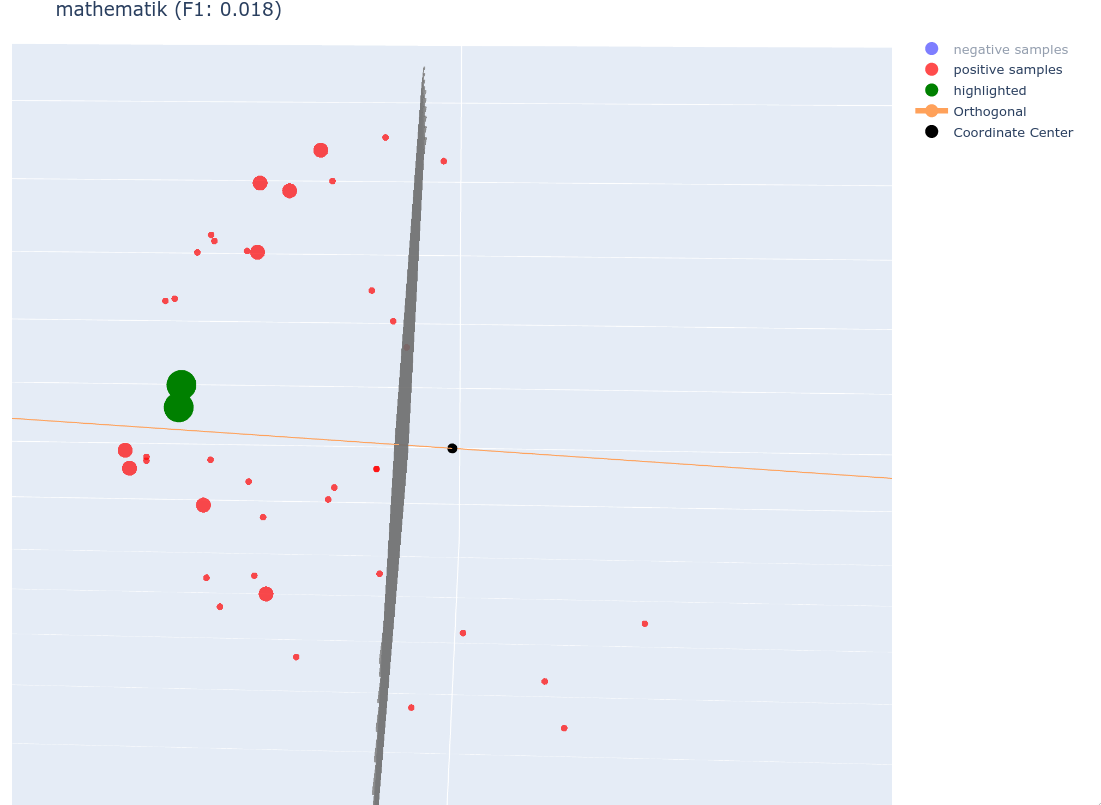
\includegraphics[width=\figwidth]{svm_mathematik_highlight_infoAB.png}
	\caption[3D-Plot with an SVM for the term \textit{mathematik}.]{
		\label{fig:3dplot_mathe_infoab}
		3D-Plot with an SVM for the term \textit{mathematik}, also highlighting the courses \textit{Informatik A} and \textit{Informatik B}. Negative samples are hidden for better visibility, and entities that contain the word more often than the 75\textsuperscript{th} percentile have bigger markers.
	}
\end{figure}

\autoref{fig:3dplot_mathe_infoab} displays a 3D-Embedding for courses, splitting courses which contain the term "\textit{mathematik}" from those that do not, also hightlighting the courses \textit{Informatik A} and \textit{Informatik B}. Both courses are close to each other for both the \textit{normalized angular distance} and also euclidean distance.\footnote{Normalized Angular Distance: Average 1.00, Info A and Info B: 0.37 (Percentile 8.2), Euclidean Distance: Average 0.88, Info A and Info B: 0.39 (Percentile: 8.9)}
Further, even though neither course description contains the word \textit{mathematik}, both courses would receive high values for this feature, indicated by the distance to the decision plane.\footnote{Both statements are better visible in the interactive version of the plot}

% * Seems to be the case, also nice that they are on the mathy side
% * Also holds for other stuff like language ourses, mathe für anwender 1 und 2, etc.

% \subsubsection*{Robustness}

% bei mir halt einfach für die verschiedenen configs laufen lassen, die resulting direction clustern und counten wie viele verschiedene terms vorkommen (gehirn vs psyhologie), ob einige besonders oft rauskommen und wi nah (cosine) die sind -> ROBUSTNESS ASSESEN

% How many unique in sum are there (out of 53 possible)

% Mathematik/Informatik: 22,
% Wirtschaftswissenschaften: 34,
% Rechtswissenschaften: 18,
% Sprach-/Literaturwissenschaften: 23,
% Humanwissenschaften: 23,
% Biologie/Chemie: 35,
% Physik: 37,
% Kultur-/Geowissenschaften: 21,
% Erziehungs-/Kulturwissenschaften: 29,
% Sozialwissenschaften: 29


% \autoref{tab:highest_ranking}

\subsubsection*{Are top ranking courses for the directions convincing?}

To further analyse the quality of the results, we are interested in the top courses of those directions that best represent the different faculties. \autoref{tab:highest_ranking} displays the most prototypical examples for each of those, which is directly derived from the rankings induced by the classifier.

\begin{table}[H]
	\makebox[\textwidth][c]{
	\resizebox{1.1\textwidth}{!}{%
	\begin{tabular}{@{}rcl@{}}
	\textbf{Faculty} & \textbf{Top Direction} & \textbf{Top Course for Direction} \\
	\midrule
	\textbf{Erziehungs-/Kulturw.} & \specialcell[c]{erziehungs-\\wissenschaft} & BA GM 3.2: Der Kinder Zukunft aus elementarpädagogischer Sicht \\
	\textbf{Rechtswissenschaften} & schuldrecht & Strafprozessuales Ermittlungsverfahren, [...] \\
	\textbf{Wirtschaftsw.} & fallstudie & WIWI-B-18001-WI: Management Support Systems B I (BI-Praktikum SAP/BW) \\
	\textbf{Kultur-/Geow.} & stadtgeographie & Mittelseminar/Angewandtes Seminar: Geographische Handelsforschung [...] \\
	\textbf{Mathem./Informatik} & mechanik & Technische Mechanik IV für Maschinenbau \\
	\textbf{Sprach-/Literaturw.} & \specialcell[c]{deutschen\\literatur}  & Deutsch - diachron: Historische Linguistik und Sprachwandel in der Gegenwart [...] \\
	\textbf{Humanwissenschaften} & gehirn & Willensfreiheit und Hirnforschung [...] \\
	\textbf{Physik} & klar & B1-B2 Schwedisch Erweiterungskurs: Schweden - das Land und die Menschen (DIGITAL) \\
	\textbf{Biologie/Chemie} & stattgefunden & Transformation wohlfahrtsstaatlicher Regime in Europa: Aktuelle Forschungskontroversen \\
	\textbf{Sozialwissenschaften} & parteien & Modul Vergleichende Politikwissenschaft I: Westliche Regierungssysteme im Vergleich \\
	\end{tabular}
	\caption{Highest ranking courses per feature that best predicts the faculty.}
	\label{tab:highest_ranking}
	}}
\end{table}

Again we observe that many of these make intuitive sense, but \textit{Physik} and \textit{Bio/Chemie} cannot be satisfactorily captured by our dimensions. \textit{Mechanik} was an unfortunate choice to encode \textit{Mathematik/Informatik}, however the corresponding course for the \textit{direction} definitely seems resonable.


% \paragraph{concluding remarks}

% In general we must say that we have really good accuracies and this really seems to indicate that it works.  We could to the shallow-decisiontrees-thingy for other attributes of the dataset than we currently have (see future work)

\subsection{Hyperparameters results}

After much preliminary elimination of other techniques, we decided on 165 different hyperparameter-combinations for the final run, which are what was decided on in after much preliminary elimination of other techniques.\footnote{An exception to this are of course the results for three dimensional spaces, which are not competitive and only generated because they are more intuitive and presentable.} For example, prior experiments have shown that the \textit{reclassify} algorithm to find cluster directions outperforms the one used in \cite{Derrac2015}, which is why the latter was not considered in the final evaluation, to counteract a combinatorical explosion of hyperparameters.\footnote{With regards to this specific parameter, there is however qualitativ evidence given in \autoref{tab:text_per_dim}.}

\paragraph{Classifier-Scoring-Methods}

Let us first consider if the choice of the exact evaluation method to quantify the classifier performance is relevant. For that, we look which score leads to the best result, and if the results differ drastically. \autoref{tab:kappa_table} clearly indicates that the algorithm is very susceptible for the exact scoring method used. It was to be expected that comparing raw counts to rankings performs worst (column \textit{c2r+}), and that was confirmed. Besides this, it is also interesting how big the difference between \textit{rtr2+min} and \textit{r2r+max} is, considering that they only differ in how they deal with duplicates. It was suprising that \textit{digitizing} the values 
worked at all. We see that the only scoring-methods that produced enough (2*\#Dims) cluster-centers are those that only considered those terms that occur at least once, which makes sense given that otherwise the scoring was too much influenced by the number of elements in the positive class. 

To get a better grip on the algorithm's robustness with respect to the exact scorer choice, let us now also consider their overlap as printed in \autoref{tab:kappa_overlap}. %\todoparagraph{Was waren die anderen hyperparams fur diesen run???}

Some things we see include:
% \todoparagraph{Yo chris diese interpreationen kommen von ner alten version der tabelle ups !! NOCHMAL ANGUCKEN!!}
\begin{itemize}
    \item binary kappa and F1-score have a high overlap (kappa being a bit stricter)
    \item comparing rankings of only the positive values and their digitized versions leads to the exact same results
    \item all of r2r+min/dig+2, kc2r+ are in b2b
    \item all of the onlypos-statistics are completely in the respective kappa bin2bin
\end{itemize}

Furthermore, looking at the individual scoring methods also provides insight with regards to the question if the different nature of our dataset needs to be accounted for: As established, a very important difference is that more relevant words do not occur more often in the Siddata-dataset. This makes it a reasonable assumption that scorers that evaluate the \textit{rankings} should perform worse: If it is not the case that important words that are very relevant to an entity necessarily occur more often in its associated text, comparing its ranking should perform worse than considering the classification as a binary problem. 

We can test that by comparing the overlap of features that achieve high kappa-scores with those that achive high scores of binary metric such as \textit{accuracy, precision, recall} and \textit{F1}. \autoref{tab:kappa_overlap} indicates first that the binary metrics are a lot less strict than the kappa-scores: All those terms which exceeded the threshold of 0.5 for one of the kappa-scores also did so for accuracy and recall. For \textit{precision} and \textit{F1}, however, this is not the case. More evidence is that the kappascores are a lot worse on count than they are on \glspl{quant}. Furthermore, the kappascores are a tiny bit better on lemmatization than without it, providing even more evidence, as it is to be expected that this configuration has a slighly higher word count.
 
\paragraph{Other Hyperparameters}

Note that the results reported in \autoref{tab:kappa_table} were considered \wrt deciding which ones to take for the final runs. This refers only to the decision which scoring methods to use but also about the hyperparameters up to that point - if not at least 2*ndim candidates for clustercenters are generated, the config is useless. In fact, it can be assumed that more extracted values are generally better, because if only the minimal number is generated all of them will become cluster center no matter their degree of collinearity, which makes the resulting space useless. With that in mind, \autoref{tab:kappa_table} suggests that a parameter-config with 200 dimensions that \textit{tf-idf} will tend to produce most dissimilar candidate directions.

In general, the results for different hyperparameters in terms of classifier performance (\autoref{tab:best_params}) indicate some trends:

For one, it definitey shows that comparing the raw count with these rankings performs worst, indicating that while the wording in \gencite{Derrac2015} was ambiguous, they likely talked about comparing the respective ranks. The second predictor of below-average scores is the usage of a three-dimensional embedding. This was to be expected, and given the low expressive power exptected from a three-dimensional embedding, the observed scores are even surprisingly high.

Comparing PPMI and tf-idf as scoring methods does not show any clear trends, however we can also not find good reasons to prefer the former over the latter. Given that calculation of PPMI-scores relies on huge matrix multiplications which are computationally inefficient, we would suggest to use the well-known well-optimized tf-idf score instead. Another insteresting observation is that scoring the Candidate-Matrix differently than frequency matrix of the texts is competitive with using equal scorings for both. Also, even using the raw count for the candidate-matrix did not perform very badly, serving as our final piece of evidence to see the robustness of the algorithm for datasets like ours.

Besides these observations, the other hyperparameters did not seem to affect classification performances much. In the printed table, the highest score is yielded by a 200-dimensional embedding with tf-idf encoding. However the results slightly varied for different random seeds due to differing elements ending up in the train- and test-set, leading to slightly different results with another hyperparameter-configuration ending up slighly better than the one printed in this thesis.

% * interstingly, even with ony 3 dimensions we extract hundreds of params (wtf - doesn't the later table say 3d always sucks?)


% Im allgemeinen muss man sagen die waren nicht so wichtig. When , what config we received was really mixed, sometimes 50d was best, sometimes 200d. 

% * The calculation How to find the best threshold for candidates
%     * did the threshold help?

% \todoparagraph{As exptected, 3D is not too good, and we see that the best combination is blablabla}

% \todoparagraph{What do we see? We see that tfidf is besser than ppmi blablabla}


% \includeMD{pandoc_generated_latex/5_hyperparamresults}


% So what else do we see in the hyperparams?
% * obviously 3d is worst, often didn't even have 6 values with kappa > 0.5
% * Did lemmatizing help?
% * was ppmi better than tf-idf? on par? worse?
% * was the 80 words threshold good?
% * were we correct in assuming that accuracy may be better than kappas? (no)

% TODO: generally write about if Kappa is a good choice (see eg \url{https://en.wikipedia.org/wiki/Cohen%27s_kappa})


% \subsubsection{Our algorithm improvements}

% our reclassify is better tan the desc15-algo (\ref{tab:text_per_dim}).

% \todoparagraph{The different find-name-was??}

% we wrote before that "taking all words as candidate and running a \gls{pos}-tagger led to suboptimal results in previous experiments, which indicated that the robustness of the algorithm is increased if less candidates are used. This will be forther elaborated in the discussion." -> say something about the number of candidates and how its better the way we do it.



% \subsubsection{Robustness}

% first is nsamples, second is maximal number, last is max number
% For 50D:  38 3800 1003
% For 200D: 15 6000 1707


% Robust meaning here that multiple runs yield similar results. We said before that in word2vec the actual directions of the vectors are completely incomprehensibly dependent on the random initial conditions, and we also said that that is an absolute no-go in conceptual spaces.

% Already here go into detail how unrobust the implementation of derrac and the others is. 

% Show and interpret results for how robust my implementation is and if close words are close

% ..then again elaborate that explicit word choices are not too relevant and also not tested here and that we already experimented with different techniques (see appendix for keybert vs the others) but that there is no formal way to test them.

% We hypothesize (see \autoref{sec:extract_cands}) that the reason we are having more robust results than \cite{Derrac2015} is among others because we have less candidates.

% Results of multiple runs: 

% from all the 165 different param-kombis we did, the following had enough (ndims*2) kappas-over-0.5:
% \{3: 40, 50: 38, 200: 15\}

% \subsubsection*{Stuff that we could have done}

% Are the phrases making up the semantic-direction-clusters similar?
% Are there dimensions encoding the COVID-19 pandemic?
% Is there a direction capturing advanced courses?
% Nen Plot der closeness im embedding mit levensthein-distanz und anzahl-gleicher-wörter korreliert und schaut wie explainable das ist

\vspace{-1ex}
\subsection{Did we achieve the thesis goal?}

Let us now take a step back and answer the question if the results indicate that we achieved the aims of this work. For one, there is certainly more work to do to increase robustness of the results in the sense that an unambiguous name for the resulting semantic direction comes up without being affected much by precise hyperparameter choices or random seeds. The fact that we have tested only by comparing how good the classification can be predicted is also a drawback, but a human study would be clearly outside the scope of this work.

Our results and analysis reach all expectations set in \autoref{sec:success_conds}: We have extensively analysed the difference between the Siddata-dataset and the originally used dataset. Though many differences between the datasets have been found, it has been shown that the algorithm can make sense of the dataset regardless. All results printed in this work are open-source and the original notebooks are freely available to prove that we did not cherry-pick any results for the analysis performed of the previous section. The semantic directions we have found allow to predict a courses' faculty, which encodes an important feature for the recommendation of educational resources. Our performances to predict the faculty even outperforms a classification relying on \gls{bert}.

% \includeMD{pandoc_generated_latex/5_2_siddata}

\section{General Algorithm}

% Now that we seen the algorithm in action and painstaking implemented it we are experts on the algorithm of \textcite{Derrac2015}, so let us critically reflect on the algorithm as such.

After having presented and meticulously implemented the algorithm of \textcite{Derrac2015}, we are familiar enough with the relevant theory and practice, allowing us to now critically reflect on the algorithm in general.

\subsection{Algorithm idea}

When first looking the algorithm of \textcite{Derrac2015}, it appears astonishingly specific. However after having read Gärdenfors' book \textcite{Gardenfors2000a}, the idea for their algorithm is self-evident: In it, Gärdenfors suggests that conceptual spaces can be generated from high-dimensional sensory input by using \gls{mds} to project the original data into a Euclidean space to do geometric reasoning in that space. The book has an entire chapter on computational aspects, in which the author discusses vector space models, dimensionality reduction techniques an \gls{ann} architectures for different levels of human conceptualization. According to that, MDS is especially good at dealing with pairwise distances judgements from a subject's perception, to create a more \textit{economic} representation for \textit{phenonemal} \glspl{cs} \cite[221]{Gardenfors2000a}. \textcite{Derrac2015} did not create the space from sensory data but from text corpora, where the distance of two texts can be measured by the words they share. Their algorithm reasonably combines the idea to generate \glspl{cs} with the steps for a classical \gls{nlp} pipeline as described by \cite{Turney2010} (\autoref{sec:vsm_construction}) Given that, the core contribution of \cite{Derrac2015} mainly lies in the idea that the \textit{faithfulness} of a potential direction for the resulting semantic space can be assessed by the performance of the corresponding decision problem.

\paragraph{Measuring the Faithfulness of directions}

It seems reasonable that this assumption holds for the datasets originally considered by \textcite{Derrac2015}. As extensively discussed, when concatenating reviews of movies or tags describing pictures of places it is natural that words that describe a salient feature of the respective entity occur more often. The Siddata-dataset consists of short descriptions without this property, where most words have a relative document-freqeuncy of less than a percent. However, the technique of comparing the ranking induced by the classification with the score of the words still yielded enough results, and the directions seem to consist of interpretable properties. This surprisingly confirmed the robustness of the algorithm in that regard.

% Under the assumption of the \gls{distribhyp}, the assumption that this is possible seems reasonable. \todoparagraph{Naher drauf eingehen warum? Ich kann nicht einfach distributional hypothesis sagen und fertig}

\subsubsection{Requiring MDS}
\label{sec:discuss_mds}

\textcite{Derrac2015} explicitly state that MDS is the best dimensionality reduction technique for their algorithm, as it is one of the few ones that result in a metric space. In their paper, they describe SVD (the mathematical algorithm behind \gls{lsa}) as a popular technique for dimensionality reduction, but further state that \q{SVD produces a representation in which entities correspond to vectors, which should be compared in terms of cosine similarity rather than Euclidean distance. [...] However, we can expect that spatial relations such as betweenness and parallelism [...] are not meaningful in the representations derived from SVD} \cite[14]{Derrac2015}. These relationships are required for semantic classifiers which mimic analogical and betweeness-based reasoning, which they demonstrate to work for all of their domains. However, this space does not have semantic directions. The \textit{final} feature-based representation of the entities is reached by ranking each entity for each of the feature directions and creating new vectors from these ranks. As acknowledged by \textcite[22]{Derrac2015}, the feature vectors are not orthogonal, not linearly independent and only of ordinal scale level, withhout meaningful distances. \textcite{Derrac2015} create semantic classifiers both for the \textit{intermediate} space with meaningful distances (geometric betweeness- or parallelism-based classifiers) as well as for feature-based representation (a-fortiori-classifiers, see \autoref{sec:reasoning}). However, \textcite{Ager2018,Alshaikh2020} are only interested in the latter space and its resulting feature axes. If that is the case however, it becomes irrelevant if the intermediate space is metric or not, which enables for other algorithms to be used in that step. As stated in \autoref{sec:dim_red}, LSA may be the better choice as it explicitly detects latent topics in descriptions instead of relying on words that are explicitly mentioned. This may also lead to other desirable properties such as comparability of documents and phrases.

If for the explainable classifiers the relevant space is the one with semantic directions, geometric properties of the intermediate space are irrelevant. Instead one should try to generate a space that has both a useful metric \textit{and} interpretable directions. Depending on what the authors consider to be the end result of their algorithm, only one of these necessary requirements for conceptual spaces is fulfilled. So if their end-result is the intermediate space, that is nothing more than a normal \gls{vsm} with some interesting but long-term useless geometric properties. Instead, another possibility may be to calculating a new orthonormal basis on the coordinate system. The next step would then be to enforce orthogonality of the semantic directions as good as possible, and using linear algebra for a change of basis for the entites, such that not only their ranks but their exact position for each semantic direction (axis) is relevant. Subsequently, one could use techniques like Principal Component Analysis to decorrelate the directions. In this way, one would obtain vector without a name, which however could again be found with techniques that rely on \glspl{cos} such as LSA.

\textcite{Ager2018,Alshaikh2020} both do not this interim space and only use re-embedded one, but retain the use of MDS regardless. To our best understanding, they have no reason to do so, giving impression that they read to use MDS in Gärdenfors' book and then forgot that their final re-embedding step makes that irrelevant. 

\paragraph{Using classical techniques}

In fairness, \cite{Ager2018,Alshaikh2020} both experiment with modern neural embeddings for the entities such as averaged \gls{word2vec} or \gls{doc2vec}. Both authors report that this decreased performance (see \autoref{tab:f1_placetypes_long}) compared to their MDS-condition.\footnote{Even though \textcite{Alshaikh2020} state in their paper that relying on better embeddings such as \gls{bert} \cite{Devlin2019} may lead to better results.} However, while they use neural embeddings, they do not adjust any of the later steps to regard for that: they just replaced the \gls{vsm} generated classically in the first steps of the algorithm with a neural embedding, such as averaged GloVe embeddings \cite{pennington2014glove} of the words in the text. On that they ran the exact original algorithm of creating a frequency matrix from the \gls{bow} and using a linear classifier to get the direction. 

% \todoparagraph{Wenn man schon embeddings nutzt dann soll man auch die eigenschaft dass die sinnvolle richtungen haben nutzen. Und wenn man dann shcon mit vektoren arbeitet dann kann man auch lsa undso nutzen. Und dann hat man auch nicht mehr das problem mit too-small-positive-class}

They do not consider looking for latent topics or make use of the algebraic properties that are given for these embeddings (see \autoref{eq:w2vregularity}). A possible avenue could be to look for shared vector components of entity-embeddings and candidate-word-embeddings. Instead, they still rely on the usage of linear classifiers that split according to frequency matrices. We will look more detailed into that soon, but this makes much more sense for \textit{points} in Euclidean spaces than it does for \textit{vector} embeddings where the space is built up from a cosine-distance-similarity-based objectives (see \autoref{sec:mds}). Instead of that, it seems the better idea to take advantage of dealing with vectors, such as the fact that they are inherently directional already. As discussed in \autoref{sec:lsi}, it seems that the concepts of \gls{lsi} to compare the similarity of documents and candidate feature directions seems more appropriate. This has added benefit that not only words literally occuring in the respective texts can be considered, which among others counters the previously stated problem that the used classifiers deal with heavy class imbalance as well accounting for polysemy and synonymy.

% \removeMe{

% \todo 
% \paragraph{Other things}
% Their last step to cluster the good-kappa-ones is very basic and has much room for improvements, see my suggestions.
% Their merge-cnadidate-step (alle nehmen und die zum closestem herclustern und dann die richtung des $T^0.5$ übernehmen) also has much room for improvement, see my suggestion for another algo - we did implement already some stuff but many better ones are imaginable (see future work)
% better ways of getting rid of irrelevant clusters (see my suggestion and also problems with stopwords)

% They do one SVM per term and then cluster similar ones. Ther terms sometimes occur only in like 50/15000 entities, so the validity of the kappa is should be doubted. \cite{VISR12} and many others first try to find latent stuff, which would improve that by a lot because its a lot less sparse. ("contains-one-of-the-terms" is a lot more than "contains-this-term" - that knowledge is also used by the postprocessing of Ager even though shitty.). According to \cite{Derrac2015} there are no methods that keep a metric space, however as discussed for our aim we can drop that.

% \paragraph{Robustness}

% \todoparagraph{We discussed Robustnes before!}
% An algorithm that is so unrobust \wrt its precise parameter-choices seems a bad choice for conceptual spaces in general. A big issue why we disregarded VSMs is because of their arbitrary dimensions!

% }

\subsection{Does the algorithm actually produce a Conceptual Space?}

\autoref{sec:cs} explained what a conceptual space is, before introducing \gencite{Derrac2015} algorithm to automatically induce them. However, their algorithm only approximates \glspl{cs} and does model some parts of the definition. A first difficulty with the algortihm is, that it needs a clearly defined domain from the start. It takes a corpus of texts and embeds each of these into a single high-dimensional vector space. If not all texts in the corpus are from a single domain, due to the similarity-based vector space generation, outliers will greatly affect the embedding of all entities (as \cite{Ager2018} discusses at length). This sounds irrelevant in practice, but the problem is that it is impossible to clearly define what a domain is. There is the set of place types, but this domain consists of various subdomains, and some concepts apply only to a specific subset of entities. The described algorithm cannot figure out such subdomains. This issue is partially addressed by the works of \textcite{Alshaikh2019, Alshaikh2020, Alshaikh2021} which elaborate on the idea of subdomains. As they state, \textit{\q{When representing a particular entity in a conceptual space, we need to specify which domains it belongs to, and for each of these domains we need to provide a corresponding vector.}} \cite{Alshaikh2020}\footnote{Their improvement to the work of \textcite{Derrac2015} is many to introduce the concept of sub-concepts to the algorithm by hierarchically disentangling the generated space into subfeatures that only exist if certain top-level features are given, such as encoding the \textit{political orientation} of Organizations only for those have a high degree of being \textit{political} in general.} 

Also it is important to be aware of the difference between what \mainalgos and this work consider a domain (the set of movies, places or courses), and the definition of domain as used by \textcite{Gardenfors2000a}. According to the latter, a domain is a low-dimensional set of correlated properties, such as \textit{the color domain} consisting of \textit{hue, saturation} and \textit{value}. This also points out another difference of the original \gls{cs} definition and the definition used here: Conceptual spaces describe an entity through several uncorrelated low-dimensional vector spaces, not a single one with several dozen dimensions. As \cite{Ager2018} puts it more humbly, \textit{\q{The idea of learning semantic spaces with accurate feature directions can be seen as a first step towards methods for learning conceptual space representations from data [...]}}. Again it is referred to the works of \textcite{Alshaikh2019, Alshaikh2020, Alshaikh2021} which alleviate this by iteratively finding disentangled low-dimensional feature spaces.

As discussed earlier, the algorithm of \textcite{Derrac2015} first embeds the entities into a Euclidean space where the concepts of betweeness and parallelism make sense, and subsequently create a feature-based representation that bases on an entity's rank \wrt several human-interpretable features. The final embedding is only of ordinal scale level and thus unable to model  degrees of similarities. In other words, the algorithm produces \textit{either} a space with a euclidean metric, \textit{or} one with interpretable directions, but no space that has \textit{both properties}. As both are necessary conditions for a conceptual space, \gencite{Derrac2015} algorithm at no point generates something that resembles a \gls{cs}. It remains unclear to us why they only consider the ranking of the entites regarding the feature axis instead of their distance which may retain relations of distances, for example by applying an arithmatic change of basis for the coordinate system (linear transformation). The way their algorithm works, the final space only has ordinal scale level and linearly dependent (correlated) dimensions. An interesting research avenue is to figure out what properites the space they have, and if small changes to the final algorithm step (such as \gls{pca} to decorrelate dimensions or not only taking the rank) could help in retaining the euclidean or at least another usable metric.

\subsubsection*{Points instead of Regions}

Another important difference between the resulting space and \glspl{cs} is that we are dealing with points instead of regions. Advantages of doing that include that it allows to distinguish \textit{protypical} examples from borderline cases \cite{Gardenfors2000a} and straight-forward application of ontological relations through the \gls{rcc} (see \autoref{sec:ontology_rcc}). \textcite{Derrac2015}, however, drop this assumption and work with vectors instead of regions, claiming that this is a \q{coarse-grained approximations of conceptual spaces, where points correspond to fine-grained categories instead of specific instances, while convex regions are used to model higher-level categories} \cite[8]{Derrac2015}. Despite that, they never address it again, so in the end they stick with points. This breaks with one of the key concepts from \glspl{cs} and also renders it impossible to simulate any of the ontological relations with the resulting spaces, which Gärdenfors considered their most relevant practical application \cite{Gardenfors2004}. 

However, when elaborating on the idea that conceptual spaces can be induced using Kohonen-Nets (\autoref{sec:algo_variants}), Gärdenfors himself claims that mapping regions of the original space to point-embeddings in the \gls{cs} is an \textit{advantage}, because it resembles \textit{generalization}. Another aspect to consider is whether the \glspl{entity} as considered by \mainalgos actually resemble what Gärdenfors originally considered an entity. The entities in the used datasets of educational resources, placetypes or movies actually are specific instances instead of general \textit{concepts}. Instances in a conceptual space are correctly modelled as points - one could say that regions denote \textit{types}, with the individual points corresponding to their \textit{tokens}. Considering that we have only one instance per entity, we are dealing with types. Concepts (Regions in a CS) could accordingly be induced as the set of multiple tokens. A practical implementation could, for example, model the concept of \textit{introductory computer science courses} as a convex region spanned by all of the instances it contains. \textcite{Erk2009} propose an algorithm that creates such a region with varying variances per dimension from a set of prototypical instances. It should be noted, however, that learning boundaries for such regions requires much more data \cite{Derrac2015} and the aforementioned reasoning on regions is computationally very complex \cite{Hernandez-Conde2017}.


\paragraph{Vectors or Points}
\label{sec:discuss_points}

The authors explicitly claim that they are dealing with points in a Euclidean space, which should be compared in terms of Euclidean distance \cite[14]{Derrac2015} instead of \gls{cos}. Despite this, in the merge-canidates step of their algorithm (\autoref{sec:algo:cluster}), they compare the candidate feature directions using the \gls{cos} of their orthogonals. As they require similarity of directions and not of positions, this approach seems plausible. However, these vectors do not have their origin in the coordinate base but in the position where they cut across the SVM's decision surface: A SVM is described by the vector of its orthogonal intercept, a scalar describing where the decision hyperplane crosses it. This means that one is dealing with \textit{affine frames} (which are described by basis and origin) instead of vector spaces. However, vectors in affine spaces cannot be compared solely by the angle between them\footnote{For better comprehension it is referred a StackOverflow question of \me at \url{https://stackoverflow.com/a/69407977/5122790}}. The way their algorithm is described, their merging of feature direction disregards the origin. Consider the following example: The SVMs for two candidates have exactly the same orthogonal vector, but different intercepts. There might be samples between the two decision surfaces, which are classified towards the positive class by the one classifier, and towards the negative by the other. If they classify samples differently, they must express different concepts. When only accounting for the direction of the orthogonal, such information gets lost. 

\subsection{Outlook}

There are also techniques that extend the algorithm of \textcite{Derrac2015}: \textcite{Alshaikh2019} take a vector space embedding and decompose it to several low-dimensional spaces, such that it corresponds more closely to the definition of a \gls{cs} which are split into multiple domain-specific spaces of low dimension. For that, they take the spaces from \cite{Derrac2015} to then cluster their features by domain and iteratively remove these groups to create multiple subspaces, while ensuring that \gls{word2vec} embeddings close to those of the removed ones are disregarded for future features.

\textcite{Alshaikh2021} want to get rid of MDS with its quadratic space complexity and also write a completely new, unsupervised ANN algorithm based on GloVe embeddings \cite{pennington2014glove}. In it, they learn domain-specific embeddings from the BoW and like \cite{Derrac2015} use classification, splitting entities that contain one of the verbatim candidates vs. those that do not. They train an \gls{ann} on this while also punishing close embeddings, similar to their previous work \cite{Alshaikh2019}.

% \subsection{Regarding their research practices}

% In \autoref{sec:howtoreplicate}, we stated the importance that all claims made in research should be reproducible and testable. While replicating the work of \cite{Derrac2015}some Questionable Research Practices came apparent. For example, 



% \paragraph{Robustness}
% \todo

% \paragraph{Ambiguity}
% \todo




% \includeMD{pandoc_generated_latex/5_3_evalderrac}




\section{Architecture}

As one of the thesis goals asked for a good and scalable architecture, we will also evaluate whether the implementation fulfills the set criteria (\autoref{sec:success_conds}) and if the aspects we considered for a qualitative software and sustainable data analysis (\autoref{sec:reproducibility}) are fulfilled.
% We remember, we also wanted to build a good architecture and set goals for that, such as adaptability to new datasets etc. We said a good architecture would show in adaptability, scability, ..., so we wanna show that these are achieved. 

First of all, we wanted to show that this implementation works and is able to replicate the results of one dataset of \mainalgos. This aim was reached, indicating \textbf{Functional Suitability} of our implementation and also the \textbf{Reproducibility} of the original algorithm.\footnote{If our implementation itself is reproducible can hardly be shown by \me in this thesis.}

Another goal was that the code-base successfully runs on the \gls{ikw} compute grid. This goal was also met, and the resulting implementation and its \textbf{Automation} and \textbf{Scalability} proves satisfactory. Testing new hyperparameters is as easy as changing a YAML-file, transferring the file to the grid and executing a command\footnote{such as \codeother{MA_ENV_FILE=siddata.env submit by_config --configfile config/CONFIGFILE.yml}}. The maximum number of cores per node and of nodes available to a user (64) are maximally utilized, which also indicates optimal dependency resolution. Running the algorithm on sample datasets worked without any complications in a matter of minutes (\textbf{Modularity, Maintainability, Adaptability}).

Allowing for all this was surprisingly intricate. Having worked with \textit{Snakemake} on clusters before, the amount of customization to allow for workflow management on the \gls{ikw} grid was surprisingly high. This was partially due to heavy iterative restructuring of the code-base to comply with the logic as demanded by this workflow management system. Part of this is due to peculiarities of its configuration,\footnote{For example that \textit{accounting files} that keep track of jobs are inaccessible to users, which means that our scheduler needs to simulate their behaviour.} but also to a huge degree due to the walltime-limit of 90 minutes. Because of this, most of the algorithm components need to be written in a way such that they both massiveley parallelize, but also gracefully end and store interim results, and the scheduler must comply with this. Comparing this with the uploaded implementation of \cite{Alshaikh2020}\footnote{\url{https://github.com/rana-alshaikh/Hierarchical_Linear_Disentanglement}}, which consists of one Jupyter Notebook and one Python file, gives indication of the amount of work necessary to reach this. We sincereley hope that this thesis helps in \textbf{Transparency} and that at least the cluster execution will be re-used by other students of the \gls{ikw}.

All the analyses that were conducted for this thesis are given in the accompaning source code. All plots and tables from all previous sections that were not reprinted were created in publicly available Jupyter-Notebooks, together with many more analyses that were conducted but would go far beyond the scope of this thesis. All plots and tables are explicitly linked and easily re-creatable and runnable. A lot of work was put into the architecture, and as soon as architechture and worklow management worked as intended, further development on the algorithm was suprisingly quick. This indicates that the general aim of creating an architecture that helps to answer related future research questions is fulfilled. For the sake of brevity, this analysis and the code-base itself, which is available at \url{https://github.com/cstenkamp/derive_conceptualspaces} shall suffice as explanation regarding the final two set goals. 

% \removeMe{
%     \todoparagraph{IN 3_3_architecture is a section} "My workflow to generate results", darauf nochmal eingehen und sagen dass das wirklich wunderbar funktioniert, dass es am ende nur ein wenig chaotisch ist weil man darauf achten muss dass man consistent ist in den conditions für best-config (random seed für die decision trees undso)
% }


% \includeMD{pandoc_generated_latex/5_4_architecture}

\section{Future Work}
\label{sec:futurework}

While this work has shown that the general technique seems to work, so far it has not produced an actual recommender for edcucational resources. Accordingly, building an interface as \eg the one from \autoref{fig:movietuner}, or alternatively a textual interface that relies on a dialogue with a user to generate recommendations is an important direction for future work. When this is added to the Siddata-\gls{dsa}, this may directly be combined with a study in which the users volunteer information about the usefulness of recommendation or even providing possible labels, which may be used for algorithm evalution with labels other then the faculty, or even supervised training as done \eg by \cite{VISR12}. Also, more analyses can be performed on the current data, such as correlating distances in the semantic space with \textit{Levensthein-distances} in textual descriptions, or looking \textit{in what direction} individual faculties differ.

\subsection*{Algorithm Addendums}  As stated many times by now, the algorithm that was replicated in this work is very modular and requires only certain types of algorithm for many of its components. While recreating the works of \mainalgos, many smaller and larger changes to the algorithm could have been performed. A complete list of considered algorithm-extensions can be found in this repository\footnote{\url{https://github.com/cstenkamp/MastersThesisText/blob/master/pandoc_markdown_base/futurework_long.md}}. Among others, not all extensions from \cite{Ager2018, Alshaikh2020} have been implemented yet. It may also be insteresting to consider new distance-measures for the entities such as variations of the \textit{Levensthein-distance} or the \textit{Jaccard-distance} (\eg \gls{iou}, as done in \cite{Schockaert2011}). Also, more work is needed to remove irrelevant dimensions, in the hope of making the algorithm more robust. Especially the clustering and merging of similar features may benefit from considering other techniques. These include using \gls{iou} similar to \cite{Alshaikh2019} as similarity measure, methods to remove uninformative clusters, or considering other algorithms for clustering and calculating the centroid directions that weight or threshold based on classifier performance or similarity. Finally, finding a representative cluster name may benefit in robustness from also considering pseudo-documents \cite{VISR12} or other methods, \eg those suggested by \textcite{Carmel2009}.

\subsection*{Complex Changes} Besides the aforementioned additions, there are also many avenues that change more of the algorithm's logic. These include the fine-tuning step of \textcite{Ager2018}, which may be combined with latent topic detection techniques to alleviate the fact that the desriptions of the Siddata-dataset are short and omit many words that may serve to describe an entity. Many other ways to find latent topics may also be considered, such as relying on semantic databases and counting \textit{hyponyms} of candidate directions towards their count for a description, or again relying on vector similarity as demonstrated in \gls{lsa} and also neural embeddings such as \gls{word2vec} and \gls{doc2vec}. We have established that the current form of the algorithm only yields either a space with a Euclidean metric or one with semantic directions. Finding ways to get both would be an important contribution - it is \eg unclear why so far only rankings have been considered instead of linear algebra to find a new coordinate base. Alternatively, one can ignore the requirement of the Euclidean metric completely, which opens up many major changes to the algorithm such as not relying on \gls{bow}-representations at all, but instead using modern document embeddings such as \gls{bert}, where candidates are detected using the \gls{cos}.

\subsection*{New Algorithm}

Finally, let us try to combine all the issues raised in this work to form a suggestion of how a completely different algorithm may look.
First, we want an embedding that retains as much of the original dataset variability as possible. For that, additionally to a small set of absolutely most important dimensions found as the orthogonal of the linear classifiers, one may consider subsequently running \gls{pca}\footnote{PCA is a technique used for dimensionality reduction that works by projecting high-dimensional data onto its \textit{Principal Components}, those directions that explain most of its variance.} to find \textit{remaining} variance for those dimensions that do not obviously correspond to the occurance of single words. This has the additional benefit of finding \textit{orthogonal} directions which helps to get low-dimensional spaces, expressed by a small amount of uncorrelated features. So far, the directions found by \gls{pca} do not have a name, but we have also examined ways such as LSA that find words by their similarity of angles. In fact, it may be possible to build the whole algorithm on the basis of \gls{pca}: Instead of relying on \gls{bow}-representations, texts could be embedded using \eg \gls{bert}, which also takes into account its hidden topics and word ordering. Subsequently, one may run PCA to find a few directions of this space that best explain the dataset variance. Embracing the fact that one is dealing with vectors, \gls{lsa} can then be used to find candidate dimension names which do not rely on exact phrasing of the corpus. A disadvantage of such an algorithm is, that the resulting space is not metric\footnote{Though one may try to use pairwise distances for each of the dimensions to create a new metric space using a variation of MDS, or rely on Kohonen-Networks for that, as suggested by Gärdenfors \cite{Gardenfors2000a}.} - but neither is the space yielded by the algorithm explored in this thesis.



% \includeMD{pandoc_generated_latex/5_0_futurework}

\section{Conclusion}

This thesis explored how explainable generation of educational resources can be generated in a data-driven manner from a corpus of their descriptions. It has been established that \textit{Conceptual Spaces} can serve as knowledge representation method for that by capturing dataset properties in a way that allows to computationally model explainable reasoning. To generate these automatically, the method by \cite{Derrac2015} was thoroughly examined in theory and in practice.

The introduced algorithm was successfully replicated and the results on the originally used data have been confirmed. We have sucessfully transferred the algorithm to the domain of educational resources and demonstrated its ability to find relevant human concepts in our dataset. By means of this, we have demonstrated the robustness of the methodology by discussing the difference in the datasets as well as the respective results. Some adjustments to the original algorithm have been shown to further increase its performance. Analysis on the results of our dataset has shown that surrogate metrics indicate that the algorithm finds some regularities in the dataset, such as a courses' faculty. Despite this, more work to thoroughly test the algorithm's capabilities, but also to increase its performance and robustness will be needed.

To make the replication and application of the algorithm possible, we have implemented a tool that allows to easily recreate the results of \mainalgos. This tool was built while ensuring to comply with code quality standards and proper methodology, is open-sourced and can easily be installed as a package. The result of this is a reliable pipeline that has been demonstated to be easily adaptapted and extended. We hope this helps raising the attention of a broader community to the methodology and enables future research on further varition or domain transfers to be simple, quick and accessible. Another major contribution of this thesis are the solutions that were found to run workflows similar to the one required here on compute clusters, specifically the \gls{ikw} grid. The result is a workflow that is much more versatile and user-friendly than the ones we know to be used to date,\footnote{So far, the only methods that we have seen suggested are to write custom shell-scripts, see \eg the discussion and links in its respect Stud.IP group at \url{https://studip.uni-osnabrueck.de/plugins.php/coreforum/index?cid=e946790f6a74e17df02a85847b2110ab} \acc{04}{09}} and we hope that it helps to make high performance computing more attractive to other \gls{uos} students. All analyses conducted in this work are open-sourced as well and can be easily inspected and re-created.

Finally, we have discussed Conceptal Spaces and \gencite{Derrac2015} algorithm extensively on the basis of our results. We have reached the conclusion that while the algorithm produces reasonable results automatically and shows much potential, it drops necessary assumptions of Conceptual Spaces by not producing a single embedding that is both metric and also has interpretable dimensions. We have concluded that because of this, some assumptions about necessary design decisions can be dropped, which may allow to combine the methodology with state-of-the-art algorithms.

% * Wir haben diskutiert ob der algo sinn macht etc
% * Regaring CS: seems cool. Both in terms of  model of human concept formation AND algorithm-that-allows-certain-things-like-reasoning
% * Regarding the algorithm
%     * That motivated us in the first place: automatically create structured knowledge bases bc explainability. Need is there.
%     * I think it has potential
%         * Is it practical? enough so.
%         * though technically it doesn't create a CS - would be better if we can get both metric and interpretable direcitons. 
%     * I think better algorithms could exist, one should consider using neural embeddings.


% \includeMD{pandoc_generated_latex/5_6_conclusion}


% \chapter*{Acknowledgements}
%TODO A place to say thank you to everybody who helped you.

%=======================================================
% Glossaries


%TODO: If I don't want to have a COMPLETE pagelist, see https://tex.stackexchange.com/q/246818/108199
\renewcommand*{\arraystretch}{1.8}
\chapter*{Glossary}
\vspace{-5ex}
\addcontentsline{toc}{chapter}{Glossary}
\label{sec:glossary}
\glsaddallunused
\printglossary[type=defs,         title=Definitions, toctitle=List of Definitions, style=long3colheaderMINE, nogroupskip]
\printglossary[type=customs,      title=Custom Terms, toctitle=Custom Terms used in this thesis, style=long3colheaderMINE, nogroupskip]
% \printglossary[type=units,        title=Units,       toctitle=Units,      style=3colger]
\vspace{0.5cm}
\renewcommand*{\arraystretch}{1}
\printglossary[type=symbols,      title=Symbols,     toctitle=List of Symbols, nogroupskip]
\vspace{0.5cm}
% \printglossary[type=\acronymtype, title=Acronyms,    toctitle=List of Acronyms, style=2colacro, nonumberlist]
\printglossary[type=\acronymtype, title=Acronyms,    toctitle=List of Acronyms, nogroupskip] 


%----------------------------------------------------------------------------------------
%	THESIS CONTENT - APPENDICES
%----------------------------------------------------------------------------------------
	
	\appendix % Cue to tell LaTeX that the following "chapters" are Appendices
	\addtokomafont{section}{\LARGE}
	\addtokomafont{subsection}{\Large}
	\addtokomafont{subsubsection}{\large}


	\cleardoubleoddpage
	\phantomsection
	\addcontentsline{toc}{part}{\appendixname}
	\setchapterpreamble[o]{% siehe KOMA-Script-Anleitung
	\usekomafont{disposition}\usekomafont{part} \appendixname\bigskip} 	% the three above are to show the appendix as section, see https://golatex.de/viewtopic.php?p=22119&sid=ebe25f27fce1765ab7d8b1d2e91ee979#p22119

	% Include the appendices of the thesis as separate files from the Appendices folder
	% Uncomment the lines as you write the Appendices
	
	% Appendix A

% \newgeometry{
% 	a4paper,
% 	top=21mm,
% 	bottom=11mm,
% 	inner=24mm,
% 	outer=9mm,
% } %bindingoffset=.5cm

%\newgeometry{
%	a4paper, inner=1.9cm, outer=1.9cm, bindingoffset=1.3cm, top=1.5cm, bottom=1.5cm, 
%} %bindingoffset=.5cm


% \lstset{
% 	numberblanklines=false
% 	,basicstyle=\ttfamily%
% 	,breaklines=true%
% 	,tabsize=1%
% 	,showstringspaces=false%
% 	,numbers=left%
% 	,numbersep=\lstnumbersep%
% 	,numberstyle=\lstnumberstyle%
% 	,framesep=0pt%
% 	,xleftmargin=\lstnumberwidth%
% 	,framexleftmargin=\lsthorizontalpadding%
% 	,xrightmargin=\lsthorizontalpadding%
% 	,framexrightmargin=\lsthorizontalpadding%
% 	,backgroundcolor=\color{verylightgray}%
% 	,postbreak=\ding{229}\space%
% 	,escapeinside={*(}{*)}
% 	\linespread{1.0}
% }


\chapter{Code Use-Cases in Praxis} % Main appendix title

\label{AppendixA} 

\vspace{-0.8cm}

\label{ap:usecase_click}

\label{ap:usecase_snakemake}

\label{ap:usecase_notebook}

\includeMD{pandoc_generated_latex/6_0_usecases}

%\lstinputlisting[language=Python, firstline=29]{codes/dqn.txt}

 %have to use input and not include, otherwise the order of "Appendix" and the first appendix is wrong
	% Appendix B
% https://tex.stackexchange.com/questions/152829/how-can-i-highlight-yaml-code-in-a-pretty-way-with-listings

% \newgeometry{
% 	a4paper,
% 	top=21mm,
% 	bottom=11mm,
% 	inner=24mm,
% 	outer=9mm,
% } %bindingoffset=.5cm

%\newgeometry{
%	a4paper, inner=1.9cm, outer=1.9cm, bindingoffset=1.3cm, top=1.5cm, bottom=1.5cm, 
%} %bindingoffset=.5cm



\chapter{Implementation Details} % Main appendix title

A main goal of this thesis is to provide a code base that makes it as simple as possible to get started with \gencite{Derrac2015} algorithm to derive rudimentary conceptual spaces for any kind of dataset. In order to achieve this, documenting some implementation details and design decisions is crucial.
% TODO: something a la "es ist aber zu detailliert für den hauptteil und zerstört den lesefluss, deswegen ist der aufbau halt so dass der Hauptteil/der methods-section sich möglichst kurz fasst, wie halt die methods-section von nem Paper, und ebendieser appendix für diejenigen gedacht ist die den spezifischen Algorithmus genauer wissen wollen ODER den code nutzen wollen ODER sich einfach fragen warum dinge so sind wie sie sind. Also I HAVE to cite some of the used techniques as per their licences.
This appendix goes into more detail for selected components of the algorithm.

\label{AppendixB} 

\section{Algorithm Details}

\subsection*{Preprocessing}

see \autoref{sec:algo_preproc}

\subsubsection*{Language-Detection and Translation}
\label{ap:translating}

To check the languages of the entities, the \codeother{langdetect}\footnote{\url{https://pypi.org/project/langdetect/}, \textcite{nakatani2010langdetect}} library is used, which is a direct port of a java library that claims to have 99.8\% accuracy on longer texts \cite{nakatani2010langdetect}. 
\newline

Depending on the translation-policy, it is possible to either take only those entities of the demanded language, ignore it and consider all entities in their original language, or enforce the demanded language by translating all entities from their original language to the demanded one. The accompaning code for this thesis contains extensive code to do that using the \emph{Google Cloud Translation API}\footnote{\url{https://cloud.google.com/translate}}. Many descriptions of the SIDDATA-dataset were translated using this technique\footnote{As, however, only 500.000 characters per google-account and month can be translated \href{https://cloud.google.com/translate/pricing}{free of charge}, the translation-process for the descriptions is still in progress.}. As of now, Google's Cloud Translation Service uses an embedding-based neural model of a hybrid architecture that has a transformer encoder, followed by an RNN decoder \cite{Chen2018}. All of the languages detected in the SIDDATA-dataset are supported by the system - translating between the languages German, English and Spanish, which make up \todoparagraph{HOWMANY} percent of the SIDDATA-descriptions, is what the system is particularly optimized for. 
\todoparagraph{write short about their percentage, bleu score etc}

\includeMD{pandoc_generated_latex/6_1_implementationdetails}

\subsection*{Candidate Extraction}

see \autoref{sec:extract_cands}

\subsubsection*{KeyBERT}
\label{ap:details_keybert}

The \emph{KeyBERT}-algorithm\footnote{\label{fnote:keybertgibhut}\fullcite{MaartenGr2021}} \cite{grootendorst2020keybert} is one of the techniques used to select phrases of the text-corpus as candidates for \gls{feature}-directions. 

KeyBERT is a keyword-extraction technique \q{that leverages BERT embeddings to create keywords and keyphrases that are most similar to a document}\footnoteref{fnote:keybertgibhut}. \Gls{bert} is a neural language representation model that is able to embed both words and documents. Its embeddings are obtained by training a multi-layer bidirectional transformer encoder \gls{ann} architecture on a task in which a masked word must be predicted from the its bidirectional context as well subsequent fine-tuning tasks \cite{Devlin2019}. To extract keywords, the KeyBERT algorithm embeds both the document as well as its containing \glspl{ngram} of a configurable length using BERT and returns those phrases whose embedding ist most similar to the document-embedding according to the cosine-similiarity\footnoteref{fnote:keybertgibhut}.

The KeyBERT-model was incorporated to extract key-phrases for this codebase in two ways: 

\paragraph{KeyBERT-original} runs the algorithm on the unprocessed original texts. This is reasonable, as this is what BERT-embeddings are trained on, however it has the disadvantage that it requires a lot of post-processing to match the extracted phrases to the processed descriptions (which \eg may contain only lemmas or have their \glspl{stopword} removed)
\paragraph{KeyBERT-preprocessed} alleviates this problems by running the algorithm on already preprocessed texts. This may however lead to worse results, as the algorithm was trained on unprocessed natural sentences.

In practice, though both variants extracted different phrases, the results for either of the technqiues did not differ significantly.


\subsection*{Candidate Filtering}

\begin{table}[H]
    \centering
    \resizebox{\textwidth}{!}{%
    \begin{tabular}{llllll}
    \textbf{Long}                    & \textbf{Short} & \textbf{Data} & \textbf{Quantifications} & \textbf{Distances} & \textbf{Comments}                \\ \midrule
    rank2rank\_dense          & r2r-d          & all           & Dense-Ranked           & Dense-Ranked     &                                  \\
    rank2rank\_min            & r2r-min        & all           & Min-Ranked               & Dense-Ranked     &                                  \\
    bin2bin                   & b2b            & all           & Binary                   & Binary             & Disregards rankings              \\
    digitized &
      dig &
      all &
      Digitized &
      Digitized &
      \begin{tabular}[c]{@{}l@{}}Bins decided by np.histogram\_bin\_edges \\ from min and max of all data\end{tabular} \\
    count2rank\_onlypos       & c2r+           & positive      & Unchanged                & Dense-Ranked     & Only for Count as Quantification \\
    rank2rank\_onlypos\_dense & r2r+d          & positive      & Dense-Ranked           & Dense-Ranked     &                                  \\
    rank2rank\_onlypos\_min   & r2r+min        & positive      & Min-Ranked               & Min-Ranked         &                                  \\
    rank2rank\_onlypos\_max   & r2r+max        & positive      & Max-Ranked               & Max-Ranked         &                                  \\
    digitized\_onlypos\_1 &
      dig+1 &
      positive &
      Digitized &
      Digitized &
      \begin{tabular}[c]{@{}l@{}}Bins decided by np.histogram\_bin\_edges \\ from min and max of all data\end{tabular} \\
    digitized\_onlypos\_2 &
      dig+2 &
      positive &
      Digitized &
      Digitized &
      \begin{tabular}[c]{@{}l@{}}Bins decided by np.histogram\_bin\_edges \\ from min and max of all positive data\end{tabular}
    \end{tabular}%
    }
    \caption{Dense means: if there are 14.900 zeros, the next is a 1
    Min means: if there are 14.900 zeros, the next one is a 14.901
    Max means: if there are 14.900 zeros, they all get the label 14.900
    These scores are weighted}
    \label{tab:kappa_measures}
\end{table}


% #########################################################################################################################################################################################################################################################################################################################################################################################################################################################################################################################################################################################################################################################################################################################################################################################################################################################

\section{Used Software}

\includeMD{pandoc_generated_latex/6_2_usedsoftware}

% #########################################################################################################################################################################################################################################################################################################################################################################################################################################################################################################################################################################################################################################################################################################################################################################################################################################################

\section{Configurations to run \mainalgos}
\label{ap:yamls_for_origalgos}

% \vspace{-0.8cm}

% \lstinputlisting[language=, firstline=29]{codes/dqn.txt}

\subsection{\textcite{Derrac2015}}

\begin{lstlisting}[language=yaml, caption={YAML for \textcite{Derrac2015}}]
    pp_components:          mfautcsdp
    translate_policy:       translate
    quantification_measure: ppmi
    dissim_measure:         norm_ang_dist
    embed_algo:             mds
    embed_dimensions:       [20, 50, 100, 200]
    extraction_method:      pp_keybert
    max_ngram:              5                   
    dcm_quant_measure:      count
    classifier:             SVM
    kappa_weights:          quadratic
    classifier_succmetric:  [kappa_count2rank_onlypos, kappa_rank2rank_onlypos_min] 
    prim_lambda:            0.5
    sec_lambda:             0.1
    __perdataset__:
      placetypes:
        extraction_method:  all 
        pp_components:      none
\end{lstlisting}

\subsection{\textcite{Ager2018}}

\begin{lstlisting}[language=yaml, caption={YAML for \textcite{Ager2018}}]
    max_ngram:              1
    classifier_succmetric:  [cohen_kappa, accuracy, ndcg]
    dcm_quant_measure:      ppmi    
\end{lstlisting}


\subsection{\textcite{Alshaikh2020}}

\begin{lstlisting}[language=yaml, caption={YAML for \textcite{Alshaikh2020}}]
    TODO: do
\end{lstlisting}
	\chapter{Further Plots and Tables}
\label{ap:more_plots}

\section{t-SNE plots for the data from \cite{Derrac2015}}

\begin{figure}[h]
	\begin{center}
	  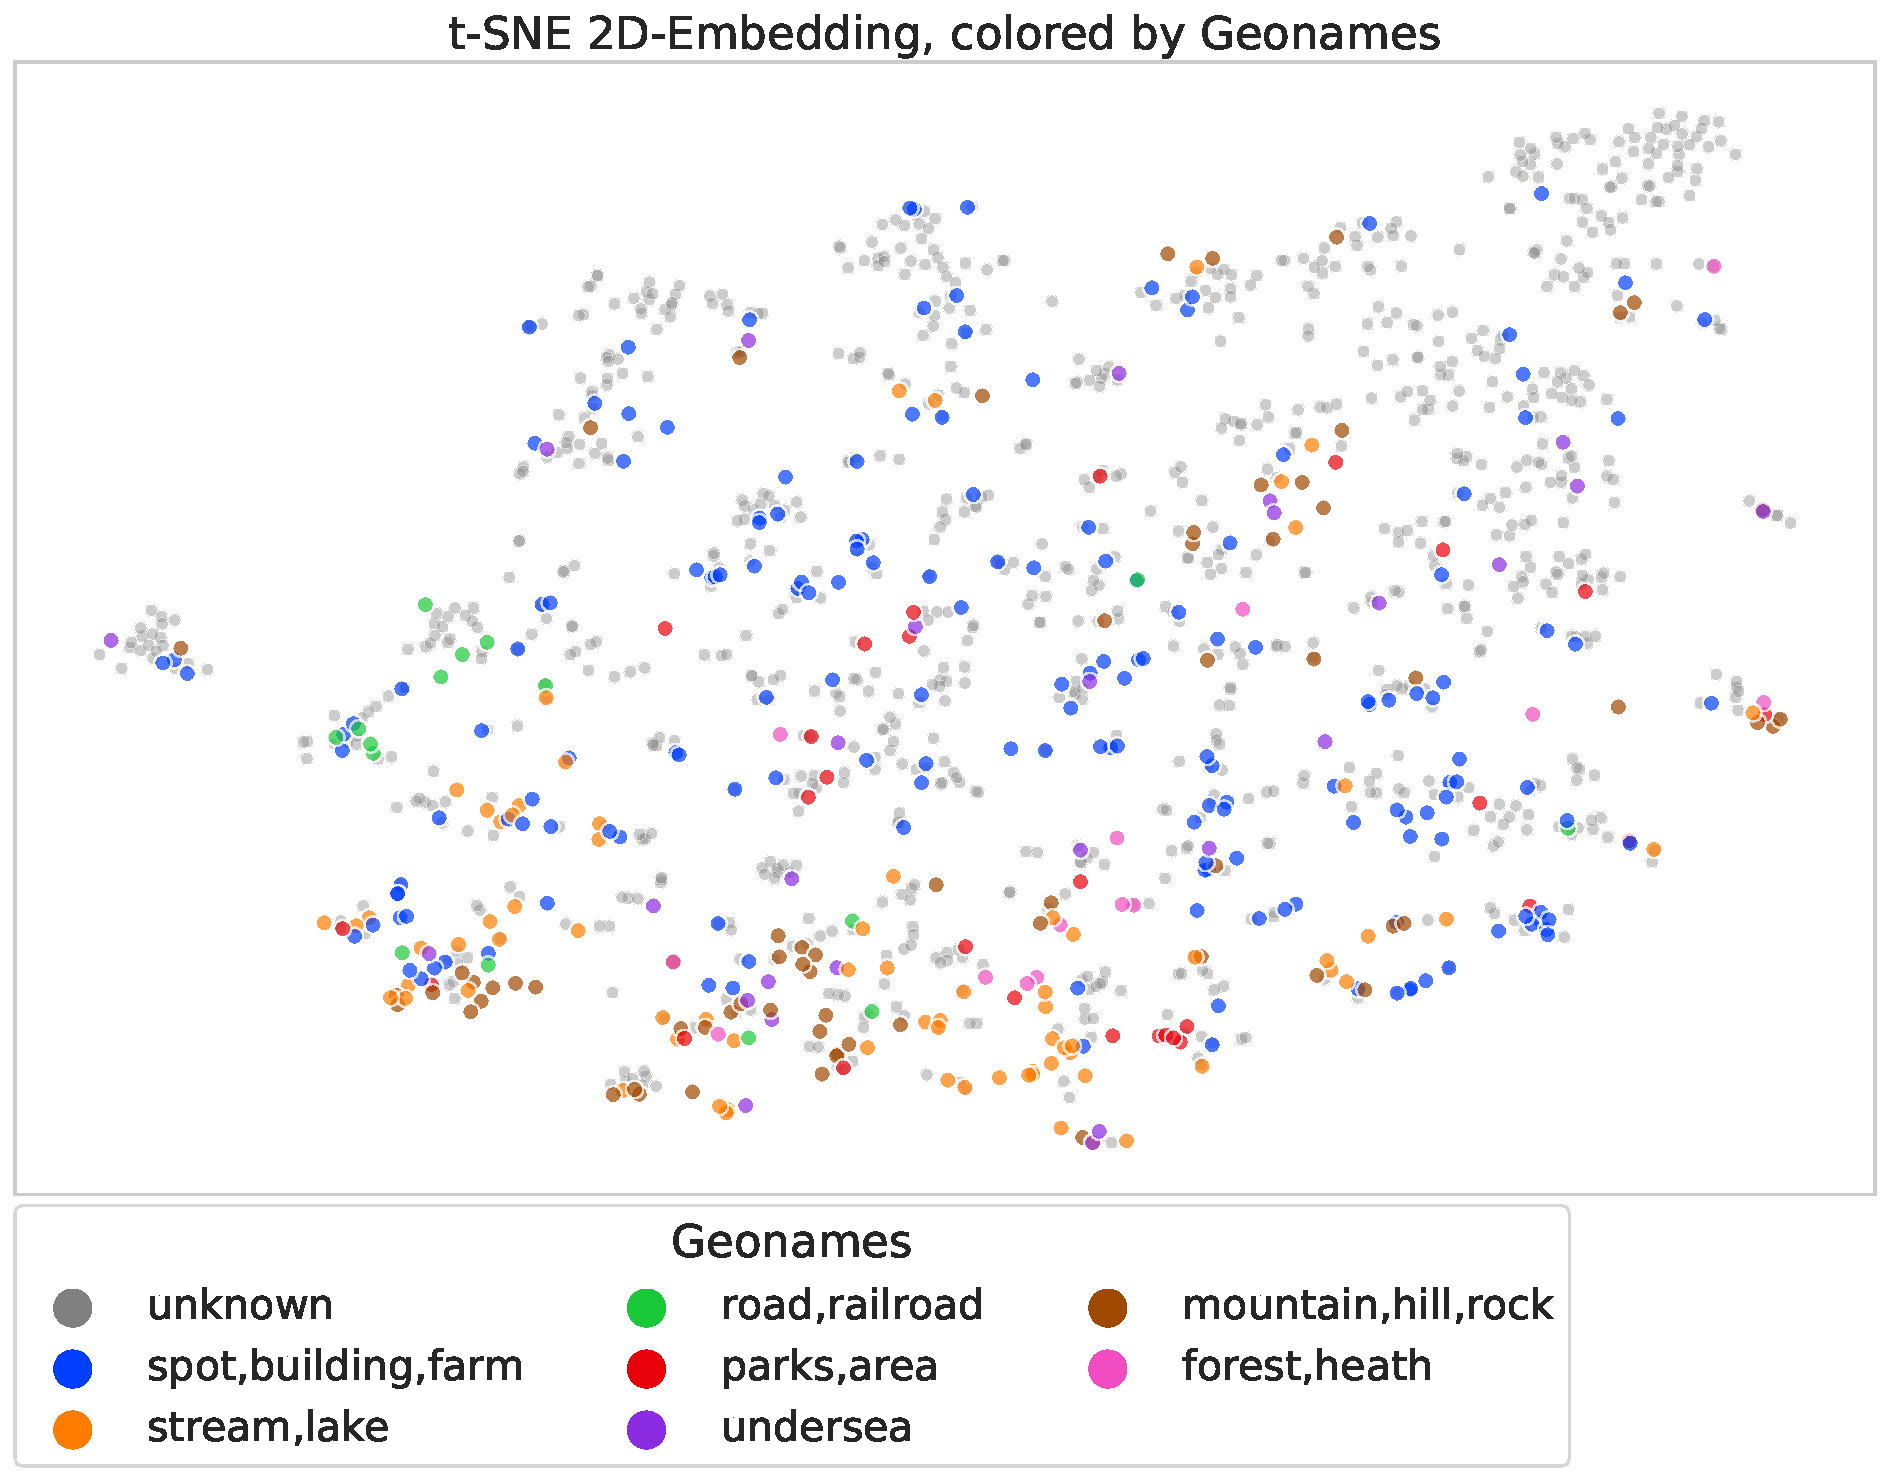
\includegraphics[width=\textwidth]{graphics/figures/scatter_mds_tsne_places_Geonames.pdf}
	  \slcaption{2D Visualization of the Placetypes-Dissimilarity-Matrix \todoparagraph{not mine, but the one of Derrac}, generated with \gls{tsne}. See \url{https://github.com/cstenkamp/derive_conceptualspaces/blob/main/notebooks/text_referenced_plots/desc15_mds_2d3d.ipynb} for the origin of this plot.}
	  \label{fig:scatter_mds_placetypes}
      %TODO: "colored by Geonames"
	\end{center}
\end{figure}


\begin{figure}[h]
	\begin{center}
	  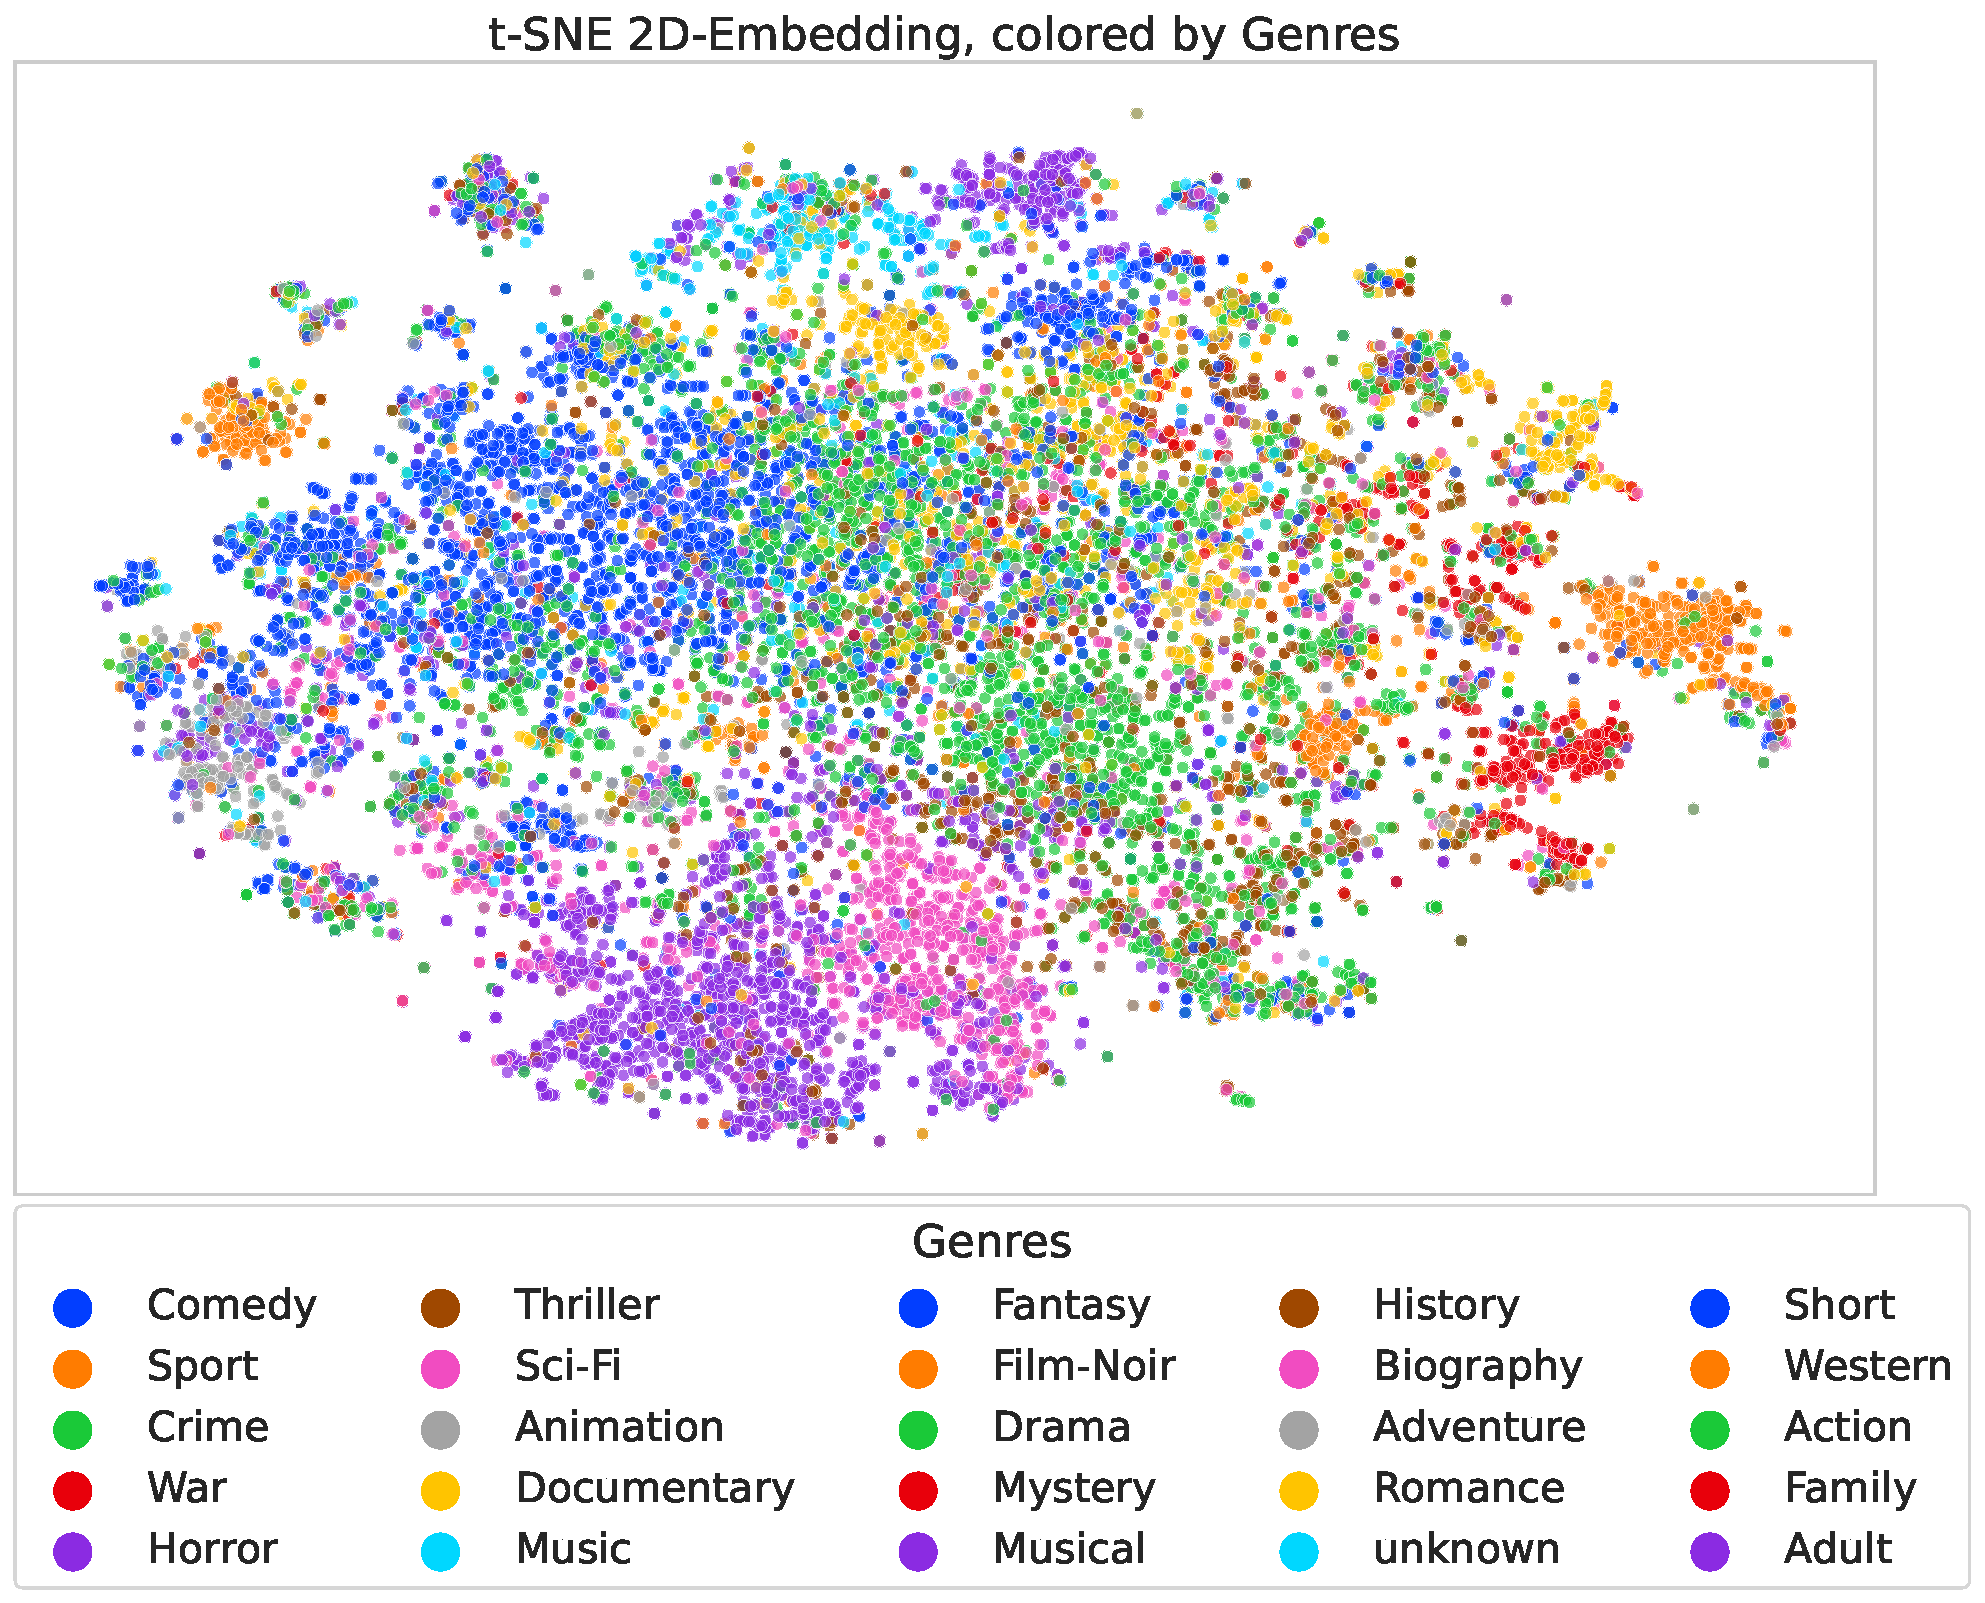
\includegraphics[width=\textwidth]{graphics/figures/scatter_mds_tsne_movies_Genres.pdf}
	  \slcaption{2D Visualization of the Movie-Dissimilarity-Matrix, generated with \gls{tsne}. See \url{https://github.com/cstenkamp/derive_conceptualspaces/blob/main/notebooks/text_referenced_plots/desc15_mds_2d3d.ipynb} for the origin of this plot.}
	  \label{fig:scatter_mds_movies}
      %TODO: "colored by genre"
	\end{center}
\end{figure}


\todoparagraph{Note that at} \url{https://github.com/cstenkamp/derive_conceptualspaces/blob/main/notebooks/text_referenced_plots/desc15_mds_2d3d.ipynb} there are also interactive 3D-Versions of these plots. The one for the SIDDATA-dataset is at \url{https://github.com/cstenkamp/derive_conceptualspaces/blob/main/notebooks/text_referenced_plots/visualize_embeddings.ipynb}, also 2D and interactive 3D. 

\clearpage
\section{Results for Classifiers on placetypes}

\begin{table}[H]
	\centering
	\makebox[\textwidth][c]{
		\resizebox{1.2\textwidth}{!}{%
		\begin{tabular}{rr|ccccc|ccccc|cc|cc}
		&
		&
		\multicolumn{5}{c|}{\textbf{\textcite{Alshaikh2020} (MDS)}} &
		\multicolumn{5}{c|}{\textbf{\textcite{Ager2018}}} &
		\multicolumn{2}{c|}{\textbf{\textcite{Derrac2015}}} &
		\multicolumn{2}{c}{\textbf{This work}} \\
		&
		&
		\textbf{Random} &
		\textbf{AHC} &
		\textbf{Primary} &
		\textbf{Sub} &
		\textbf{Ortho} &
		\textbf{FT MDS} &
		\textbf{MDS} &
		\textbf{FT AWV} &
		\textbf{AWV} &
		\textbf{LDA} &
		\textbf{Best} &
		\textbf{Best BL} &
		\textbf{Best-all} &
		\textbf{Mean-Best} \\ \midrule
		\textbf{Foursquare} &
		\textbf{D1} &
		0.39 &
		0.36 &
		0.36 &
		0.43 &
		\textbf{0.45} &
		0.41 &
		0.38 &
		0.39 &
		0.32 &
		\textbf{0.55} &
		\multicolumn{2}{c|}{-} &
		\textbf{0.50} & 0.45
		\\
		&
		\textbf{D3} &
		0.50 &
		0.46 &
		0.48 &
		0.54 &
		\textbf{0.57} &
		0.44 &
		0.42 &
		0.42 &
		0.37 &
		0.48 &
		\multicolumn{2}{c|}{-} &
		\textbf{0.58} & 0.5
		\\
		&
		\textbf{DN} &
		\multicolumn{5}{c|}{-} &
		0.41 &
		0.42 &
		0.41 &
		0.31 &
		0.47 &
		\textbf{0.53} &
		\textbf{0.53} &
		\textbf{0.57} & 0.55
		\\
		\multicolumn{1}{l}{} &
		\multicolumn{1}{l|}{\textbf{Any}} &
		\multicolumn{5}{c|}{-} &
		\multicolumn{5}{c|}{-} &
		\textbf{0.73} &
		0.72 &
		- & -
		\\
		\textbf{Geonames} &
		\textbf{D1} &
		0.23 &
		0.22 &
		0.24 &
		0.20 &
		0.28 &
		0.32 &
		\textbf{0.32} &
		0.31 &
		0.28 &
		\textbf{0.34} &
		\multicolumn{2}{c|}{-} &
		\textbf{0.51} & 0.48
		\\
		&
		\textbf{D3} &
		0.27 &
		0.29 &
		0.27 &
		0.32 &
		\textbf{0.34} &
		0.31 &
		0.31 &
		0.29 &
		0.28 &
		0.32 &
		\multicolumn{2}{c|}{-} &
		\textbf{0.54} & 0.51
		\\
		&
		\textbf{DN} &
		\multicolumn{5}{c|}{-} &
		0.24 &
		0.21 &
		0.23 &
		0.22 &
		0.27 &
		\textbf{0.37} &
		0.2 &
		\textbf{0.46} & 0.44
		\\
		\multicolumn{1}{l}{} &
		\multicolumn{1}{l|}{\textbf{Any}} &
		\multicolumn{5}{c|}{-} &
		\multicolumn{5}{c|}{-} &
		\textbf{0.41} &
		0.36 &
		- & -
		
		\end{tabular}%
		} % resizebox
	} % makebox
	\caption{F1-Scores of classifiers predicting GeoNames- and Foursquare-labels for baselines, \mainalgos and this work (long)}
	\label{tab:f1_placetypes_long}
\end{table}


\autoref{tab:f1_placetypes_long} is a longer version of \autoref{tab:f1_mainalgos_me_short}, reporting F1-Scores of classifiers predicting GeoNames- and Foursquare-labels for baselines, \mainalgos and this work. 
\textbf{Cls} column encodes the classifier: \textbf{D1/3} are \glspl{dt} of depth 1/3, \textbf{DN} an unbounded \gls{dt}. Condition \textbf{Any} refers to the best of all semantic classifiers developed by \cite{Derrac2015}. \\
First five columns are the exact results reported by \cite{Alshaikh2020}, next five columns those by \cite{Ager2018}, afterwards the best config of \cite{Derrac2015} and the best baseline-condition of \cite{Derrac2015}. The exact conditions of that work are (left to right, top to bottom): C4.5\textsubscript{dir}, C4.5\textsubscript{MDS}, Col, 1-NN (100D), C4.5\textsubscript{dir}, C4.5\textsubscript{MDS}, Analog\textsubscript{C}, 1-NN (50D). Explanations of the respective conditions can be found in their work. \\
All scores are reported with a train-test split of 70\% to 30\%. Note that the reported results of \cite{Ager2018} are unrepresentive when compared to the other datasets: For the placetypes-dataset, \textbf{LDA} performs consistently better than their methods, which is not the case for all other datasets used by them. In the case of \cite{Alshaikh2020}, the results for the placetypes-dataset seem to indicate that the \textbf{Ortho}-condition performs consistently better than the \textbf{Sub}-condition, which was however not the case for any of the other datasets the authors considered. \\
Final columns are the results of this work. Column \textbf{Best-all} encodes a different for each row, specifically the one that yields the best result for the respective classification task, whereas column \textbf{Mean-Best} refers to the single configuration that achieved the best results on average.

\section{F1-scores per Faculty}


\begin{table}[H]
	\resizebox{\textwidth}{!}{%
		\begin{tabular}{rcccc}
		\toprule
		\textbf{Depth} & \textbf{1} & \textbf{2} & \textbf{3} & \textbf{unbound} \\
		\midrule
		\textbf{Sozialwissenschaften} & 0.386 ± 0.029 & 0.414 ± 0.031 & 0.403 ± 0.024 & 0.580 ± 0.034 \\
		\textbf{Kultur-/Geowissenschaften} & 0.454 ± 0.023 & 0.514 ± 0.034 & 0.591 ± 0.026 & 0.685 ± 0.020 \\
		\textbf{Erziehungs-/Kulturwissenschaften} & 0.600 ± 0.019 & 0.701 ± 0.015 & 0.713 ± 0.019 & 0.765 ± 0.015 \\
		\textbf{Physik} & 0.096 ± 0.019 & 0.117 ± 0.012 & 0.145 ± 0.023 & 0.552 ± 0.072 \\
		\textbf{Biologie/Chemie} & 0.133 ± 0.019 & 0.178 ± 0.043 & 0.247 ± 0.063 & 0.611 ± 0.084 \\
		\textbf{Mathematik/Informatik} & 0.215 ± 0.032 & 0.211 ± 0.046 & 0.260 ± 0.057 & 0.542 ± 0.070 \\
		\textbf{Sprach-/Literaturwissenschaften} & 0.652 ± 0.020 & 0.685 ± 0.014 & 0.733 ± 0.014 & 0.790 ± 0.017 \\
		\textbf{Humanwissenschaften} & 0.177 ± 0.028 & 0.245 ± 0.061 & 0.276 ± 0.078 & 0.484 ± 0.043 \\
		\textbf{Wirtschaftswissenschaften} & 0.198 ± 0.022 & 0.219 ± 0.059 & 0.236 ± 0.040 & 0.596 ± 0.084 \\
		\textbf{Rechtswissenschaften} & 0.617 ± 0.108 & 0.456 ± 0.037 & 0.641 ± 0.050 & 0.841 ± 0.032 \\
		\textbf{Mean (weighted)} & 0.505 ± 0.026 & 0.553 ± 0.026 & 0.597 ± 0.026 & 0.710 ± 0.026 \\
		\textbf{Mean (unweighted)} & 0.353 ± 0.032 & 0.374 ± 0.035 & 0.424 ± 0.039 & 0.645 ± 0.047 \\
		\bottomrule
		\end{tabular}
	}
	\slcaption{Robust F1-scores per Faculty of a well-performing configuration. The reported results are mean and standard deviation from the result of ten runs with 5-fold crossvalidation each.}
	\label{tab:robustresults_perfb_f1}
\end{table}


\section{Sample Classification}


\begin{figure}[h]
	\begin{center}
	  \makebox[\textwidth][c]{
		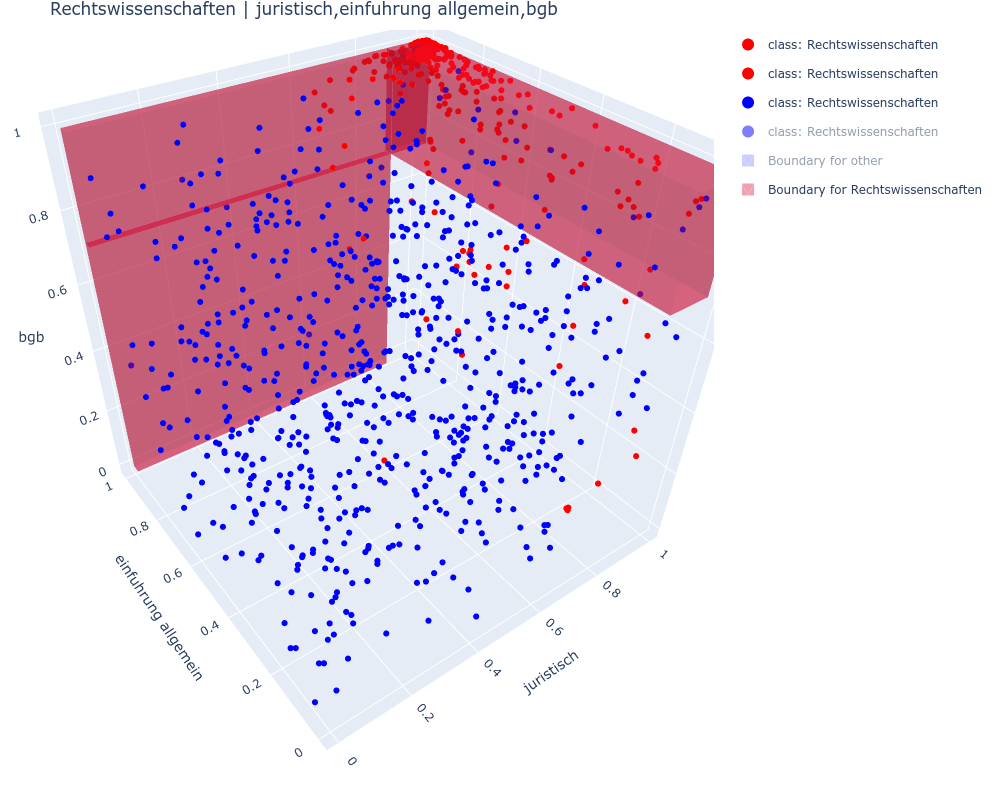
\includegraphics[width=1.1\textwidth]{graphics/dataset_new/boxes_rechtswis.png}
		\slcaption{A classification with a Level-2-Decisiontree. Visualize in 3D: \url{https://github.com/cstenkamp/derive_conceptualspaces/blob/main/notebooks/text_referenced_plots/display_top3_SIDDATA.ipynb} }
		\label{fig:boxes_rechtswis}
		% möchte sagen: How does a decision look graphically, and how does it compare to the original 3D?
		% TODO: add accuracy 
	  }
	\end{center}
\end{figure}

	\chapter{Algorithm as Pseudo-Code}
\label{ap:algorithm_pseudo}

% \todoparagraph{make this compliant with my minimal implementation of the steps}

\input{pandoc_generated_latex/6_4_algoritm_pseudocode}


	\cleardoublepage
\pagestyle{plain}
\bookmarksetup{startatroot} 

\printbibliography[heading=bibintoc]

\end{document}